
\documentclass[10pt]{article} % For LaTeX2e
\usepackage{iclr2025_conference}
\usepackage{times}

\iclrfinalcopy

% Optional math commands from https://github.com/goodfeli/dlbook_notation.
%%%%% NEW MATH DEFINITIONS %%%%%

\usepackage{amsmath,amsfonts,bm}

% Mark sections of captions for referring to divisions of figures
\newcommand{\figleft}{{\em (Left)}}
\newcommand{\figcenter}{{\em (Center)}}
\newcommand{\figright}{{\em (Right)}}
\newcommand{\figtop}{{\em (Top)}}
\newcommand{\figbottom}{{\em (Bottom)}}
\newcommand{\captiona}{{\em (a)}}
\newcommand{\captionb}{{\em (b)}}
\newcommand{\captionc}{{\em (c)}}
\newcommand{\captiond}{{\em (d)}}

% Highlight a newly defined term
\newcommand{\newterm}[1]{{\bf #1}}


% Figure reference, lower-case.
\def\figref#1{figure~\ref{#1}}
% Figure reference, capital. For start of sentence
\def\Figref#1{Figure~\ref{#1}}
\def\twofigref#1#2{figures \ref{#1} and \ref{#2}}
\def\quadfigref#1#2#3#4{figures \ref{#1}, \ref{#2}, \ref{#3} and \ref{#4}}
% Section reference, lower-case.
\def\secref#1{section~\ref{#1}}
% Section reference, capital.
\def\Secref#1{Section~\ref{#1}}
% Reference to two sections.
\def\twosecrefs#1#2{sections \ref{#1} and \ref{#2}}
% Reference to three sections.
\def\secrefs#1#2#3{sections \ref{#1}, \ref{#2} and \ref{#3}}
% Reference to an equation, lower-case.
\def\eqref#1{equation~\ref{#1}}
% Reference to an equation, upper case
\def\Eqref#1{Equation~\ref{#1}}
% A raw reference to an equation---avoid using if possible
\def\plaineqref#1{\ref{#1}}
% Reference to a chapter, lower-case.
\def\chapref#1{chapter~\ref{#1}}
% Reference to an equation, upper case.
\def\Chapref#1{Chapter~\ref{#1}}
% Reference to a range of chapters
\def\rangechapref#1#2{chapters\ref{#1}--\ref{#2}}
% Reference to an algorithm, lower-case.
\def\algref#1{algorithm~\ref{#1}}
% Reference to an algorithm, upper case.
\def\Algref#1{Algorithm~\ref{#1}}
\def\twoalgref#1#2{algorithms \ref{#1} and \ref{#2}}
\def\Twoalgref#1#2{Algorithms \ref{#1} and \ref{#2}}
% Reference to a part, lower case
\def\partref#1{part~\ref{#1}}
% Reference to a part, upper case
\def\Partref#1{Part~\ref{#1}}
\def\twopartref#1#2{parts \ref{#1} and \ref{#2}}

\def\ceil#1{\lceil #1 \rceil}
\def\floor#1{\lfloor #1 \rfloor}
\def\1{\bm{1}}
\newcommand{\train}{\mathcal{D}}
\newcommand{\valid}{\mathcal{D_{\mathrm{valid}}}}
\newcommand{\test}{\mathcal{D_{\mathrm{test}}}}

\def\eps{{\epsilon}}


% Random variables
\def\reta{{\textnormal{$\eta$}}}
\def\ra{{\textnormal{a}}}
\def\rb{{\textnormal{b}}}
\def\rc{{\textnormal{c}}}
\def\rd{{\textnormal{d}}}
\def\re{{\textnormal{e}}}
\def\rf{{\textnormal{f}}}
\def\rg{{\textnormal{g}}}
\def\rh{{\textnormal{h}}}
\def\ri{{\textnormal{i}}}
\def\rj{{\textnormal{j}}}
\def\rk{{\textnormal{k}}}
\def\rl{{\textnormal{l}}}
% rm is already a command, just don't name any random variables m
\def\rn{{\textnormal{n}}}
\def\ro{{\textnormal{o}}}
\def\rp{{\textnormal{p}}}
\def\rq{{\textnormal{q}}}
\def\rr{{\textnormal{r}}}
\def\rs{{\textnormal{s}}}
\def\rt{{\textnormal{t}}}
\def\ru{{\textnormal{u}}}
\def\rv{{\textnormal{v}}}
\def\rw{{\textnormal{w}}}
\def\rx{{\textnormal{x}}}
\def\ry{{\textnormal{y}}}
\def\rz{{\textnormal{z}}}

% Random vectors
\def\rvepsilon{{\mathbf{\epsilon}}}
\def\rvtheta{{\mathbf{\theta}}}
\def\rva{{\mathbf{a}}}
\def\rvb{{\mathbf{b}}}
\def\rvc{{\mathbf{c}}}
\def\rvd{{\mathbf{d}}}
\def\rve{{\mathbf{e}}}
\def\rvf{{\mathbf{f}}}
\def\rvg{{\mathbf{g}}}
\def\rvh{{\mathbf{h}}}
\def\rvu{{\mathbf{i}}}
\def\rvj{{\mathbf{j}}}
\def\rvk{{\mathbf{k}}}
\def\rvl{{\mathbf{l}}}
\def\rvm{{\mathbf{m}}}
\def\rvn{{\mathbf{n}}}
\def\rvo{{\mathbf{o}}}
\def\rvp{{\mathbf{p}}}
\def\rvq{{\mathbf{q}}}
\def\rvr{{\mathbf{r}}}
\def\rvs{{\mathbf{s}}}
\def\rvt{{\mathbf{t}}}
\def\rvu{{\mathbf{u}}}
\def\rvv{{\mathbf{v}}}
\def\rvw{{\mathbf{w}}}
\def\rvx{{\mathbf{x}}}
\def\rvy{{\mathbf{y}}}
\def\rvz{{\mathbf{z}}}

% Elements of random vectors
\def\erva{{\textnormal{a}}}
\def\ervb{{\textnormal{b}}}
\def\ervc{{\textnormal{c}}}
\def\ervd{{\textnormal{d}}}
\def\erve{{\textnormal{e}}}
\def\ervf{{\textnormal{f}}}
\def\ervg{{\textnormal{g}}}
\def\ervh{{\textnormal{h}}}
\def\ervi{{\textnormal{i}}}
\def\ervj{{\textnormal{j}}}
\def\ervk{{\textnormal{k}}}
\def\ervl{{\textnormal{l}}}
\def\ervm{{\textnormal{m}}}
\def\ervn{{\textnormal{n}}}
\def\ervo{{\textnormal{o}}}
\def\ervp{{\textnormal{p}}}
\def\ervq{{\textnormal{q}}}
\def\ervr{{\textnormal{r}}}
\def\ervs{{\textnormal{s}}}
\def\ervt{{\textnormal{t}}}
\def\ervu{{\textnormal{u}}}
\def\ervv{{\textnormal{v}}}
\def\ervw{{\textnormal{w}}}
\def\ervx{{\textnormal{x}}}
\def\ervy{{\textnormal{y}}}
\def\ervz{{\textnormal{z}}}

% Random matrices
\def\rmA{{\mathbf{A}}}
\def\rmB{{\mathbf{B}}}
\def\rmC{{\mathbf{C}}}
\def\rmD{{\mathbf{D}}}
\def\rmE{{\mathbf{E}}}
\def\rmF{{\mathbf{F}}}
\def\rmG{{\mathbf{G}}}
\def\rmH{{\mathbf{H}}}
\def\rmI{{\mathbf{I}}}
\def\rmJ{{\mathbf{J}}}
\def\rmK{{\mathbf{K}}}
\def\rmL{{\mathbf{L}}}
\def\rmM{{\mathbf{M}}}
\def\rmN{{\mathbf{N}}}
\def\rmO{{\mathbf{O}}}
\def\rmP{{\mathbf{P}}}
\def\rmQ{{\mathbf{Q}}}
\def\rmR{{\mathbf{R}}}
\def\rmS{{\mathbf{S}}}
\def\rmT{{\mathbf{T}}}
\def\rmU{{\mathbf{U}}}
\def\rmV{{\mathbf{V}}}
\def\rmW{{\mathbf{W}}}
\def\rmX{{\mathbf{X}}}
\def\rmY{{\mathbf{Y}}}
\def\rmZ{{\mathbf{Z}}}

% Elements of random matrices
\def\ermA{{\textnormal{A}}}
\def\ermB{{\textnormal{B}}}
\def\ermC{{\textnormal{C}}}
\def\ermD{{\textnormal{D}}}
\def\ermE{{\textnormal{E}}}
\def\ermF{{\textnormal{F}}}
\def\ermG{{\textnormal{G}}}
\def\ermH{{\textnormal{H}}}
\def\ermI{{\textnormal{I}}}
\def\ermJ{{\textnormal{J}}}
\def\ermK{{\textnormal{K}}}
\def\ermL{{\textnormal{L}}}
\def\ermM{{\textnormal{M}}}
\def\ermN{{\textnormal{N}}}
\def\ermO{{\textnormal{O}}}
\def\ermP{{\textnormal{P}}}
\def\ermQ{{\textnormal{Q}}}
\def\ermR{{\textnormal{R}}}
\def\ermS{{\textnormal{S}}}
\def\ermT{{\textnormal{T}}}
\def\ermU{{\textnormal{U}}}
\def\ermV{{\textnormal{V}}}
\def\ermW{{\textnormal{W}}}
\def\ermX{{\textnormal{X}}}
\def\ermY{{\textnormal{Y}}}
\def\ermZ{{\textnormal{Z}}}

% Vectors
\def\vzero{{\bm{0}}}
\def\vone{{\bm{1}}}
\def\vmu{{\bm{\mu}}}
\def\vtheta{{\bm{\theta}}}
\def\va{{\bm{a}}}
\def\vb{{\bm{b}}}
\def\vc{{\bm{c}}}
\def\vd{{\bm{d}}}
\def\ve{{\bm{e}}}
\def\vf{{\bm{f}}}
\def\vg{{\bm{g}}}
\def\vh{{\bm{h}}}
\def\vi{{\bm{i}}}
\def\vj{{\bm{j}}}
\def\vk{{\bm{k}}}
\def\vl{{\bm{l}}}
\def\vm{{\bm{m}}}
\def\vn{{\bm{n}}}
\def\vo{{\bm{o}}}
\def\vp{{\bm{p}}}
\def\vq{{\bm{q}}}
\def\vr{{\bm{r}}}
\def\vs{{\bm{s}}}
\def\vt{{\bm{t}}}
\def\vu{{\bm{u}}}
\def\vv{{\bm{v}}}
\def\vw{{\bm{w}}}
\def\vx{{\bm{x}}}
\def\vy{{\bm{y}}}
\def\vz{{\bm{z}}}

% Elements of vectors
\def\evalpha{{\alpha}}
\def\evbeta{{\beta}}
\def\evepsilon{{\epsilon}}
\def\evlambda{{\lambda}}
\def\evomega{{\omega}}
\def\evmu{{\mu}}
\def\evpsi{{\psi}}
\def\evsigma{{\sigma}}
\def\evtheta{{\theta}}
\def\eva{{a}}
\def\evb{{b}}
\def\evc{{c}}
\def\evd{{d}}
\def\eve{{e}}
\def\evf{{f}}
\def\evg{{g}}
\def\evh{{h}}
\def\evi{{i}}
\def\evj{{j}}
\def\evk{{k}}
\def\evl{{l}}
\def\evm{{m}}
\def\evn{{n}}
\def\evo{{o}}
\def\evp{{p}}
\def\evq{{q}}
\def\evr{{r}}
\def\evs{{s}}
\def\evt{{t}}
\def\evu{{u}}
\def\evv{{v}}
\def\evw{{w}}
\def\evx{{x}}
\def\evy{{y}}
\def\evz{{z}}

% Matrix
\def\mA{{\bm{A}}}
\def\mB{{\bm{B}}}
\def\mC{{\bm{C}}}
\def\mD{{\bm{D}}}
\def\mE{{\bm{E}}}
\def\mF{{\bm{F}}}
\def\mG{{\bm{G}}}
\def\mH{{\bm{H}}}
\def\mI{{\bm{I}}}
\def\mJ{{\bm{J}}}
\def\mK{{\bm{K}}}
\def\mL{{\bm{L}}}
\def\mM{{\bm{M}}}
\def\mN{{\bm{N}}}
\def\mO{{\bm{O}}}
\def\mP{{\bm{P}}}
\def\mQ{{\bm{Q}}}
\def\mR{{\bm{R}}}
\def\mS{{\bm{S}}}
\def\mT{{\bm{T}}}
\def\mU{{\bm{U}}}
\def\mV{{\bm{V}}}
\def\mW{{\bm{W}}}
\def\mX{{\bm{X}}}
\def\mY{{\bm{Y}}}
\def\mZ{{\bm{Z}}}
\def\mBeta{{\bm{\beta}}}
\def\mPhi{{\bm{\Phi}}}
\def\mLambda{{\bm{\Lambda}}}
\def\mSigma{{\bm{\Sigma}}}

% Tensor
\DeclareMathAlphabet{\mathsfit}{\encodingdefault}{\sfdefault}{m}{sl}
\SetMathAlphabet{\mathsfit}{bold}{\encodingdefault}{\sfdefault}{bx}{n}
\newcommand{\tens}[1]{\bm{\mathsfit{#1}}}
\def\tA{{\tens{A}}}
\def\tB{{\tens{B}}}
\def\tC{{\tens{C}}}
\def\tD{{\tens{D}}}
\def\tE{{\tens{E}}}
\def\tF{{\tens{F}}}
\def\tG{{\tens{G}}}
\def\tH{{\tens{H}}}
\def\tI{{\tens{I}}}
\def\tJ{{\tens{J}}}
\def\tK{{\tens{K}}}
\def\tL{{\tens{L}}}
\def\tM{{\tens{M}}}
\def\tN{{\tens{N}}}
\def\tO{{\tens{O}}}
\def\tP{{\tens{P}}}
\def\tQ{{\tens{Q}}}
\def\tR{{\tens{R}}}
\def\tS{{\tens{S}}}
\def\tT{{\tens{T}}}
\def\tU{{\tens{U}}}
\def\tV{{\tens{V}}}
\def\tW{{\tens{W}}}
\def\tX{{\tens{X}}}
\def\tY{{\tens{Y}}}
\def\tZ{{\tens{Z}}}


% Graph
\def\gA{{\mathcal{A}}}
\def\gB{{\mathcal{B}}}
\def\gC{{\mathcal{C}}}
\def\gD{{\mathcal{D}}}
\def\gE{{\mathcal{E}}}
\def\gF{{\mathcal{F}}}
\def\gG{{\mathcal{G}}}
\def\gH{{\mathcal{H}}}
\def\gI{{\mathcal{I}}}
\def\gJ{{\mathcal{J}}}
\def\gK{{\mathcal{K}}}
\def\gL{{\mathcal{L}}}
\def\gM{{\mathcal{M}}}
\def\gN{{\mathcal{N}}}
\def\gO{{\mathcal{O}}}
\def\gP{{\mathcal{P}}}
\def\gQ{{\mathcal{Q}}}
\def\gR{{\mathcal{R}}}
\def\gS{{\mathcal{S}}}
\def\gT{{\mathcal{T}}}
\def\gU{{\mathcal{U}}}
\def\gV{{\mathcal{V}}}
\def\gW{{\mathcal{W}}}
\def\gX{{\mathcal{X}}}
\def\gY{{\mathcal{Y}}}
\def\gZ{{\mathcal{Z}}}

% Sets
\def\sA{{\mathbb{A}}}
\def\sB{{\mathbb{B}}}
\def\sC{{\mathbb{C}}}
\def\sD{{\mathbb{D}}}
% Don't use a set called E, because this would be the same as our symbol
% for expectation.
\def\sF{{\mathbb{F}}}
\def\sG{{\mathbb{G}}}
\def\sH{{\mathbb{H}}}
\def\sI{{\mathbb{I}}}
\def\sJ{{\mathbb{J}}}
\def\sK{{\mathbb{K}}}
\def\sL{{\mathbb{L}}}
\def\sM{{\mathbb{M}}}
\def\sN{{\mathbb{N}}}
\def\sO{{\mathbb{O}}}
\def\sP{{\mathbb{P}}}
\def\sQ{{\mathbb{Q}}}
\def\sR{{\mathbb{R}}}
\def\sS{{\mathbb{S}}}
\def\sT{{\mathbb{T}}}
\def\sU{{\mathbb{U}}}
\def\sV{{\mathbb{V}}}
\def\sW{{\mathbb{W}}}
\def\sX{{\mathbb{X}}}
\def\sY{{\mathbb{Y}}}
\def\sZ{{\mathbb{Z}}}

% Entries of a matrix
\def\emLambda{{\Lambda}}
\def\emA{{A}}
\def\emB{{B}}
\def\emC{{C}}
\def\emD{{D}}
\def\emE{{E}}
\def\emF{{F}}
\def\emG{{G}}
\def\emH{{H}}
\def\emI{{I}}
\def\emJ{{J}}
\def\emK{{K}}
\def\emL{{L}}
\def\emM{{M}}
\def\emN{{N}}
\def\emO{{O}}
\def\emP{{P}}
\def\emQ{{Q}}
\def\emR{{R}}
\def\emS{{S}}
\def\emT{{T}}
\def\emU{{U}}
\def\emV{{V}}
\def\emW{{W}}
\def\emX{{X}}
\def\emY{{Y}}
\def\emZ{{Z}}
\def\emSigma{{\Sigma}}

% entries of a tensor
% Same font as tensor, without \bm wrapper
\newcommand{\etens}[1]{\mathsfit{#1}}
\def\etLambda{{\etens{\Lambda}}}
\def\etA{{\etens{A}}}
\def\etB{{\etens{B}}}
\def\etC{{\etens{C}}}
\def\etD{{\etens{D}}}
\def\etE{{\etens{E}}}
\def\etF{{\etens{F}}}
\def\etG{{\etens{G}}}
\def\etH{{\etens{H}}}
\def\etI{{\etens{I}}}
\def\etJ{{\etens{J}}}
\def\etK{{\etens{K}}}
\def\etL{{\etens{L}}}
\def\etM{{\etens{M}}}
\def\etN{{\etens{N}}}
\def\etO{{\etens{O}}}
\def\etP{{\etens{P}}}
\def\etQ{{\etens{Q}}}
\def\etR{{\etens{R}}}
\def\etS{{\etens{S}}}
\def\etT{{\etens{T}}}
\def\etU{{\etens{U}}}
\def\etV{{\etens{V}}}
\def\etW{{\etens{W}}}
\def\etX{{\etens{X}}}
\def\etY{{\etens{Y}}}
\def\etZ{{\etens{Z}}}

% The true underlying data generating distribution
\newcommand{\pdata}{p_{\rm{data}}}
% The empirical distribution defined by the training set
\newcommand{\ptrain}{\hat{p}_{\rm{data}}}
\newcommand{\Ptrain}{\hat{P}_{\rm{data}}}
% The model distribution
\newcommand{\pmodel}{p_{\rm{model}}}
\newcommand{\Pmodel}{P_{\rm{model}}}
\newcommand{\ptildemodel}{\tilde{p}_{\rm{model}}}
% Stochastic autoencoder distributions
\newcommand{\pencode}{p_{\rm{encoder}}}
\newcommand{\pdecode}{p_{\rm{decoder}}}
\newcommand{\precons}{p_{\rm{reconstruct}}}

\newcommand{\laplace}{\mathrm{Laplace}} % Laplace distribution

\newcommand{\E}{\mathbb{E}}
\newcommand{\Ls}{\mathcal{L}}
\newcommand{\R}{\mathbb{R}}
\newcommand{\emp}{\tilde{p}}
\newcommand{\lr}{\alpha}
\newcommand{\reg}{\lambda}
\newcommand{\rect}{\mathrm{rectifier}}
\newcommand{\softmax}{\mathrm{softmax}}
\newcommand{\sigmoid}{\sigma}
\newcommand{\softplus}{\zeta}
\newcommand{\KL}{D_{\mathrm{KL}}}
\newcommand{\Var}{\mathrm{Var}}
\newcommand{\standarderror}{\mathrm{SE}}
\newcommand{\Cov}{\mathrm{Cov}}
% Wolfram Mathworld says $L^2$ is for function spaces and $\ell^2$ is for vectors
% But then they seem to use $L^2$ for vectors throughout the site, and so does
% wikipedia.
\newcommand{\normlzero}{L^0}
\newcommand{\normlone}{L^1}
\newcommand{\normltwo}{L^2}
\newcommand{\normlp}{L^p}
\newcommand{\normmax}{L^\infty}

\newcommand{\parents}{Pa} % See usage in notation.tex. Chosen to match Daphne's book.

\DeclareMathOperator*{\argmax}{arg\,max}
\DeclareMathOperator*{\argmin}{arg\,min}

\DeclareMathOperator{\sign}{sign}
\DeclareMathOperator{\Tr}{Tr}
\let\ab\allowbreak

% Custom shit
\newcommand{\bcal}[1]{\bm{\mathcal{#1}}}


\newcommand{\deq}{\mathrel{\mathop:}=} % aligned define equals
\newcommand{\deqrev}{=\mathrel{\mathop:}} % aligned define equals
\newcommand{\ft}{\sigma_\textsc{t}}
\newcommand{\fs}{\sigma}
\newcommand{\bfx}{\mathbf{x}}
\newcommand{\bfy}{\mathbf{y}}
\newcommand{\bft}{\mathbf{\theta}}
\newcommand{\bfe}{\boldsymbol{\varepsilon}}
\DeclareMathOperator{\NN}{N}
\DeclareMathOperator{\diag}{diag}
\newcommand{\bias}{B}
\newcommand{\Etrain}{E_\text{train}}
\newcommand{\Etest}{E_\text{test}}
\DeclareMathOperator{\tr}{tr}
\DeclareMathOperator{\erf}{erf}
\DeclareMathOperator{\Erf}{Erf}
\DeclareMathOperator{\relu}{ReLU}




% shortcut for inline equations and alignments
\newcommand{\eq}[1]{\begin{equation}#1\end{equation}}
\newcommand{\eqs}[1]{\begin{equation*}#1\end{equation*}}
\newcommand{\al}[1]{\begin{align}#1\end{align}}
\newcommand{\als}[1]{\begin{align*}#1\end{align*}}
\newcommand{\ca}[1]{\begin{cases}#1\end{cases}}

% ( round parentheses )
\newcommand{\p}[1]{({#1})}
\newcommand{\pb}[1]{\bigl({#1}\bigr)}
\newcommand{\pB}[1]{\Bigl({#1}\Bigr)}
\newcommand{\pbb}[1]{\biggl({#1}\biggr)}
\newcommand{\pBB}[1]{\Biggl({#1}\Biggr)}
\newcommand{\pa}[1]{\left({#1}\right)}

% [ square brackets ]
\newcommand{\q}[1]{[{#1}]}
\newcommand{\qb}[1]{\bigl[{#1}\bigr]}
\newcommand{\qB}[1]{\Bigl[{#1}\Bigr]}
\newcommand{\qbb}[1]{\biggl[{#1}\biggr]}
\newcommand{\qBB}[1]{\Biggl[{#1}\Biggr]}
\newcommand{\qa}[1]{\left[{#1}\right]}

% { curly braces }
\newcommand{\h}[1]{\{{#1}\}}
\newcommand{\hb}[1]{\bigl\{{#1}\bigr\}}
\newcommand{\hB}[1]{\Bigl\{{#1}\Bigr\}}
\newcommand{\hbb}[1]{\biggl\{{#1}\biggr\}}
\newcommand{\hBB}[1]{\Biggl\{{#1}\Biggr\}}
\newcommand{\ha}[1]{\left\{{#1}\right\}}

% | absolute value |
\newcommand{\abs}[1]{\lvert #1 \rvert}
\newcommand{\absb}[1]{\bigl\lvert #1 \bigr\rvert}
\newcommand{\absB}[1]{\Bigl\lvert #1 \Bigr\rvert}
\newcommand{\absbb}[1]{\biggl\lvert #1 \biggr\rvert}
\newcommand{\absBB}[1]{\Biggl\lvert #1 \Biggr\rvert}
\newcommand{\absa}[1]{\left\lvert #1 \right\rvert}

% || norm ||
\newcommand{\norm}[1]{\lVert #1 \rVert}
\newcommand{\normb}[1]{\bigl\lVert #1 \bigr\rVert}
\newcommand{\normB}[1]{\Bigl\lVert #1 \Bigr\rVert}
\newcommand{\normbb}[1]{\biggl\lVert #1 \biggr\rVert}
\newcommand{\normBB}[1]{\Biggl\lVert #1 \Biggr\rVert}
\newcommand{\norma}[1]{\left\lVert #1 \right\rVert}

% End Macros

\newcommand{\bfi}{\mathbf{i}}
\newcommand{\bfj}{\mathbf{j}}
\newcommand{\bfee}{\mathbf{e}}
\newcommand{\bfX}{\mathbf{X}}

\renewcommand{\cal}{\mathcal} % calligraphic
\newcommand{\e}{{\varepsilon}}
\renewcommand{\a}{\alpha}
\newcommand{\be}{\beta}

\newcommand{\V}{\mathbb{V}}

\newcommand{\x}{\times}
\newcommand{\cD}{\mathcal{D}}
\newcommand{\cX}{\mathcal{X}}
\newcommand{\cY}{\mathcal{Y}}
\newcommand{\cL}{\mathcal{L}}
\newcommand{\cA}{\mathcal{A}}
\newcommand{\cT}{\mathcal{T}}

\usepackage{titlesec}
% PACKAGE INCLUSION
\usepackage{amsbsy,amssymb,amsmath,amsfonts,amsthm} % Math and related rendering
\allowdisplaybreaks
\usepackage{tikz-cd,tikz-3dplot,circuitikz} % For graphical drawing
%\usepackage{natbib} % For citation, using numbering style. 
\usepackage{graphicx}
\usepackage{geometry} % configure the geometry page
\usepackage{bbm} % Better bold (for example, \mathbb{1} does not work for font not alphabetical)
\usepackage{bm} % Bold symbol 
\usepackage{tikz} % for normal graphing
\usepackage{enumitem} % for customizing options for lists, enumerations, and descriptions
\usepackage{fancyhdr} % configuring header
\usepackage{parskip} % For paragraph spacing
\usepackage{caption} % captioning options
\usepackage{mathtools} % using this to fix \multlined environment altogether
\usepackage{parnotes}% take this one for marginnote substitute (or the reverse because this one looks so much better)
\usepackage{tabularx} % better tabular
\usepackage{braket} % For bra-ket notation
%\usepackage{fontspec} % does fontspec works for memoir? 
\usepackage{float} % more float control
\usepackage[dvipsnames,svgnames,x11names]{xcolor} % color schema, definitely should have included this
\usetikzlibrary{matrix}
\usepackage{thmtools} % hooks and stuff for listoftheorem
%\DisemulatePackage{showidx} %(2)
%\usepackage{makeidx} % I HATE THIS
%\usepackage{showidx} % I HATE THIS
%\usepackage{subfigure}
\usepackage{caption} % uh, caption
\usepackage{nicematrix} % for drawing matrix
\usepackage{subcaption} % This and the two right above it is required for multi-figure display, so yeah.
%\setcounter{tocdepth}{2}
\usepackage{stmaryrd} % double brackets for integer intervals]
\usepackage{algorithm2e}
\usepackage{algorithmicx}
\usepackage{array}
\usepackage{booktabs}
\newcolumntype{P}[1]{>{\raggedright\arraybackslash}p{#1}}
%-------------------------------%
% CONFIGURING NATBIB
\usepackage{natbib} 
%-------------------------------%
% NEXT IS INDEX CONFIG
%%%%%%%%%%%%%%%%%%%%%%%%%%%
\makeatletter
\renewcommand{\index}[1]{%
  \oldindex{#1}%
  \if@reversemargin
    \marginpar{\raggedleft\small#1}%
  \else
    \marginpar{\raggedright\small#1}%
  \fi
}
\makeatother

%----------------------------------------------------------------------------------% 
% SMALL SETTING
\usepackage{pgfplots} % for something else
\usetikzlibrary{patterns}       % For custom patterns
\usetikzlibrary{shadings}       % For gradient fills
\usetikzlibrary{shapes.geometric} % For geometric shapes
\usetikzlibrary{calc}           % For coordinate calculations
\usetikzlibrary{positioning}    % For node positioning
\usetikzlibrary{decorations.pathreplacing} % For path decorations
\usetikzlibrary{fit} % For fitting shapes around nodes
\newcommand{\calx}[1]{\mathcal{#1}}
\newcommand{\mynote}[1]{\medskip\par\textbf{\small Note}\quad\setlength{\extrarowheight}{2pt}\begin{tabularx}{\linegoal}{X}
\Xhline{1pt}
\rowcolor{WhiteSmoke!80!Lavender}#1 \\
\Xhline{1pt}
\end{tabularx}}

\makeatletter
\pgfutil@ifundefined{pgf@pattern@name@_xg1qse1zm}{
  \pgfdeclarepatternformonly[\mcThickness,\mcSize]{_xg1qse1zm}
  {\pgfqpoint{0pt}{-\mcThickness}}
  {\pgfpoint{\mcSize}{\mcSize}}
  {\pgfpoint{\mcSize}{\mcSize}}
  {
    \pgfsetcolor{\tikz@pattern@color}
    \pgfsetlinewidth{\mcThickness}
    \pgfpathmoveto{\pgfqpoint{0pt}{\mcSize}}
    \pgfpathlineto{\pgfpoint{\mcSize+\mcThickness}{-\mcThickness}}
    \pgfusepath{stroke}
  }
}
\makeatother

\makeatletter
\pgfutil@ifundefined{pgf@pattern@name@_lbrsyyeax}{
  \pgfdeclarepatternformonly[\mcThickness,\mcSize]{_lbrsyyeax}
  {\pgfqpoint{0pt}{0pt}}
  {\pgfpoint{\mcSize+\mcThickness}{\mcSize+\mcThickness}}
  {\pgfpoint{\mcSize}{\mcSize}}
  {
    \pgfsetcolor{\tikz@pattern@color}
    \pgfsetlinewidth{\mcThickness}
    \pgfpathmoveto{\pgfqpoint{0pt}{0pt}}
    \pgfpathlineto{\pgfpoint{\mcSize+\mcThickness}{\mcSize+\mcThickness}}
    \pgfusepath{stroke}
  }
}
\makeatother
%%%%%%%%%%%%%%%%%%%%%%%%%%%
\usepackage{hyperref} % For referencing
%\hypersetup{
%  colorlinks=true,
%  allcolors=blue
%}

\newcommand{\Ap}{A_{\sim p}}
\newcommand{\Aq}{A_{\sim q}}
\newcommand{\Xp}{X_{\sim p}}
\newcommand{\Xq}{X_{\sim q}}

\newcommand{\xp}{x_{\sim p}}
\newcommand{\xq}{x_{\sim q}}
\newcommand{\yp}{y_{\sim p}}
\newcommand{\yq}{y_{\sim q}}
\renewcommand{\wp}{w_{\sim p}}
\newcommand{\wq}{w_{\sim q}}

%%%%%%%%%%%%%%%%%%%%%%%%%%%%%%%%%%%%%%%%%%%%%%%%%%%%%%% COLOR BOX CONFIG
\theoremstyle{plain}
\newtheorem{definition}{Definition}[section]
\newtheorem{theorem}{Theorem}[section]
\newtheorem{col}{Corollary}[subsection]
\newtheorem{conjecture}{Conjecture}[section]
\newtheorem{setting}{Setting}[section]
\newtheorem{proposition}[theorem]{Proposition}
\newtheorem{lemma}[theorem]{Lemma}
\newtheorem{assumption}[theorem]{Assumption}
\newtheorem{assume}{Assumption}[subsection]
\newtheorem{remark}[theorem]{Remark}
\newtheorem{hypothesis}{Hypothesis}[section]
\newtheorem{axiom}{Axiom}[section]
\newtheorem{question}{Question}[section]
\newtheorem{example}{Example}[section]
\newtheorem{note}{Note}[section]
%%%%%%%%%%%%%%%%%%%%%%%%%%%%

% nicer spacing
\renewcommand{\arraystretch}{1.35} % vertical row padding
\setlength{\tabcolsep}{8pt}        % horizontal cell padding

% helper column types
\newcolumntype{L}[1]{>{\raggedright\arraybackslash}p{#1}}
\newcolumntype{Y}{>{\raggedright\arraybackslash}X}

\graphicspath{{media/}}  % organize your images and other figures under media/ folder
\usepackage{url}
\setlength{\textfloatsep}{10pt plus 1.0pt minus 2.0pt}
\setlength{\parskip}{2pt}
\title{Double descent and statistical theory}

% Authors must not appear in the submitted version. They should be hidden
% as long as the \iclrfinalcopy macro remains commented out below.
% Non-anonymous submissions will be rejected without review.

\author{Bui Gia Khanh  \& Luong Van Tam\\
Department of Physics\
Hanoi University of Science, Vietnam National University\\
Hanoi, Vietnam\\
\texttt{\{fujimiyaamane\}@outlook.com,tam0309cnvl@gmail.com} \\
\AND 
Dang Tri Trung \\
Monash University, Department of Computer Science \\
Melbourne, Australia\\
\texttt{trungdc0708@gmail.com}
}

% The \author macro works with any number of authors. There are two commands
% used to separate the names and addresses of multiple authors: \And and \AND.
%
% Using \And between authors leaves it to \LaTeX{} to determine where to break
% the lines. Using \AND forces a linebreak at that point. So, if \LaTeX{}
% puts 3 of 4 authors names on the first line, and the last on the second
% line, try using \AND instead of \And before the third author name.

\newcommand{\fix}{\marginpar{FIX}}
\newcommand{\new}{\marginpar{NEW}}

%\iclrfinalcopy % Uncomment for camera-ready version, but NOT for submission.
\begin{document}


\maketitle

\begin{abstract}
       The analysis of learning action, machine learning and related practices in the field theoretically has been made by utilizing Computational Learning Theory (CoLT) \cite{10.1145/1968.1972} and Statistical Learning Theory (SLT) \cite{Vapnik1999-VAPTNO}. These two theories, while overlapped, provides a general framework in analysing and justifying learning actions and learning model constructions, aiding in the formation of modern practices. One of the famous insight using such framework is the \textit{bias-variance tradeoff} \cite{6797087}, which states that model complexity and generality inversely affect each other, thus guarantee the need for a safe bracket between them. However, recent literatures, \cite{belkin_reconciling_2019} has indicated the fallout of such dilemma by the new phenomenon called \textit{double descent}, where there exists an interpolation threshold that renders the current statistical justification for bias-variance inconsequential to a given region. Various `anomaly' has also been detected similarly, with varying degree of sophistication and potential.In this paper, we would like to review through progress made in this particular field of research, and the phenomena potential explanations up until now. 
\end{abstract}

\section{Introduction}

The theory of machine learning and its modern practice has been developed and researched, of a substantial portion by empirical and heuristic approach, either by advancing new practices, architectures or by try-and-test modification. From its early onset of a regression estimator $\theta(x,y)$ on the linear regression problem, machine learning has developed substantially. Certain model concept with great successes includes regression-classification model, Bayesian modelling, generative learning model, support vector machine, Gaussian processes, and more. Of all such, the more formal and complex model architecture created, is the concept of a \textit{neural network}. With increasingly sophisticated architecture, heuristic approach become popular, the fast-paced advancement of the field comes with new method, new results, new observations, and its far-reaching application which led to even bigger and larger scale deployment, there has been questions about the formation and status of a theoretical ground, a rigorous matter on the side of \textbf{theoretical machine learning}.

While rigorous and well-formulated in a sense, classical and theoretical machine learning was dwarfed by the modern advancement of machine learning as a whole, leading to several anecdotal problems regarding the interpretation of phenomena, the re-evaluation of the theory to fit the more updated analysis, and explanation to more sophisticatedly designed system. This and many more, plus as present, many of such advancements and improvements are heuristic, and the general theory and conceptual understanding remain limited, led to the choice to often opt for analogies and empirical workaround. Ultimately, this resulted in multiple `failures' in explaining, interpreting, and predicting behaviours of new phenomena appeared in the modern landscape of machine learning. Thereby, we suggest some particular insights and analysis, and a fix within interpretation of the phenomena. 

Our main focus is to review on the topic of the umbrella term classical learning theory, and the recent phenomena observed named `double descent'. Statistical learning theory (SLT) and computational learning theory (CLT) \cite{Vapnik1999-VAPTNO,10.5555/2371238,10.5555/2621980,STL_Hajek_Maxim_2021,bousquet2020theoryuniversallearning} has been prominent in constructing a well-rounded formal theory surrounding learning problems, models, and machine learners analysis. Valuable insights have been dissected from treatment of statistical theory and mathematical modelling on models, including the \textit{bias-variance tradeoff} \cite{6797087,Domingos2000AUB}, which serves as a bound for efficient learning and model configuration (or complexity). However, recently there has been observations of \textit{double descent} \cite{belkin_reconciling_2019,schaeffer_double_2023,nakkiran_deep_2019,lafon_understanding_2024} which refute the famous tradeoff assumption, and hence brings question to the establishment of the theory, as well as several assumptions and insight in the framework. Further events and phenomena observed also includes grokking and triple, to $n$-descent \cite{davies_unifying_2023,d_ascoli_triple_2020}. Furthermore, many problems of defining and formalizing notions used in designing and implementing machine learning models are inconclusive, such as, for example, \textit{model complexity} and others. 

\section{Outline}



\section{Related Work}

On itself, the phenomena \textit{double descent} has been investigated somewhat comprehensively, firstly introduced by \cite{belkin_reconciling_2019}, which gives it distinctive saddle escape illustration. Further analysis was made by several literatures, particularly attributed the existence of double descent to the concept of model complexity and inductive bias, and potential explanations of such. \cite{nakkiran_deep_2019} expanded the phenomena into deep neural network models. Their conclusion is reached by considering the perturbation of a learning procedure $\mathcal{T}$ on the effective model complexity $\mathrm{EMC}_{\mathcal{D},\epsilon}(\mathcal{T})$ defined in the paper, separating the eventual phenomena into regions of observations, thereby in one way or another, predicting the tendency of double descent. This is also the first, arguably, "concise" definition of double descent, even though its nature is an empirical definition, including the notion of model complexity. Recently, there is also the Neural Tangent Kernel (\cite{Jacot:2018:NTK}) which can be used to explain double descent, however further researches are still required. Preliminary works are done by \cite{lafon_understanding_2024}, \cite{schaeffer_double_2023}, and \cite{liu2023understandingroleoptimizationdouble} on the role of optimization in double descent. \cite{davies_unifying_2023} attempted to unifying grokking with double descent, theorized a possibility of similarity during the generalization phase transition of the inference period, and \cite{olmin2024understandingepochwisedoubledescent} attempted to explain epoch-wise double descent within the model of two-layer linear network. However, it is mentioned that it can also be expanded into deep nonlinear networks. 

Further literatures on double descent varies, but fairly new, ever since their discovery articles in \cite{belkin_reconciling_2019} and \cite{nakkiran_deep_2019}. Since then, we have \cite{shi2024homophilymodulatesdoubledescent,schaeffer_double_2023,quetu_can_2023,lafon_understanding_2024,neal2019biasvariancetradeofftextbooksneed,davies_unifying_2023,quetu_can_2023-1,liu2023understandingroleoptimizationdouble,mei2020generalizationerrorrandomfeatures,mei2019generalization,adlam2020understandingdoubledescentrequires,transtrum2025egaddoubledescentexplained,liu2021kernelregressionhighdimensions,allerbo2025changingkerneltrainingleads,pezeshki2021multiscalefeaturelearningdynamics,brellmann2024on,nakkiran2019moredata,mei2019randomfeatures,heckel2020early,nakkiran2020regularization,Belkin_2020,Yang_2024,spiess2023doublesingledescentcausal,nakkiran2021optimalregularizationmitigatedouble,zhang2024manipulatingsparsedoubledescent,cherkassky2024understand,nakkiran2019datahurtlinearregression}. An even more exotic version of double descent, dubbed \textit{triple descent} (or more), is discovered in \cite{d_ascoli_triple_2020}. 

\section{Problem statements}

Before continuing further, we must review the problem statement that led to the problem of double descent. We will have a look at the theory, the original conflict, and the illustrative phenomenon in action. In general, the learning setting in consideration of statistical learning theory is often supervised learning, for guarantee of a plausible upper bound result. 

\subsection{Classical problem setting}

Most of the paper will argue about different features of statistical learning theory (\cite{Sterkenburg_2024,Vapnik1999-VAPTNO,STL_Hajek_Maxim_2021}). It is then imperative to discuss the background setting of such. We are given the observations, or dataset of the form $\mathcal{S}=(\mathcal{X},\mathcal{Y})\subset \mathbb{R}^{n}\times \mathbb{R}^{m}$, of all 2-tuple pairs, assumed to be sampled or observed and governed by a distribution $\mathcal{D}$. 

\begin{equation*}
    \mathcal{S} = \{ (x_1,y_1), (x_2, y_2),\dots(x_n,y_n) \} \subset \mathcal{X}\times \mathcal{Y}
\end{equation*}
The dataset is assumed to be i.i.d. sampling according to $\mathcal{D}$, which is unknown by the priori. Hence, we have the first set of assumption. 
\begin{assumption}
The observational space is governed by a particular sampling distribution $\mathcal{D}$, for fixed $y$-response according to the concept $c\in \mathcal{C}$. The sampling process is further assumed to hold no further structure, hence is \textit{identically and independently distributed} (i.i.d.). 
\end{assumption}
\vspace{2mm}

The learning problem is then formulated as followed. Given the machine learning model expressed a hypothesis $h$ of the hypothesis class $\mathcal{H}$, the learning theory aims for creating a procedure to learn either elements of the concept class $\mathcal{C}$ of all concepts $c: \mathcal{X}\to \mathcal{X}$, or the function class $\mathcal{F}$ of all functions $f: \mathcal{X}\to \mathcal{Y}$, which is usually set to $\{0,1\}$ or $[0,1]$. This distinction is trivial, hence, if it is clear, we will talk about the concept class $\mathcal{C}$ only as representative form. The learner $\mathcal{L}(h)$ consider the set of possible hypothesis $\mathcal{H}$, in which might not coincide with $\mathcal{C}$. It receives a partial image of sample $S=(x_{1},\dots,x_{2},\dots,x_n)$ drawn i.i.d. according to $\mathcal{D}$ as well as the label $(c(x_1),\dots,c(x_n))$. This constitutes the dataset $\mathcal{S}$, which are based on specific concept $c\in \mathcal{C}$ for the hypothesis to learn. The task is then to use (or \textit{extract}) meaningful information to select a hypothesis $h_{S}\in \mathcal{H}$ that accurately mimic $c$, with marginal error $\Theta$. The notation $h_{S}$ stands for all hypothesis that can be inferred from the range of the dataset (the first argument, $\mathcal{X}$). 

The marginal error $\Theta$ is considered of two parameters, the empirical error $\hat{R}(h)$ and the generalization error $R(h)$. We give the following definition of them. 

\begin{definition}[Empirical risk]
    Given a hypothesis $h\in \mathcal{H}$, a target concept $c\in \mathcal{C}$, and a sample $S=(x_{1},\dots,x_{m})$. For some particular $\epsilon>0$, the \textbf{empirical error} or \textit{empirical risk} of $h$ is defined by\begin{equation}
        \hat{R}_{S}(h) = \underset{x\in S\sim\mathcal{D}}{\mathbb{P}} [\ell\{h(x),c(x)\}\geq \epsilon] =\frac{1}{m} \sum_{i=1}^{m} \ell\{h(x_i),c(x_i)\}
    \end{equation}
\end{definition}

\begin{definition}[Generalization risk]
    Given a hypothesis $h\in\mathcal{H}$, a target concept $c\in\mathcal{C}$, and an underlying distribution $\mathcal{D}$ on $\mathcal{X}$. For some particular $\epsilon>0$, the generalization error or \textit{risk} of $h$ is defined by
    \begin{equation}
        R(h) = \underset{x\sim\mathcal{D}}{\mathbb{P}} [\ell\{h(x),c(x)\}\geq \epsilon] = \underset{x\sim\mathcal{D}}{\mathbb{E}}[\ell\{h(x),c(x)\}] = \int_{x\in \mathcal{D}} \ell\{h(x),c(x)\} \: dP(x)
    \end{equation}
\end{definition}


In essence, the empirical risk measure the hypothesis-to-observation error, and the generalization risk captures the difference of the hypothesis to the actual concept. Notice that by doing this, we have implicitly assumed that the observations and the concept is not the same thing, under the majority of scenarios. For the observations to be \textit{approximately equal} or sufficiently captures the concept, there then would have to be various criteria to fulfil. This can be illustrated as Illustration~\ref{fig:statlearnclassical}. 
\begin{figure}[h!]
  \centering
  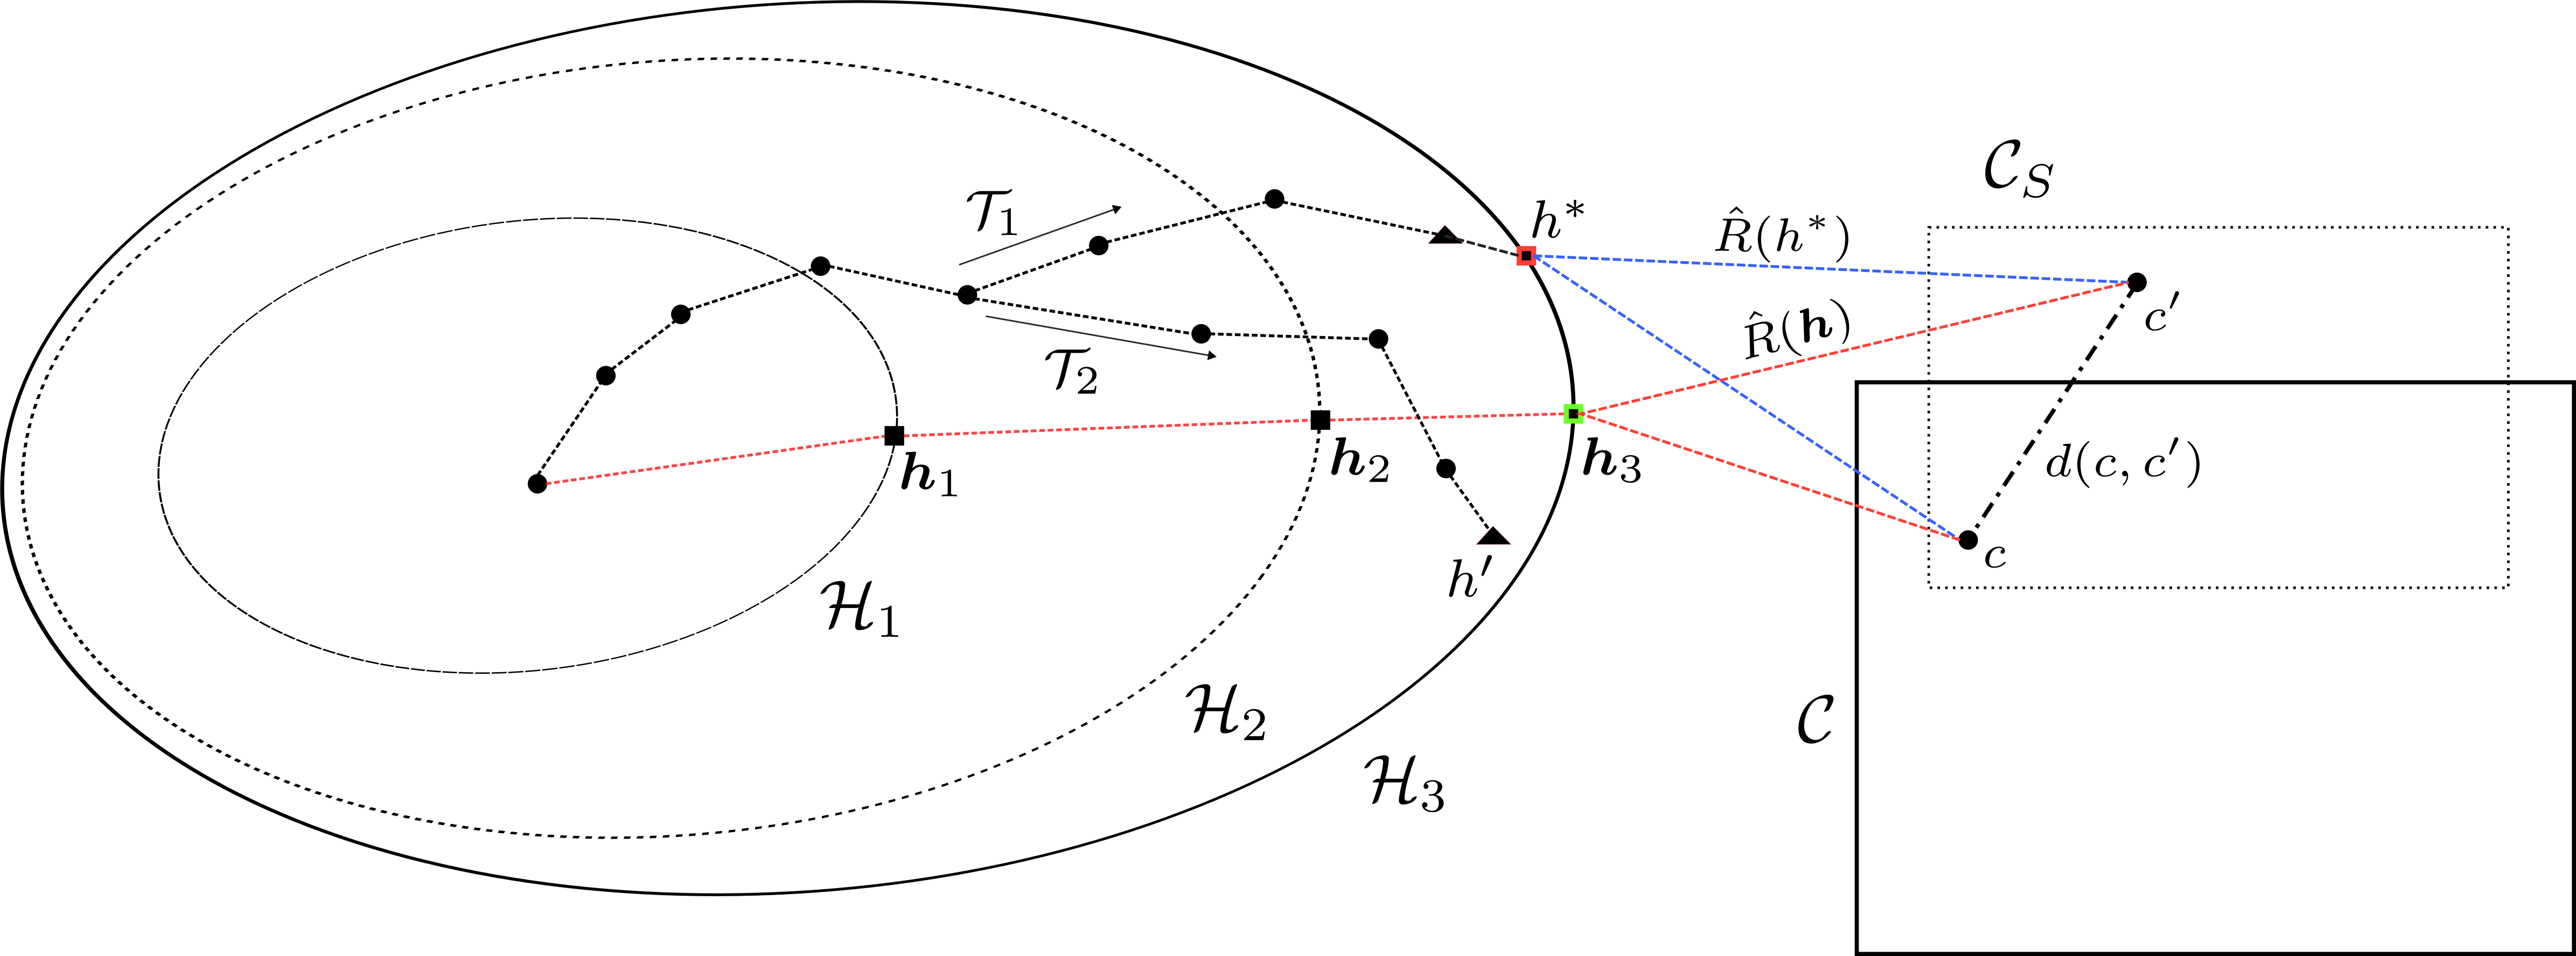
\includegraphics[width=0.9\textwidth]{g10.png}
  \caption{{\small \textbf{Illustrative dynamic of the learning problem.} For an incremental hypothesis space sequence $\mathcal{H}_{1},\mathcal{H}_{2},\mathcal{H}_{3}$, we aim to obtain the procedure $\mathcal{T}$ that would either reach the \textit{generalization solution} $\bm{h}$, or the \textit{empirical solution} $h^{*}$ for a particular hypothesis class, with respect to the concept $c$ and its observed concept $c'$. Model selection hence dictates how an algorithm or procedure than choose the best possible hypothesis to approximate the generalization solution from the empirical solution set. Do notice that here we explicitly state that the data would create a \textbf{proxy concept} that overlaps with the concept class and of some arbitrary `distance' from the true concept by $d(c,c')$. In case the two classes overlap, there still exists the arbitrary distance. Also, we can also observe the intuitive notion of increasing hypothesis class - while it indeed can help in getting closer to the concept class, the somewhat intrinsic property of current learning theory being the relative random procedure class make it probabilistically unstable.}}
  \label{fig:statlearnclassical}
\end{figure}

For fixed $\mathcal{H}$, for fixed and sufficiently large $\mathcal{S}$, and no observation (data) errors, the empirical risk is the generalization risk. These two measures between $h$ and $c$ constitute the learning problem, which can also be separated into both cases - either empirical learning or generalization learning, one to minimize $\hat{R}(h)$, and one to minimize $R(h)$. 

\begin{definition}[Empirical learning problem]
    We present the formal form of the empirical learning. Suppose we have a \textbf{target}, $c\in\mathcal{C}$, where $\mathcal{C}$ is an arbitrary concept class that captures targets of the same type. Suppose we are provided a set of observations $\mathcal{S}$. The problem is to use certain algorithm $\mathcal{A}$ using $\mathcal{S}$, to obtain a hypothesis $h^{*}$ for a fixed $\mathcal{H}$ such that: 
    \begin{equation}\label{eq:lp1}
        R(h^{*}) = \min_{h\in\mathcal{H}} \hat{R}(h) = \min_{h\in\mathcal{H}} \underset{x\sim\mathcal{D}, x\in \mathcal{S}}{\mathbb{E}}\:\ell\{h(x),c(x)\}
    \end{equation} 
\end{definition}

The generalization best $\bm{h}$ is also called in literature as the \textit{Bayes model}, such that it reduces the Bayes risk that is the infimum of the generalization risk, $R^{*}=\inf_{h\in \mathcal{H}}R(h)$. The hypothesis $h^{*}$ is often called the \textit{empirical best}, for it being the minimal, finite hypothesis of the lowest loss evaluation on the entire observation space $\mathcal{S}$. There exists no certified assumption regarding whether $h^{*}$ aligns with the minimal generalization error.

\begin{definition}[Generalization learning problem]
    We present the formal form of the generalization learning problem. Suppose we have a \textbf{target}, $c\in\mathcal{C}$, where $\mathcal{C}$ is an arbitrary concept class that captures targets of the same type. Suppose we are provided a set of observations $\mathcal{S}$. Supposed we have an algorithm $\mathcal{A}$ that for fixed hypothesis space $\mathcal{H}$, \eqref{eq:lp1} holds true. The problem is to use certain algorithm $\mathcal{A}'$ such that, under limited availability, to obtain $\bm{h}$, satisfies: \begin{equation}
        R(\bm{h}) = \min_{h\in \mathcal{H}} R(\bm{h}) \leq \{\epsilon\}, \quad \epsilon > 0 
    \end{equation}
    For a set of risk bounds $\epsilon$. If the setting is deterministic, then there exists $\epsilon=0$. 
\end{definition}

Then, we can partially say that generalization problem is an advancement from empirical solution. As such, empirical solution imposes the observed concept, and not the concept itself. This is reflected in modern machine learning landscape, by modelling the concept as distributions, and then using notions such as KL-divergence to measure such relative disparity. 

These two stages of learning procedure comes of as the intrinsic design of machine learning setting. As opposed to interpolation, where empirical learning problem would have to be put into first priority to achieve the best possible point-through model, machine learning leans on approximation more and a separated criterion that is only visible in the learning setting - the fact that we are using $c'$ to extract $c$. This disparity is exactly the \textbf{generalization problem}, of which is then also the goal of machine learning, to approximate the general solution using the observed solution. One then can ask what is the difference between the two notions, and when we can guarantee that both will `converge' to the same point. The process of \textbf{model selection} is then the procedure that will optimize $h\in \mathcal{H}$ to a given target fixture, such as the empirical best. 

One of the major assumption or observation from the point of the hypothesis class, is that the hypothesis cannot know the generalization error. Thereby, the more efficient and often used procedure/algorithm in training, is then the \textit{empirical risk minimization} (ERM) method, minimizing only the empirical risk to the empirical best; then, certain measures to `generalize' this heuristically is apprehended on the hypothesis. The process of model selection is also the place that we get the concept of \textbf{bias-variance tradeoff}. 
\subsubsection{Uniform convergence}

Suppose that for a concept class $\mathcal{H}$, we can then partition it to $\mathcal{H}=\bigcup_{k\in \mathbb{N}} \mathcal{H}_{k}$ for finite $k$ hypotheses. Assume that they satisfy the uniform convergence (\cite{JMLR:v11:shalev-shwartz10a}): 

\begin{equation}
    \sup_{\mathcal{D}} \underset{S\sim\mathcal{D}^{m}}{\mathbb{E}} \left[ \sup_{h\in\mathcal{H}} [R(h) - R_{S}(h)] \right] \overset{m\to\infty}{\longrightarrow} 0
\end{equation}

This uniform convergence holds for a learning problem, if the empirical risks of hypotheses in the hypothesis class converges to their population risk uniformly, with a distribution-independent rate. The result of this is that a problem then can be considered learnable with the ERM rule, for any given characterization. We state the following definition.

\begin{definition}
    A learning problem is learnable if there exist a learning rule $\mathcal{A}$ and a monotonically decreasing sequence $\epsilon_{cons}(m)$ such that $\epsilon_{cons}(m)\overset{m\to\infty}{\longrightarrow} 0$ and \begin{equation}
        \forall \mathcal{D} , \quad \underset{S\sim\mathcal{D}^{m}}{\mathbb{E}} \left[F(\mathcal{A}(S))-F^{*}\right] \leq \epsilon_{cons}(m) , \quad F^{*} = \inf_{h\in\mathcal{H}} R(h)
    \end{equation}
    A learning rule $\mathcal{A}$ for which this hold is denoted as a universally consistent learning rule. 
\end{definition}

There are certainly a fundamental class of rule or algorithm $\mathcal{A}$ to resolve this particular uniform convergence of classes. One of the major assumption or observation from the point of the hypothesis class, is that the hypothesis cannot know the generalization error. Thereby, one strategy is the \textit{empirical risk minimization} (ERM) method, minimizing only the empirical risk to the empirical best; then, certain measures to `generalize' this heuristically is apprehended on the hypothesis. 

\begin{definition}
    A rule $\mathcal{A}$ is an ERM (Empirical Risk Minimizer), denoted $\mathcal{A}_{ERM}$ if it minimizes the empirical risk $\hat{R}(h)=(1/m)\sum_{c\in\mathcal{C}}\ell(h,c)$, over the observational space $S$, 
    \begin{equation}
        \hat{R}_{S}(\mathcal{A}_{ERM}(S)) = \hat{R}_{S} (h_{S}) = \inf_{h\in\mathcal{H}} \hat{R}_{S}(h) 
    \end{equation}
    Hence, the ERM tries to obtain $\mathrm{ERM}(h') = \argmin_{h\in \mathcal{H}} \hat{R}(h)$. 
\end{definition}

The problem of overfitting still somewhat resides in the setting of the method. Hence, usually, we have an implicit term in addition, called the \textit{regularizer}, of which is as followed. 

\begin{definition}
    A rule $\mathcal{A}$ is an SRM (Structural Risk Minimizer), denoted $\mathcal{A}_{ERM}$ if it minimizes the empirical risk $\hat{R}(h)=(1/m)\sum_{c\in\mathcal{C}}\ell(h,c)$, over the observational space $S$, 
    \begin{equation}
        \hat{R}_{S}(\mathcal{A}_{SRM}(S)) = \hat{R}_{S} (h_{S}) + \lambda r(h)= \inf_{h\in\mathcal{H}} \hat{R}_{S}(h) + \lambda r(h)
    \end{equation}
    of the regularizing term $r(\cdot)$. Hence, the SRM tries to obtain $\mathrm{ERM}(h') = \argmin_{h\in \mathcal{H}} \hat{R}(h)$, while taking into consideration a forcing term $r$, usually defined on the model complexity. 
\end{definition}

In this paper, we would like to presume the ERM method in question as the famous \textit{gradient descent}. We refer to \cite{achlioptas_stochastic_nodate,ruder_overview_2017} for general view of the algorithm, and \cite{zhang_gradient_2019} for a source on particularly gradient descent algorithm on deep learning models. 

\subsection{Overfitting and underfitting}

Following the above framework of statistical probabilistic learning theory, one understanding about the concept of underfitting and overfitting (similar to \cite{gareth_james_introduction_2013}) can be reached, using the notion of \textit{partitioning} of observation space. We can define the heuristic for better definition, as followed. 

\begin{definition}[Heuristic empirical risk]
  Given a dataset $\mathcal{S}$ of size $m$, supposedly of the concept $c\in \mathcal{C}$, and the hypothesis $h\in \mathcal{H}$, then the \textbf{heuristic empirical risk} take a partitioning $k<m$ with $k/m\geq 1/2$, hence defining the heuristic empirical loss on $k$, denoted $\hat{R}_{k}(h)$. 
\end{definition}

\begin{definition}[Heuristical generalization risk]
  Given a dataset $\mathcal{S}$ of size $m$, supposedly of the concept $c\in \mathcal{C}$, and the hypothesis $h\in \mathcal{H}$. Fixed $\hat{R}_{k}(h)$, for the final optimization of algorithm $\mathcal{A}$, then the \textbf{heuristic generalization risk} take the remaining 2-partition of portion $p=k-m$, hence defining the heuristic generalization loss on $p$, denoted $\hat{R}_{p}(h_{\mathcal{A}})$. 
\end{definition}
The two heuristic definition however, can be noted to not be equal to the true generalization risk - empirical risk pair in reality. Nevertheless, one can then define overfitting and underfitting in such manner. 
\begin{definition}[Underfitting]
  A model $h$ is called \textbf{underfitting} if for a constant $\epsilon > 0$ chosen for the setting, then $\hat{R}_{k}(h)>\epsilon$, $\hat{R}_{p}(h_{\alpha})> \epsilon$ over the entire observation space. 
\end{definition}
Usually, underfitting is defined to be such that test error is smaller than training error partition, however, we do not think that is a good definition. Especially since, at least in this setting, the empirical error under algorithm $\mathcal{A}$ is reduced to the representative smallest error that $\mathcal{A}$ can achieve on that particular model, within particular setting of $h$, then come the heuristic generalization error. Considering also that $k/m\geq 1/2$, that is, at least the training partition is half of the observation set, then only under very specific case will $\hat{R}_{p}(h_{\alpha})$ be smaller than $\hat{R}_{k}(h)$, statistically speaking. Thence this line of thought also reinforces the idea that both of them will be larger than the threshold $\epsilon$. Usually, heuristically, this threshold of error is $0.3$, normalized. Next, we define the notion of overfitting. 

\begin{definition}[Overfitting]
  A model $h$ is called \textbf{overfitting} if there exists a specific constant $\epsilon>0$ chosen for the setting, such that $\hat{R}_{k}(h)<\epsilon$, $\hat{R}_{p}(h_{\alpha})> \epsilon$ over the entire observation space.
\end{definition}
Namely, this mean that the static learning makes the generalization error worse. This draws the analogy of the student - studying explicitly for the past paper tests, yet unaware of the larger margin of questions in the large set of the test paper pool, leading to subpar performance. Similarly, overfitting is theorized to be fitting too fit to the reduced observation space - hence when it comes to the generalization observation space, it fails within such heuristic. The notion works on the mask of the risks, $\hat{R}_{k}$ and $\hat{R}_{p}(h_{\alpha})$. 

\subsection{Bias-variance tradeoff}

In classical sources, \cite{gareth_james_introduction_2013,goodfellow2016deep,STL_Hajek_Maxim_2021,10.5555/2371238,10.5555/2621980}, bias-variance tradeoff is a classical principle used in the categorization of technique called \textit{model selection}. Specifically, this refers to the progress of choosing the best predictor $h^{*}$ that minimize the generalization error that is the main goal of a particular machine learning model, during the process of training and inference. Originally, the theory that bias and variance often come in to conjunction is \textbf{Estimation theory}, of which there exists an estimator $\hat{\theta}$ that use a set of observations, to estimate the concept, or the underlying mechanics of certain system that outputted the observation set, by the \textbf{probabilistic perspective} - that is, it is governed by appearance by an independently and identically distributed process of parameterized probability $\theta\in \Theta$. Here, parameterized means being expressed by a set, often finite, of parameters, by \cite{LehmannCasella_theory_1998,liam_statistics_2005}. It is only when \cite{6797087} introduced it to machine learning that we have an equivalent structure that is similar to bias-variance in machine learning. 

\subsubsection{Precursor (Geman et al., 1992)}

The original definition of bias-variance tradeoff by \cite{6797087} is first constructed using the means-square error, which is regarded as a normal measure in the real encoding space. Their approach is to justify bias-variance via decomposition of the loss function $\ell$, for such to find an alternative reasonable form of such loss landscape. Suppose of a regression problem to construct a hypothesis function $f(x)$ from $(x_{1},y_{1},\dots,x_{N},y_{N})$ for the purpose of generalization - that is, predicting unseen variational values for different pair $(x_{j}, \mathord{?})$ such that $\mathord{?}=y_{j}+\epsilon$ for a conceivable implicit error. To be explicit about the relation of this problem, or $f$ on the given data $\mathcal{D}=\{(x_i, y_i)\mid i \leq N\}$, denote $f(x;\mathcal{D})$ instead of $f$, the natural mean-square measure as a predictor is: 
\begin{equation}
    \mathcal{M}(f,y) = \mathbb{E} \left[((y-f(x;\mathcal{D})))^{2}\mid x, \mathcal{D}\right] 
\end{equation} for $\mathbb{E}[\cdot]$ the expectation wrt to a distribution $P$. Decomposing the right-hand side, we have: 
\begin{equation}
    \mathcal{M}(f,y) = \mathbb{E} \left[((y-f(x;\mathcal{D})))^{2}\mid x, \mathcal{D}\right] = \mathbb{E}\left[(y-\mathbb{E}[y\mid x])^{2}\mid x,\mathcal{D}\right] + (f(x;\mathcal{D})-\mathbb{E}[y\mid x])^{2}
\end{equation}
Here, $\mathbb{E}\left[(y-\mathbb{E}[y\mid x])^{2}\mid x,\mathcal{D}\right]$ does not depend on $\mathcal{D}$, but simply the statistical variance of $y$ given $x$. The term $(f(x;\mathcal{D})-\mathbb{E}[y\mid x])^{2}$ is considered a natural measure of effectiveness on $\mathbb{R}^{n}$ as a singular predictor of $y$. Now, for $\mathbb{E}_{\mathcal{D}}\left[(f(x;\mathcal{D})-\mathbb{E}[y\mid x])^{2}\right]$ which depends on the training set $\mathcal{D}$ in its computation, is decomposed into the form of \textit{bias-variance decomposition} terms, by derivation: 
\begin{equation}
    \begin{split}
        \mathbb{E}_{\mathcal{D}} \left[(f(x;\mathcal{D})-\mathbb{E}[y\mid x])^{2}\right] & = \underbrace{\left\{ \mathbb{E}_{\mathcal{D}}[f(x;\mathcal{D})] - \mathbb{E}[y\mid x] \right\}^{2}}_{\text{bias term}} + \underbrace{\mathbb{E}_{\mathcal{D}} \left\{(f(x;\mathcal{D})- \mathbb{E}_{\mathcal{D}}[f(x;\mathcal{D})])^{2}\right\}}_{\text{variance term}}
    \end{split}
\end{equation}

We summarize this in the following statement. 

\begin{theorem}[Bias-variance decomposition]
    Suppose the model $f(x;\mathcal{D})$ for the data $\mathcal{D}=(x_i, y_i)$ and its parameter $x$ is defined. For $y_{i}$ of the target concept's responses $y$, and consider a regression problem with the loss measure $\mathcal{M}(f,y)$ of mean squared risk, the following statement is true: \begin{equation}
        \mathbb{E}\big[\mathcal{M}(f,y)\big] = \mathcal{B}(f,y) + \mathcal{V}(f,y) + \mathbb{E}\Big[\mathbb{E} \left[((y-f(x;\mathcal{D})))^{2}\mid x, \mathcal{D}\right]\Big]
    \end{equation}
    for $\mathbb{E}[\:\cdot\mid x, \mathcal{D}]$ any expression with dependencies on $x$ and $\mathcal{D}$. The bias and variance term is subsequently expressed by 
    \begin{align}
        \mathcal{B}(f,y) = \underbrace{\left\{ \mathbb{E}_{\mathcal{D}}[f(x;\mathcal{D})] - \mathbb{E}[y\mid x] \right\}^{2}}_{\text{bias }}, \quad \mathcal{V}(f,y) =\underbrace{\mathbb{E}_{\mathcal{D}} \left\{(f(x;\mathcal{D})- \mathbb{E}_{\mathcal{D}}[f(x;\mathcal{D})])^{2}\right\}}_{\text{variance}}
    \end{align}
\end{theorem}

\begin{SCfigure}[0.5][htb]
  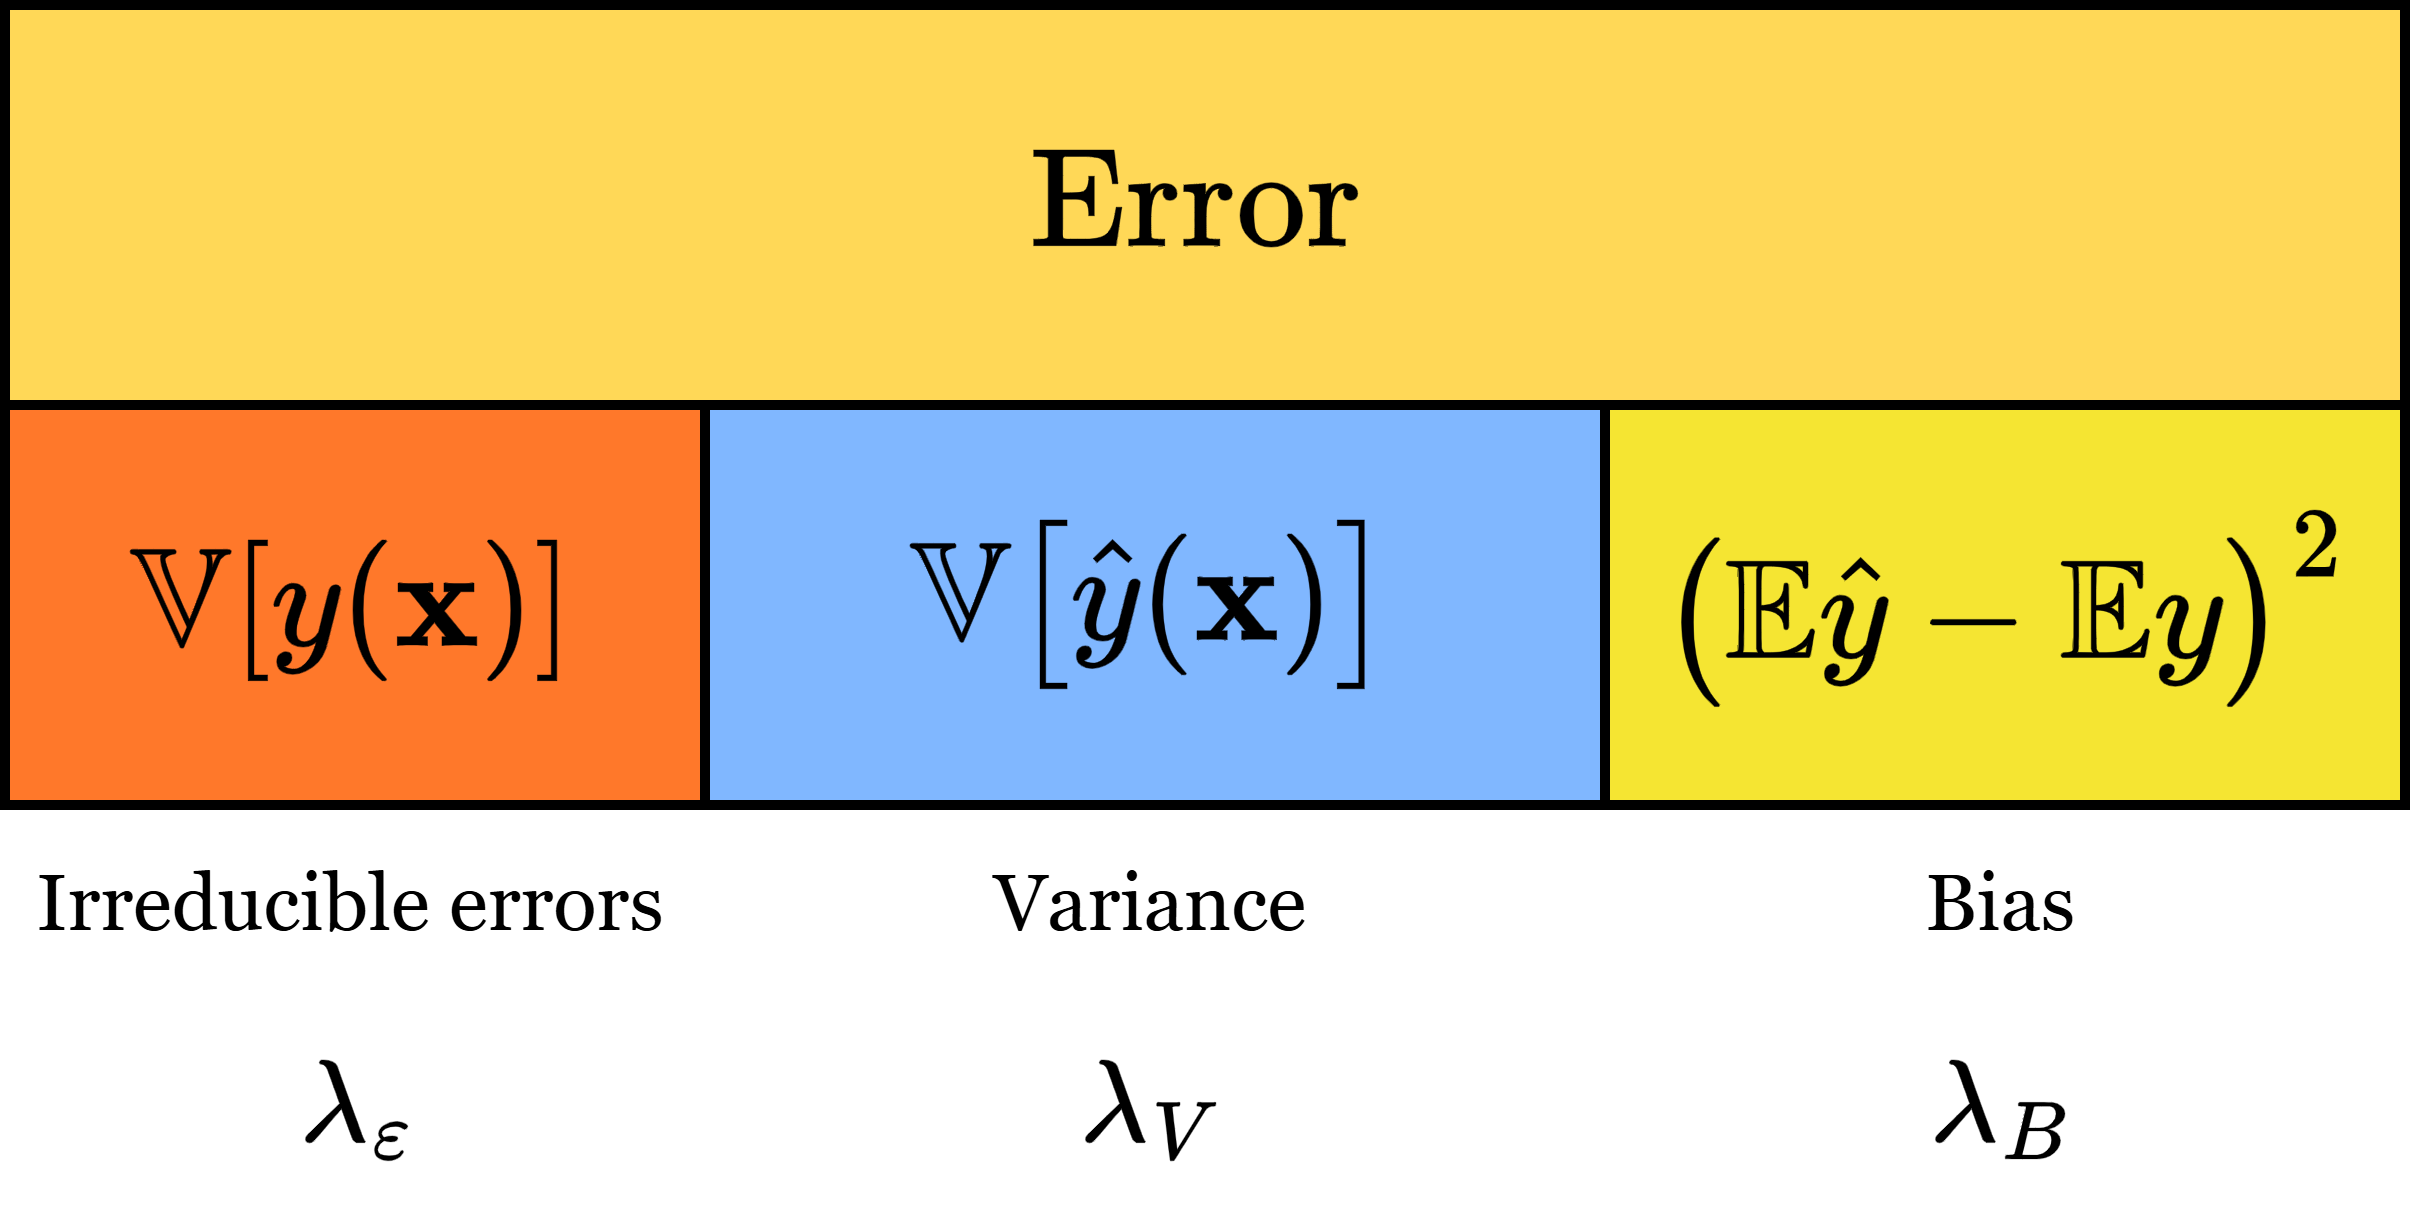
\includegraphics[width=0.5\textwidth]{error_decomposition.png}
  \caption{\textbf{Decomposition of the error term into 3 parts}. Respectively, the irreducible error $\mathbb{V}[y(\mathbf{x})]$, the variance (blue) and the bias (dark yellow). All of them are assumed to take up 100\% of the error observed in such composition. The proportion is included using the three coefficient $\lambda_{\epsilon},\lambda_{V},\lambda_{B}$ where $\lambda_{\epsilon}+\lambda_{V}+\lambda_{B}=1$.}
\end{SCfigure}

The above decomposition principle is often expressed into a form where there exists the intrinsic noise \cite{brown2024biasvariance}: 
\begin{equation}
    \begin{split}
        \mathbb{E}_D \left[ \mathbb{E}_{xy} \left( y - \hat{f}(x) \right)^2 \right]
        &= 
         \mathbb{E}_x \left[ \left( y^* - \mathbb{E}_D[\hat{f}(x)] \right)^2 \right]
        + \mathbb{E}_x \left[ \mathbb{E}_D \left( \hat{f}(x) - \mathbb{E}_D[\hat{f}(x)] \right)^2 \right] \\
        &+ \mathbb{E}_{xy} \left[ \left( y - y^* \right)^2 \right]
    \end{split}
    \end{equation}
In all, almost all representation of bias-variance decomposition are the same. For simplicity of notation, we adopt the similar form in the standard case of the paper \cite{adlam2020understandingdoubledescentrequires}: 
\begin{equation}
    \E \qa{\hat{y}(\bfx)-y(\bfx)}^2 = \pa{\E\hat{y}(\bfx) - \E y(\bfx)}^2 + \V\qa{\hat{y}(\bfx)} + \V\q{y(\bfx)}
\end{equation}
A main common theme of criticism toward bias-variance tradeoff is the fact that the decomposition is much more general, and intrinsic for the class of \textit{mean squared loss}. However, when considering the naturalness of an error measure and then its direct applicant, mean square error on real space of sufficient support and measure comes of as a very natural choice of an error measure, at least in consideration of the regression setting; for that, we then can also define classification as another top-layer above a regression's similar real continuous space, i.e. a decision layer. Furthermore, it can also be shown \cite{brown2024biasvariance,PfauBregmanDivergence} that it also holds for the class of Bregman divergence measure. 

What does the decomposition say about model selection principle in general? In general, bias-variance is typically presented of its decomposition only, and the asymptotic prediction of its behaviours. In fact, one of the reason that it became the rule-of-thumb for ML practitioner, as well as generally statistical learning (\cite{lafon_understanding_2024} provides a quite rigorous treatment of bias-variance tradeoff in the section on statistical learning theory) solidify the trade-off as a particular model selection principle. Generally, this tradeoff can be summarized as followed: 
\begin{theorem}[Bias-variance tradeoff]
    For the expected loss of any given hypothesis $h$, the bias $\mathcal{B}(f,y)$ and variance $\mathcal{V}(f,y)$ is inversely proportional, that is, $\mathcal{B}(f,y)\propto \lambda^{-1} \mathcal{V}(f,y)$ for some proportionality $\lambda$ that may or may not be constant. In the most general case possible, $\lambda = -1$ on the entire error range. 
\end{theorem}

The tradeoff is then of inverse proportionality. Indeed, statistically, we have such tradeoff on a statistical framework in a more concrete sense. For the bias to increase, variance will increase, of which the criterion is inverse - we would like to have more bias but lower variance, and vice versa, according to such theory. 

\subsubsection{Expansion and variations}

The bias-variance decomposition and tradeoff is not general. Indeed, works, by \cite{6797087,sharma_bias-variance_2014,domingos_unifeid_2000,adlam2020understandingdoubledescentrequires,yang_rethinking_2020} and more all attempted to reconstruct and reformulate bias-variance, and it did leave out a picture of uncertainty regarding the concept. Specifically, there are certainly different way to do the bias-variance decomposition, as classified in \cite{adlam2020understandingdoubledescentrequires} paper. Some of this are particularly specialized in \textit{neural network} training, basing on the main structure of modern machine learning in neural network formalism. 
\begin{enumerate}[leftmargin=1cm,itemsep=2pt,topsep=1pt]
    \item \textbf{Semiclassical approach}: The semiclassical approach is fairly simple. We can rewrite to another variation of the classical approach to be \begin{equation}
        \underset{h\in\mathcal{H}}{\mathbb{E}[\ell(h)]} = \mathbb{E}_{x}\mathbb{E}_{\epsilon}\left[\hat{y}(x)-y(x)\right]^{2} = \mathbb{E}_{x}\left(\mathbb{E}_{\epsilon}[\hat{y}(x)]-y(x)\right)^{2} + \mathbb{E}_{x}\mathbb{V}_{\epsilon}\left[\hat{y}(x)\right]  
    \end{equation}
    and instead, consider the \textit{structural conformation} of the decomposition, or rather, taking the expectation within $\theta\in \Theta$ of the structural description of $h\in\mathcal{H}$. Then, we shall have 
    \begin{equation}
        \underset{h\in\mathcal{H}}{\mathbb{E}_{\mathrm{SC}}[\ell(h)]} = \mathbb{E}_{x}\mathbb{E}_{\theta}\mathbb{E}_{\epsilon}\left[\hat{y}(x)-y(x)\right]^{2} = \mathbb{E}_{x}\mathbb{E}_{\theta}\left(\mathbb{E}_{\epsilon}[\hat{y}(x)]-y(x)\right)^{2} + \mathbb{E}_{x}\mathbb{E}_{\theta}\mathbb{V}_{\epsilon}\left[\hat{y}(x)\right]
    \end{equation}
    Do note that the order matters, since the expectation can be constant of a given ordering. And expected value over constant is just the constant. 
    \item \textbf{Symmetric decomposition}: This approach is fairly difficult, we refer to the paper itself of its own justification on the decomposition. The symmetric decomposition relies on the shape of the input, $\mathcal{X}=\{P,D,\epsilon\}$, of which you can remove the $\epsilon$ term and retain some decomposition on $P$ and $D$ per distribution. 
\end{enumerate}

\subsubsection{Generalized decomposition}

According to \cite{domingos_unified_aaai_2000,domingos_unified_2000}, the bias-variance decomposition can usually be treated as being controlled by three factor error, with their respective coefficients $\lambda=(\lambda_{1},\lambda_{2},\lambda_{3})$ for such: 
    \noindent 
    \begin{equation*}
        \begin{split}
            \mathbb{E}_{\mathcal{D}} \left[d((f,\mathbb{E}[y\mid x])\right] & = \lambda_{1} \mathrm{Bias}(f,y) + \lambda_{2}\mathrm{Var}(f,y)+ \lambda_{3}\epsilon(\mathcal{D})\\ 
            & = \lambda_{1}\underbrace{\left\{ \mathbb{E}_{\mathcal{D}}[f(x;\mathcal{D})] , \mathbb{E}[y\mid x] \right\}}_{\text{bias term}} +\lambda_{2} \underbrace{\mathbb{E}_{\mathcal{D}} \left\{(f(x;\mathcal{D}), \mathbb{E}_{\mathcal{D}}[f(x;\mathcal{D})])\right\}}_{\text{variance term}} +\underbrace{\lambda_{3}\epsilon}_{\text{irreducible error}}
        \end{split}
        \end{equation*}
where $\epsilon(\mathcal{D})$ is the irreducible error of the system, depends (theoretically) on the intrinsic imperfection of the dataset $\mathcal{D}$. This method of which the bias-variance-irreducible error are `fit' into the total error by three coefficients $\lambda_{1},\lambda_{2},\lambda_{3}$ instead. This does not only scale up the B-V-IE triplet, but also leaves out the inexplainable gap between the scaling, and the actual normal measure. 

\subsubsection{Approximation-Estimation tradeoff}

Another closely related notion to bias-variance is the concept of approximation-estimation tradeoff. We refer to \cite{10.5555/2371238,lafon_understanding_2024} for some analysis and mentions. 

Let $\mathcal{H}$ be a family of functions mapping $\mathcal{X}\to\{1,-1\}$. This is the particular case of \textbf{binary classification}, in which can be straightforwardly extended to different tasks and loss functions. The \textit{excess error} of a hypothesis $h\in\mathcal{H}$, is the difference between its error $R(h)$ and the Bayes error $R^{*}$. This can be decomposed to be the following: 

\begin{equation}
    R(h) - R^{*} = \Big( R(h) - \inf_{h\in \mathcal{H}} R(h) \Big) + \Big( \inf_{h\in \mathcal{H}} R(h) - R^{*} \Big)
\end{equation}

The first bracket contains the \textbf{estimation error}, and the second bracket contains what is called the \textbf{approximation error}. The estimation error depends on the hypothesis $h$ selected. It measures the error of $h$ with respect to the infimum of the error achieved by hypotheses in $\mathcal{H}$, or that of the best-in-class hypothesis $h^{*}$ when that infimum is reached. The approximation error measures how well the Bayes error can be approximated using $\mathcal{H}$. It is a property of the hypothesis set $\mathcal{H}$, a measure of its richness. 

Model selection consists of choosing $\mathcal{H}$ with a favourable trade-off between the approximation and the estimation error. However, in the most general case, this will be done, but not in practice, as it requires the underlying distribution $\mathcal{D}$ to be known to determine $R^{*}$, which is not possible. In contrast, the estimation error can be bounded, or can be analysed, using particular metric and analysis. 

Is however, worth to note that bias-variance and approximation-estimation have a very complicated relationship, for example, in \cite{brown2024biasvariance} shown that they are indeed not the same, and is in fact two different decomposition, where one is the others' component.

\subsection{Double descent}

Nevertheless, of bias-variance and the analogous statistical learning theory concept, the target is the same. It is the dilemma of which is presented in \textbf{Occam's razor}, for choosing the sufficient model of good complexity, or bias, for tradeoff of its generalization ability, or variance. Then there must exist a sweet spot between the axis of bias and variance, since they are as exhibited above inversely proportional to each other. However, double descent seemingly broke the status quo, and insists on an interesting phenomenon - under the same setting, if we `crank' the complexity high enough, we will then reach a point then called the \textbf{interpolation threshold}, such that the trend reverse and the error rate, instead of being theorized to go up, goes down to a certain line of lower bound. 

The first identification of the double descent phenomena dated back to the paper of Belkin - \cite{belkin_reconciling_2019}, in which the title is literally "reconciling" modern machine learning practice and the bias-variance tradeoff. In modern machine learning practice, or state-of-the-art developments, models are now bigger than ever. If to notice, we will see that currently models are inherently large, for example, a normal large language model will have from 900 millions (900M) to a few billions, for example 10 billions (10B) parameters. That is not taking into account the overall dynamics and structure of the model, which dictates the operating range and efficiency of the model itself. These model, based on the neural network architecture are somewhat trained to exactly fit (or interpolate) the data, almost certainly so that it turn from a prediction setting to an estimation setting. By statistical learning theory, this would be considered overfitting, and yet, they often obtain very high accuracy on test data.

\begin{figure}[htb]
    \centering
    \begin{tabular}{cc}
    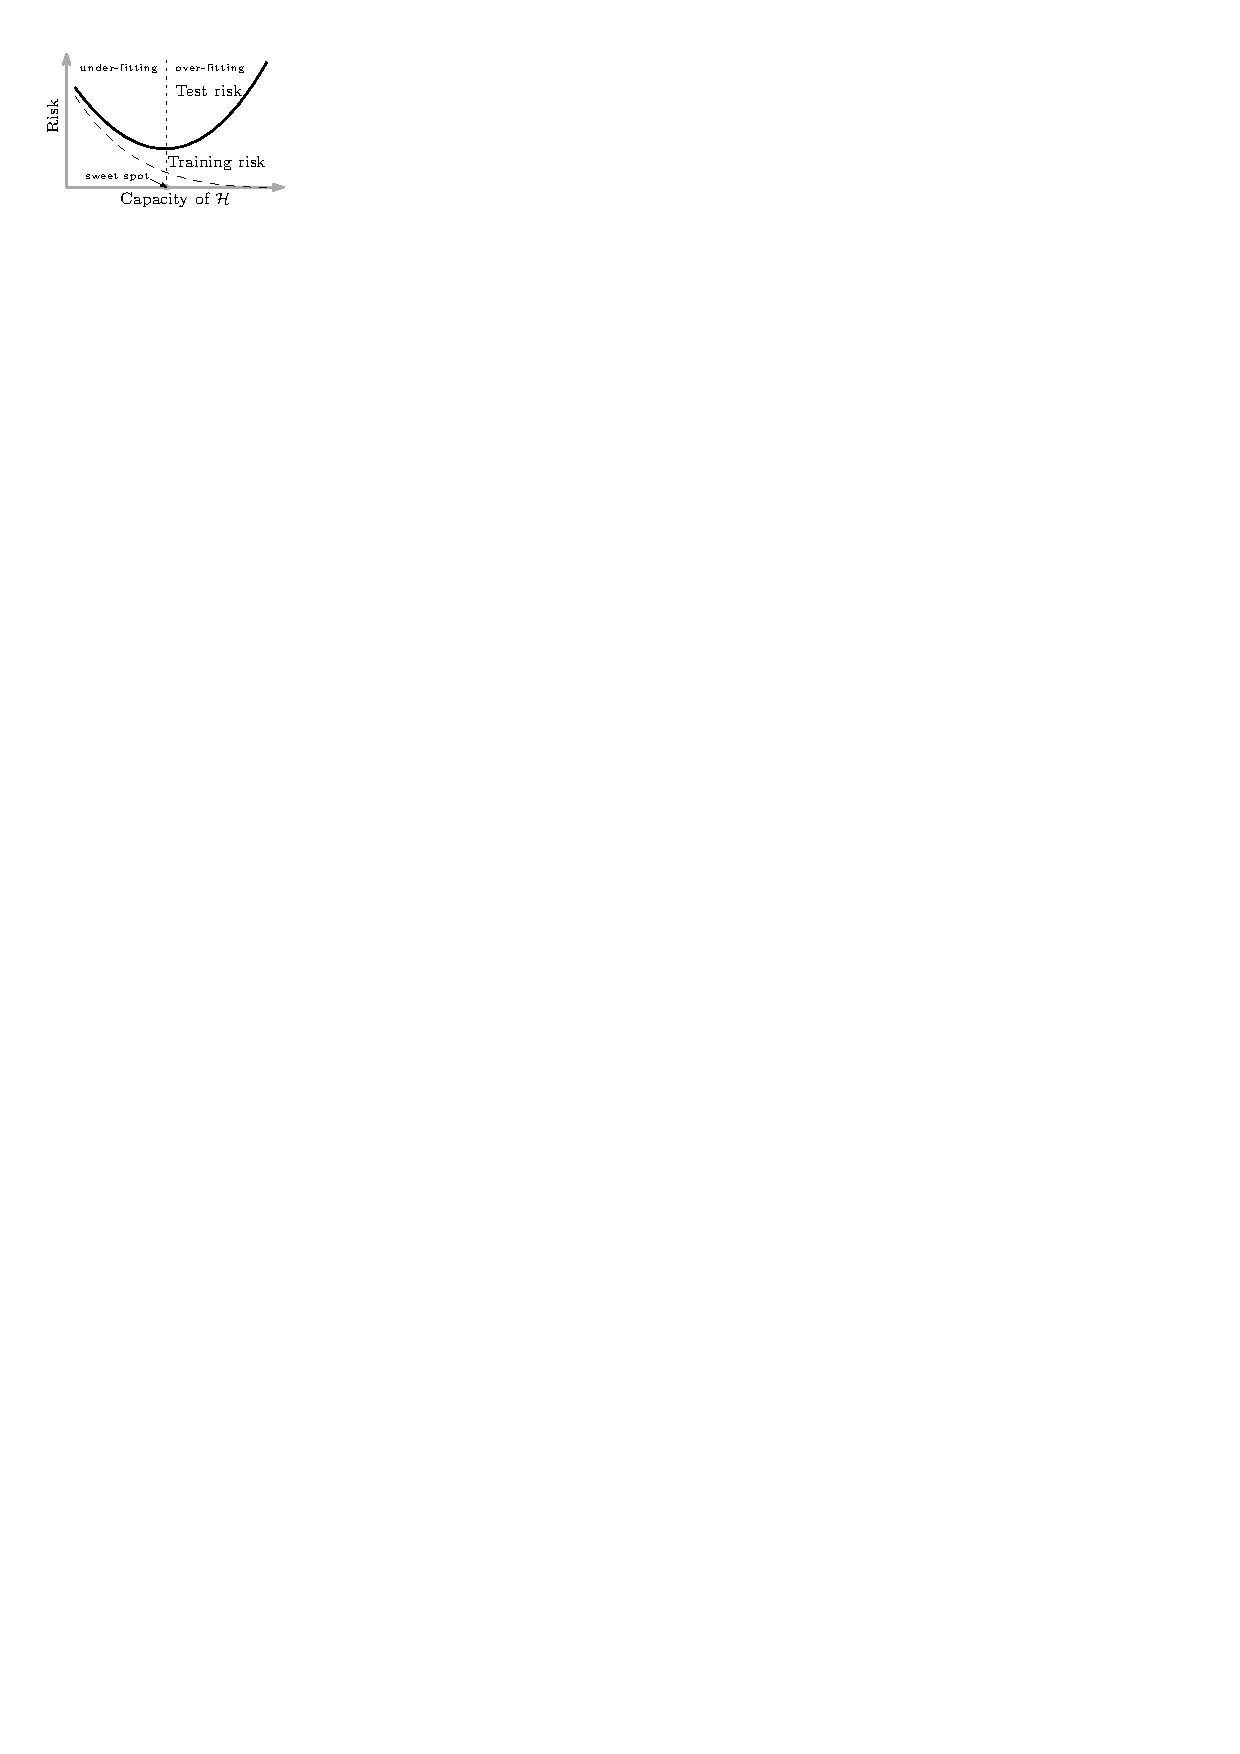
\includegraphics[height=0.13\textheight]{pdf/u-shaped.pdf} &
    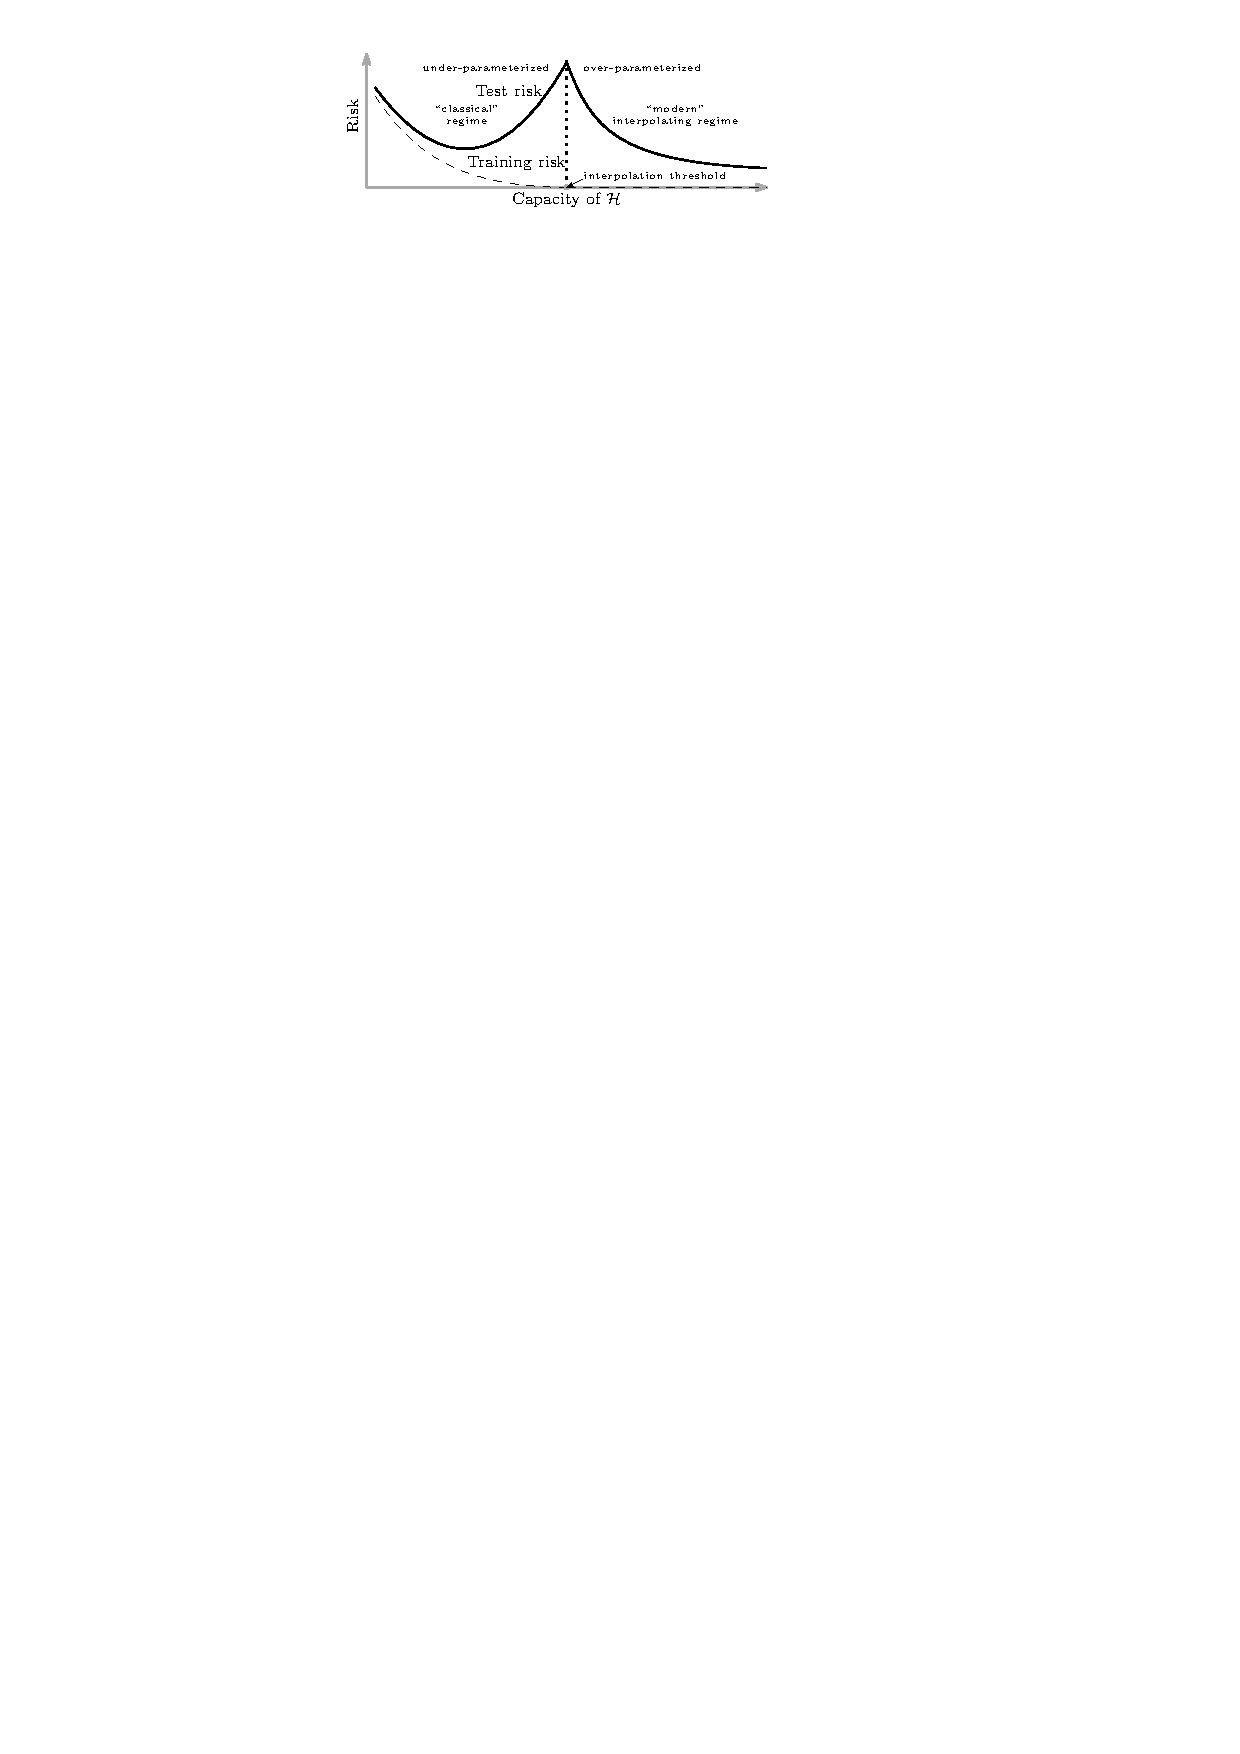
\includegraphics[height=0.13\textheight]{pdf/doubledescent.pdf} \\
    {\bf (a)} & {\bf (b)}
    \end{tabular}
    \caption{{\bf Curves for training risk (dashed line) and test risk (solid line).}
      ({\bf a}) The classical \emph{U-shaped risk curve} arising from the bias-variance trade-off.
      ({\bf b}) The \emph{double descent risk curve}, which incorporates the U-shaped risk curve (i.e., the ``classical'' regime) together with the observed behaviour from using high capacity function classes (i.e., the ``modern'' interpolating regime), separated by the interpolation threshold.
      The predictors to the right of the interpolation threshold have zero training risk. Reproduced from \cite{belkin_reconciling_2019}.}
    \label{fig:double-descent}
\end{figure}

The main finding that Belkin found is a pattern for how the apparent performance on unseen data depends on model capacity and the mechanism underlying the emergence of double descent. When function class capacity is below the "interpolation threshold", learned predictors exhibit the classical $U$-shaped curve from Figure~\ref{fig:double-descent}. The `modern' interpolating regime marks the opposite trend to the right, where the risk starts to decrease up to a lower bound, which then can be called the \textit{optimal descent bound}. 

\blockquote[\cite{belkin_reconciling_2019}]{The bottom of the $U$ is achieved at the sweet spot which balances the fit to the training data and the susceptibility to over-fitting:
to the left of the sweet spot, predictors are under-fit, and immediately to the right, predictors are over-fit.
When we increase the function class capacity high enough (e.g., by increasing the number of features or the size of the neural network architecture), the learned predictors achieve (near) perfect fits to the training data---i.e., interpolation.
Although the learned predictors obtained at the interpolation threshold typically have high risk, we show that increasing the function class capacity beyond this point leads to decreasing risk, typically going below the risk achieved at the sweet spot in the ``classical'' regime.}

At this point, we would like to also clarify the term interpolation threshold in this case. Usually, under the pretext of overfitting and underfitting, interpolation threshold means the following: 
\vspace{2mm}

\begin{definition}[Interpolation threshold]
    Assuming a typical supervised learning setting, for a hypothesis $h$ within class structure $\mathcal{H}$, and a supposed concept $c$ of the class $\mathcal{C}$. Suppose $[X,Y]\subset c\in \mathcal{C}$ being the dataset, or \textit{observable space} of $c$ on which $h$ is tested on. Under the \textbf{empirical generalization learning} procedure, partitioning $[X,Y]$ into $[X,Y]_{1}$ and $[X,Y]_{2}$, for error evaluated on the first set, $\hat{R}_{1}(h)$ called training error, and the second set, $\hat{R}_{2}(h)$ called test error, with optimization applied on the first set, then evaluated statically on the second, the \textbf{interpolation threshold} with respect to a particular complexity measure of $h$, $\mathcal{M}(h)$, is the point $\mathcal{M}_{0}(h)$ where it is possible for $\hat{R}_{1}(h)/\hat{R}_{1}(h)\approx 1$, for $\hat{R}_{1}(h)\ll \epsilon$, $\hat{R}_{2}(h)\ll \epsilon$, with $\epsilon \geq 0$. 
\end{definition}

This basically means that what is learnt, with respect to the model complexity that gauge \textit{how much} and \textit{what} the model can learn, perfectly fits the concept $c$ itself, from the observation space on its own. We can say that the observation space is \textit{fully representative} of the concept class, and the concept class is then fully realized by the model. Such point where that is possible, or there then such behaviour is possible, is called the interpolation point. The definition relies on the statement `where it is possible', hence it still, does not give us a particularly sound notion on to how and what constitute such possibility. The term empirical generalization learning comes from the fact that the procedure in practice of estimating and optimizing train-test-validation set in itself, is an imperfect empirical approximation of generalization testing. While the fact that we cannot gauge generalization error, in a purely blind black-box setting is settled (\cite{10.5555/2371238,10.5555/2930837,10.5555/2621980}), the method is then to try to mimic such by using generalization-via-hidden observations. To facilitate this, deliberately, the empirical learning procedure is only dynamic during training session, and static throughout the whole testing and validation testing section, and further on. 

By default, in general theory, such interpolating point is dangerous. Not only because it is inherently difficult to know exactly what the dataset constitute, whether it is actually representative of the concept that gives rise to it, or the structural information, noises, and interferences in between. It is hence impossible, to a certain point, to truly know the effectiveness of the model beside interpolating the current dataset which forms the observable details. 

Another prominent discovery to look at is \cite{nakkiran_deep_2019}, on the double descent of deep learning models. The paper serves as the first observation upon which double descent is observed on modern, deep learning theoretic models, especially complex one like Transformer or ResNet networks. 

\begin{figure}[htb]
    \centering
    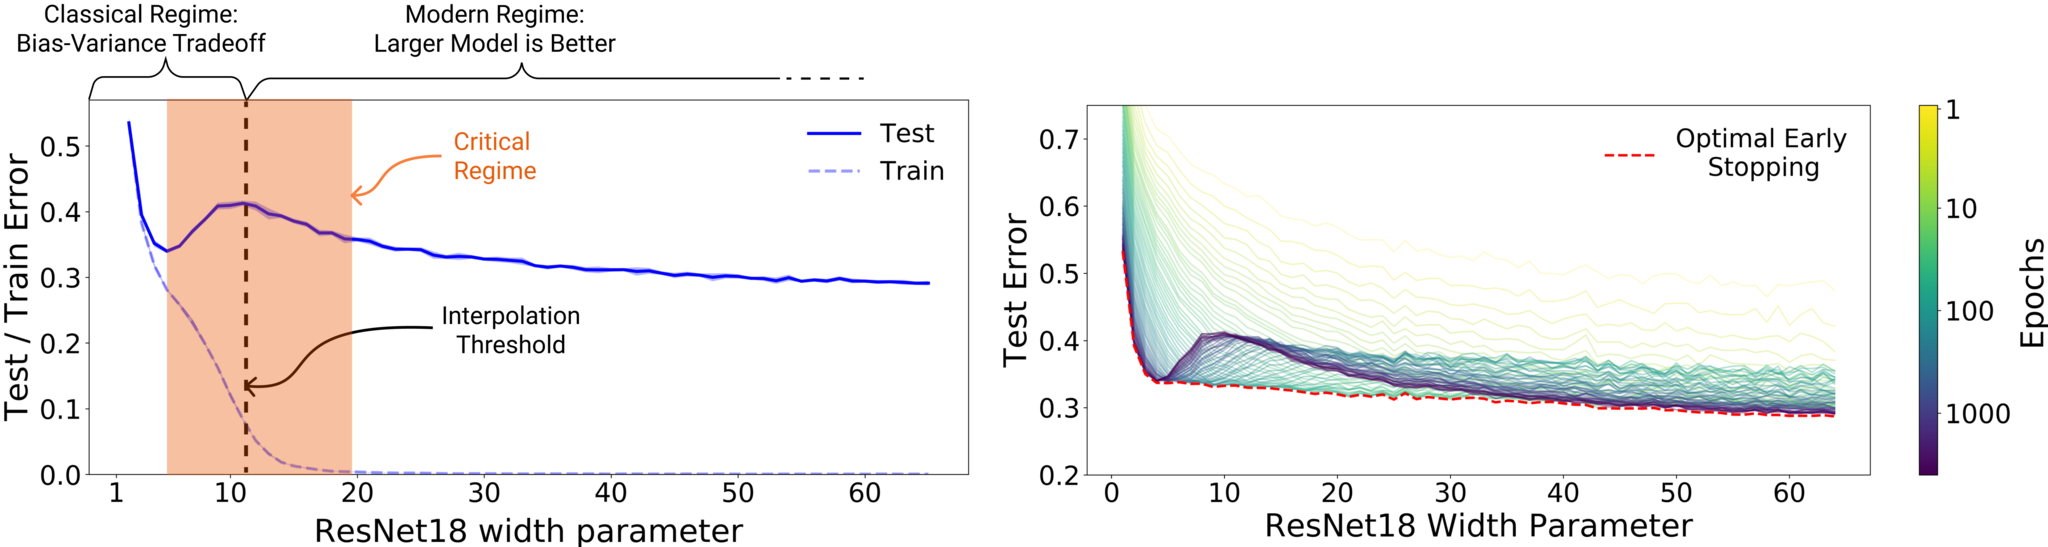
\includegraphics[width=1\textwidth]{media/errorvscomplexity.png}
    \caption{{\bf Left:} Train and test error as a function of model size,
    for ResNet18s of varying width 
    on CIFAR-10 with 15\% label noise.
    %In the under-parameterized regime, test error follows
    %the behavior predicted by classical statistical learning theory, but in the overparameterized regime (once training error is approximately zero),  the test error undergoes a ``second descent'' and decreases as model size increases. The shaded region represents the critically parameterized regime where the transition from under- to over-parameterization occurs. 
    {\bf Right:}
    Test error, shown for varying train epochs.
    %The dashed red line shows that with optimal early stopping double descent is not observed.
    % All models are ResNet18s of varying width,
    % trained on CIFAR10 with 15\% label noise
    All models trained using Adam for 4K epochs.
    %, and plotting means and standard-deviations from 5 trials with random network initialization.
    The largest model (width $64$) corresponds to standard ResNet18. Resued from \cite{nakkiran_deep_2019}.
    %    \ptodo{point out that interpolation point for second plot is plotted in the ocean plot}
    }
    \label{fig:errorvscomplexity}
\end{figure}

\begin{figure}[htb]
\centering
\begin{minipage}{.512\textwidth}
  \centering
  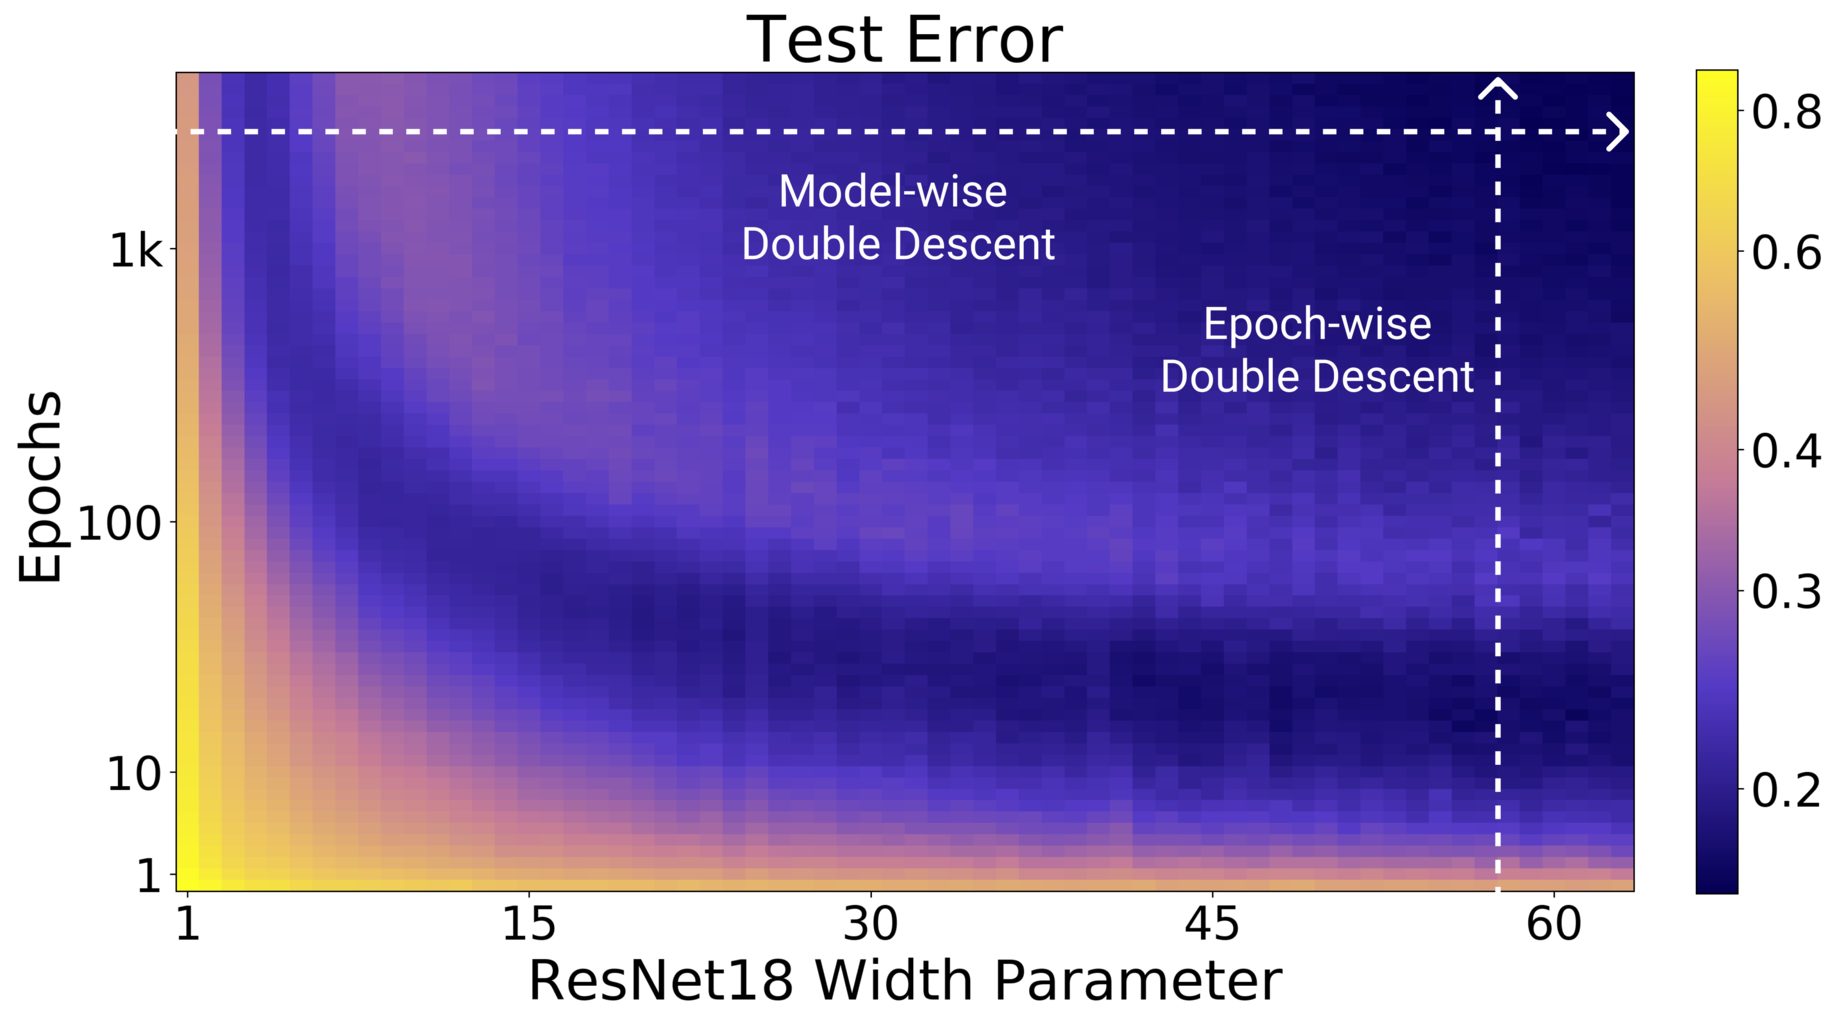
\includegraphics[width=1\textwidth]{media/Intro-ocean-test.png}
\end{minipage}%
\begin{minipage}{.488\textwidth}
  \centering
  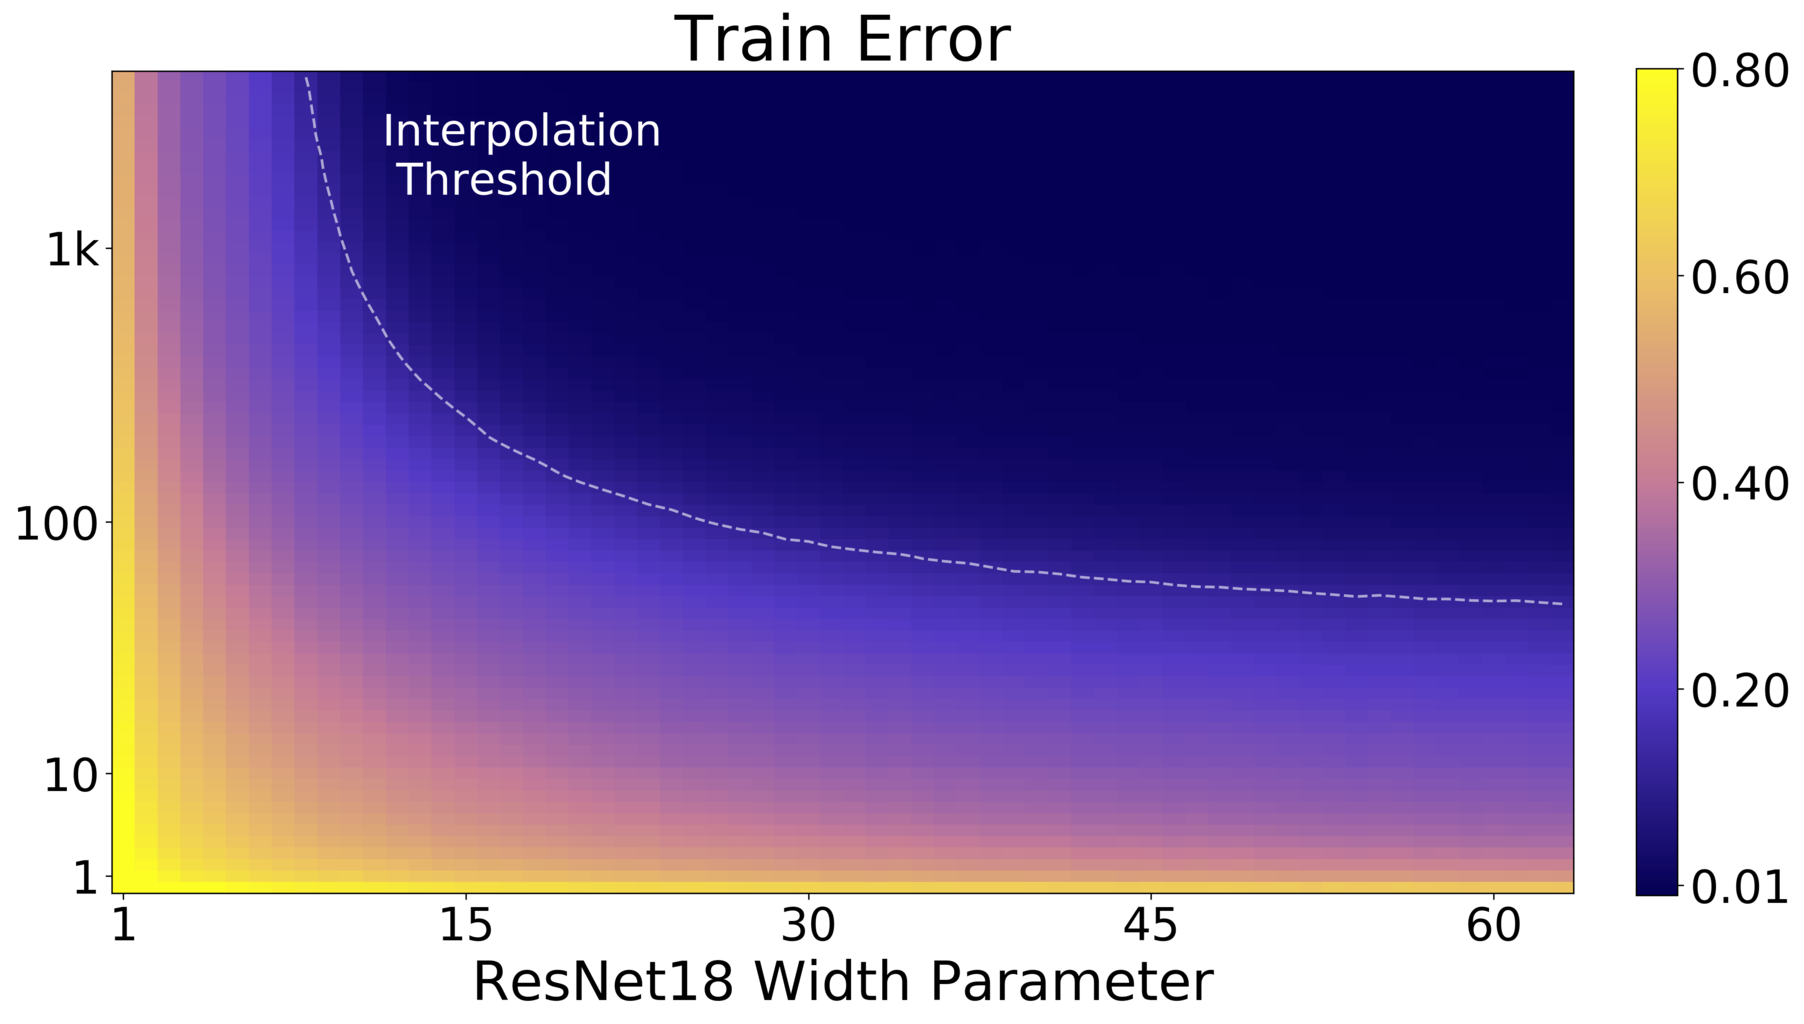
\includegraphics[width=1\textwidth]{media/Rn-cifar10-p15-adam-aug-train.png}
\end{minipage}
\caption{{\bf Left:} Test error as a function of model size and train epochs. The horizontal line corresponds to model-wise double descent--varying model size while training for as long as possible.
The vertical line corresponds to epoch-wise double descent,
with test error undergoing double-descent as train time increases.
{\bf Right} Train error of the corresponding models.
All models are Resnet18s trained on CIFAR-10 with 15\% label noise,
data-augmentation, and Adam for up to 4K epochs. Reused from \cite{nakkiran_deep_2019}}
\label{fig:unified}
\end{figure}

They define \emph{effective model complexity} of $\mathcal{T}$ (w.r.t. distribution $\mathcal D$) to be the maximum number of samples $n$ on which $\mathcal{T}$ achieves on average $\approx 0$ \emph{training error}. This is an entirely empirical definition, similarly per definition as VC-dimension. 

\newcommand{\EMC}{\mathrm{EMC}}
\begin{definition}[Effective Model Complexity]
The \emph{Effective Model Complexity} (EMC) of a training procedure $\cT$, with respect to distribution $\cD$ and parameter $\epsilon>0$,
is defined as:
\begin{align*}
    \EMC_{\cD,\eps}(\cT)
    :=  \max \left\{n ~|~ \E_{S \sim \cD^n}[ \mathrm{Error}_S( \cT( S )  ) ] \leq \eps \right\}
    \end{align*}
    where $\mathrm{Error}_S(M)$ is the mean error of model $M$ on train samples $S$.
\end{definition}

Using this definition, their main hypothesis can then be stated as the following three-fold regions:

\begin{hypothesis}[Generalized Double Descent hypothesis, informal] \label{hyp:informaldd}
For any natural data distribution $\cD$, neural-network-based training procedure $\cT$, and small $\epsilon>0$,
if we consider the task of predicting labels based on  $n$ samples from $\cD$ then:
\begin{description}
    \item[Under-parameterized regime.]  If~$\EMC_{\cD,\epsilon}(\cT)$ is sufficiently smaller than $n$, any perturbation of $\cT$ that increases its effective complexity will decrease the test error.
    \item[Over-parameterized regime.] If $\EMC_{\cD,\epsilon}(\cT)$ is sufficiently larger than $n$,
    any perturbation of $\cT$ that increases its effective complexity will decrease the test error.
    
    \item[Critically parameterized regime.] If $\EMC_{\cD,\epsilon}(\cT) \approx n$, then
    a perturbation of $\cT$ that increases its effective complexity
    might decrease {\bf or increase} the test error.
\end{description}
\end{hypothesis}

It is to notice that this definition is also only observational. By that, it only outlines the specific region of interest where the paradigm shift is identified through experimental results. It has no effective predictive power, or rather descriptive power more than setting up hypothesis with respect to the effective model complexity, and some arbitrary perturbation. \cite{nakkiran_deep_2019} also noticed this difficulty in providing a theoretical definition and theorem regarding such hypothesis, as said in their manuscript. The existence of the critical regime is also not defined. 

The behaviour itself has been particularly investigated, in certain settings. For example, before \cite{belkin_reconciling_2019}, \cite{advani2017highdimensionaldynamicsgeneralizationerror} investigated the generalization error in neural networks of high-dimensional measure. Of such, various behaviours that bear similarity to double descent can be observed. \cite{belkin2018understanddeeplearningneed} expanded on his previous research on the particular subset of kernel learning models, providing a theoretical analysis of specifically the Laplacian kernel on standard neural network. \cite{mei2020generalizationerrorrandomfeatures} investigated random feature regression in such regard, and also found similar results. 

The fact that double descent is not well-defined itself is a problem on its own. Up to the author's knowledge and of myself, there has been no effective definition or given description that outlines specifically how double descent can be structured. Instability in reproducing experiments and the effective range of the phenomena remains a question on its own. 

\section{No-free-lunch}

There is an interesting observation that can be made using the above formalism of the learning theory. From what we can see, if we can guarantee that $\hat{R}(h)\approx R(h)$ by their resolution, then we apparently can generalize the model fairly well, since it is approximately looking at a clear picture of the concept itself. Thereby, the following theorem is guaranteed in such case. 

\begin{theorem}[\cite{10.5555/2371238}]\label{thm:minimalNeu}
    For fixed $\mathcal{H}$, for fixed and sufficiently large $\mathcal{S}$, and no observation errors, the empirical risk is the generalization risk: \begin{equation}
        \underset{\mathcal{S}\sim \mathcal{D}^{m}}{\mathbb{E}}[\hat{R}_{\mathcal{S}}(h)]  = R(h)
    \end{equation} 
\end{theorem}
\begin{proof}
    By linearity of the expectation, and the fact that we assume the sample is given i.i.d., we can write: 
\[
\underset{S \sim \mathcal{D}^m}{\mathbb{E}}[\hat{R}_S(h)] 
= \frac{1}{m} \sum_{i=1}^m 
\underset{S \sim \mathcal{D}^m}{\mathbb{E}} 
\left[ \mathbbm{1}_{h(x_i) \ne c(x_i)} \right] 
= \frac{1}{m} \sum_{i=1}^m 
\underset{S \sim \mathcal{D}^m}{\mathbb{E}} 
\left[ \mathbbm{1}_{h(x) \ne c(x)} \right],
\]
for any \( x \) in sample \( S \). Thus,
\[
\underset{S \sim \mathcal{D}^m}{\mathbb{E}}[\hat{R}_S(h)] 
= \underset{S \sim \mathcal{D}^m}{\mathbb{E}} 
\left[ \mathbbm{1}_{h(x) \ne c(x)} \right] 
= \underset{x \sim \mathcal{D}}{\mathbb{E}} 
\left[ \mathbbm{1}_{h(x) \ne c(x)} \right] 
= R(h).
\]
which yields the desired result. 
\end{proof}

However, this theorem is fairly optimistic. By default, it assumes that the observations provided on $c$, given by the distribution $\mathcal{D}(x)$ represents such mapping $c:X\to Y$ is not fallible, that is, the observation is of $c(x)$ itself. Furthermore, it assumes of a fixed dataset with sufficient size, suggesting only in such case that for $|\mathcal{S}|\to +\infty$ of all discrete, non-overlapping sample size, then $\hat{R}(h)=R(h)$ and hence optimization can be conducted on the exact measure of the general concept itself. This can be considered the \textit{best-case scenario}, in a sense. In reality, this is not always a guarantee. 

When talking about learning capacity of a model, we often think of its ability to perform on certain task class, for example, approximating $c\in \mathcal{C}$ of class $\mathcal{C}$ using class $\mathcal{H}$. Even if we accept the setting of Theorem~\ref{thm:minimalNeu}, there always exist a fundamental theorem called \textit{no-free-lunch} that state that, even of the fixed problem class $\mathcal{C}$ itself, $h\in\mathcal{H}$ can still fail. 

\begin{theorem}[No-Free-Lunch]
    Let $A$ be any learning algorithm for the task of binary classification with respect to the $0-1$ loss over a domain $\mathcal{X}$. Let $m$ be any number smaller than $|\mathcal{X}|/2$, representing the training set size. Then, there exists a distribution $\mathcal{D}$ over $\mathcal{X}\times \{0,1\}$, such that: 
    \begin{enumerate}
        \item There exists a function $f:\mathcal{X}\to \{0,1\}$ with $L_{\mathcal{D}}(f)= 0$. 
        \item With probability of at least $1/7$ over the choice of $S\sim \mathcal{D}^{m}$ we have that $R_{\mathcal{D}}(A(S))\geq 1/8$. 
    \end{enumerate}
\end{theorem}

Of course, this theorem is not perfect, and is often expressed within a weaker version, as seen of its binary expression. Furthermore, it assumes black-box model style, which is typical in machine learning assumption of worst-case learning. Nevertheless, under said assumptions, we can consider perfect learning to be impossible. The NFL theorem for hypothesis classes essentially says that without assumptions about the structure of the target function, no hypothesis class is universally better than any other. It is also considering a hypothesis set of fixed $\mathcal{H}$, with no sustained variation. A disadvantage of this theorem is the fact that it does not take into account of several aspects, for example, the structure and implementation of the hypothesis object itself, the narrow vision of the objective with objective function optimization, and so on. Nevertheless, it implies that no algorithm or hypothesis is superior to other, average over all possible structure. This type of average can be considered simply as either internal average of external average, depends on interpretation of matching $\mathcal{H}\mapsto \mathcal{C}$. That is, superiority in-class and superiority out-of-class that the algorithm is configured of, for example, between $h_{1},h_{2}\in \mathcal{H}$ or $h_{1}\in \mathcal{H}_{1}$ and $h_{2}\in \mathcal{H}_{2}$, for $\mathcal{H}_{1}\not\subset \mathcal{H}_{2}$. The pushback however, then, comes in the form of double descent, is that within the same-class differential, specific version of $h\in\mathcal{H}$ outperforms all the other configuration, of which then happen more than once - which is why we said it is 'double'. 

While it is fairly observable that the bias-variance setting is a special case of NFL - fixed objective function, infinite hypothesis class, we can observe that even within such case, NFL breaks down completely. Thereby, in said case, NFL should not be of concerned with us fairly much. But it raises an important point about analysing the space of structural hypothesis and objective landscape. 

\subsection{Sensitivity of hypothesis}

Some intuition or observation can be made using NFL examples. While it is true that of the subset problem on infinitely many hypotheses and singular objective function class NFL does not hold simply because of double descent and bias-variance tradeoff, it highlights the need for sensitivity analysis of the hypothesis class. Specifically, about the learning setting itself. 

NFL is concerned with the abstract structure of $\mathcal{H}$ and $\mathcal{C}$. In other word, it is not about the model itself, but the communication-in-learning between the two. As such, factors in between can affect how the problem converges and so on, especially with the practical proxy-generalization method of partitioning dataset into testing and training quartile. 

\section{Previous attempts}

Ever since \cite{belkin_reconciling_2019}, despite the general chaotic view of double descent that seems to hold up pretty well, many researches have been conducted throughout, trying to observe or explain it, as we briefly mentioned \cite{nakkiran_deep_2019} as one of such main paper. Before attempting to do anything, and to further contribute with hypotheses forward, we will have to resolve to review previous coursework on such matter. Most of those works include some on theoretical analysis, some on dissection of optimization method then speculation of possible hindsight, some on experiments and observable effects, and so on. 

As such, the first thing to do is to contrive the consensus on `what' constitutes double descent, at least per observable results, by delivering a conjecture. 

\begin{conjecture}
    On the landscape of double descent, model complexity versus generalization error, there exists a fundamental point $\mathcal{M}_{0}$ of model complexity axis, where $dR(h)/d\mathcal{M}< 0$ for $\mathcal{M}> \mathcal{M}_{0}$, which is the interpolation point. 
\end{conjecture}

While this is not perfect, it provides us with a general idea on where to look for double descent. With this, we are ready to follow up the literatures in provision of said questions. 

\subsection{Discovery of double descent}
While double descent is discovered by \cite{belkin_reconciling_2019} and further on modern deep learning landscape of \cite{nakkiran_deep_2019}, it remains that the conclusion is not reached if there exists some fundamental models that would not have double descent, the consistency of double descent through different models entirely and so on. This is mainly because of a particular `shock effect', since before double descent, bias-variance holds the candle as the main principle of choosing and optimizing models to its optimal saddle point. Suddenly by then we observe double descent, which introduces the interpolating threshold $\mathcal{M}_{0}$, that breaks this principle. There is then the open question on how far-reached is double descent in consideration of different architectures, and this is reflected in several papers above. As of now, the main structures that have been verified includes
\begin{itemize}[topsep=1pt, itemsep=1pt]
    \item \textbf{Classical models} \cite{Yang_2024,nakkiran2019moredata,schaeffer_double_2023,lafon_understanding_2024} (linear regression and classical polynomial), \cite{NEURIPS2024_2d43f7a6} (linear regression upon least square), \cite{liu2021kernelregressionhighdimensions}, \cite{zhang2024manipulatingsparsedoubledescent,allerbo2025changingkerneltrainingleads} (kernel methods/regressions), \cite{brellmann2024on} (Classical MSBE-LSTD\footnote{Mean-Squared Bellman Error and Least-Squared Temporal Difference} optimization), \cite{harzli2023doubledescentcurvesneuralnetworks} (Gaussian process). Some papers also have experiments on Random Fourier Feature Networks, and so on, but not substantial (including \cite{belkin_reconciling_2019} paper). 
    \item \textbf{Deep neural networks}: \cite{luo2023doubledescentdiscrepancytask,Yang_2024,pezeshki2021multiscalefeaturelearningdynamics} (CNN, VGG, ResNet, DenseNet), \cite{nakkiran_deep_2019} (Transformer), \cite{shi2024homophilymodulatesdoubledescent} (GNN). 
\end{itemize}

Most of the experiments are concerned of seeing and analysing double descent, basic analysis and experimental observations, test case scenarios for different models and setting and so on. All of the above models are then considered to be, concretely, reported of observing double descent, through various testing scenario on them. Review papers and literatures can be found as \cite{schaeffer_double_2023,ErdongHu2021}, and \cite{shi2024homophilymodulatesdoubledescent} on specifically, graph neural network. 

\subsection{Theoretical attacks}

Because of its intrinsic nature, where double descent breaks the long-standing principle of learning selection, theoretical resolutions has been employed to tackle such problem. Indeed, for example, \cite{cherkassky2024understand} and \cite{lee2022vctheoreticalexplanationdouble} aim toward such direction by understanding the behaviours of double descent using the classical VC-theory approach. However, such papers only introduce, or relate double descent to VC-theory via phenomenological approach - for example, reducing the VC-dimension while fixing or reducing training error, or by examining a potential proxy between the VC-bounds and potential factors encapsulated in the quantities involved. They however, do raise voices of certain inherent problems lies within the theory of learning and in general, learning models. 

Beyond such, certain discovery and inquiries help in having a clearer picture on the behaviour of double descent through various structures. For example, \cite{hastie2019surprises}, under pretext of studying high-dimensional ridgeless ($\ell_{2}$ norm) interpolation, analyse the case of \textit{isotropic features}, \textit{correlated features}, misspecified model (feature observation inhibited), on ridgeless interpolation of linear model, and soon as nonlinear model and latent space model. While strong, their results are restricted to a specific class of assumptions and structure, and is doubtful to be extended further. \cite{allerbo2025changingkerneltrainingleads} investigated and find a particular double descent trace when changing kernel during training, specified in the term of the minimum allowed bandwidth. The kernel bandwidth $\sigma\geq 0$ of a specific kernel filter determines the information smoothing, hence implies the complexity abides by the kernel structure, as well as determine the smoothness of information indicted by the term. 

The sentiments that are shared in between researchers on the topic of double descent vary, but have some common roots, most of them coming from the difficulty to fully assess double descent and its factor components. While double descent concerns the evaluation of \textit{generalization (test) error}, and the \textit{model complexity} notions, the error in question is often implicitly defined or loosely considered in one way or another, and model complexity has no general consensus on its definition. In fact, this points out a very potential, if not already mismatch in the theoretical development. While optimizations and phenomenological aberration of models, as well as building and constructing models at will are well-developed, the definitions on which they are defined on is not fully understood, if not undefined. As of now, literatures on model complexities like \cite{modelcomplex_exp,hu_model_2021,janik2021complexitydeepneuralnetworks,truong2025rademachercomplexitybasedgeneralizationbounds,luo2024investigatingimpactmodelcomplexity} introduce their variations or a copula of different definitions altogether, where some are concerned with its effective complexity, some are concerned with its expressive or structural complexity with different ways to define the model underneath, from parameters to units, to random standard variables (\cite{neal2018modern}). There is also the rift in consideration between classical theory, of which mainly is for classical models, and modern deep neural network structures of which do not conform to such analysis.

\subsection{Problems}
There are a lot of problems regarding how we treat the problem, how we see it, and how we actively analyze it. Most of them lies in the space of statistical learning theory, since bias-variance on itself has variations and justification that is seemingly very natural in statistical theory, like the other version name \textit{approximation-estimation error tradeoff}. All of them contribute somewhat to the current outlook, and so far, it has been pretty bad, than what is being advocated of. Nevertheless, let us state them out, even if missing some particular details. 

\subsubsection*{Problem 1. Authoritative statements}
Despite its prevalence in particular research interest, double descent itself has no definite statement to describe its particular behaviour. This is also true for a list of other phenomena, such as \textit{grokking} (\cite{power2022grokkinggeneralizationoverfittingsmall}), \textit{emergence behaviours} (\cite{wei2022emergentabilitieslargelanguage}, typically discussed in large language models, which is understandable of large-scale specific ruling system), \textit{implicit bias} (\cite{soudry2024implicitbiasgradientdescent}), and \textit{neural scaling law} (\cite{kaplan2020scalinglawsneurallanguage,wei2022emergentabilitieslargelanguage}). There is also \textit{catastrophic forgetting} (\cite{vandeven2024continuallearningcatastrophicforgetting}) which is still fairly native of large systems; nevertheless, those phenomena will be of target later on (or discussed in later chapters). The fact remains that we only \textit{partially understand} these particular results with conjectures and theories to support the facilitation of new insights, new analytical lens, and nothing much. Without a clear definition of what is even double descent, sometimes, we cannot proceed, lest to say even solving it. This is particularly troublesome, since the current theory is so messy and not rigid that many even turns to exotic choices, like topological informatics learning theory, \textit{Homotopy Theoretic and Categorical Models} (\cite{Manin_2024}), and several more. So this is definitely one of the main problem to pushback on. 

\subsubsection*{Problem 2. Model complexity}
The notion of model complexity can be said to be often not so well-defined. There are attempts by \cite{hu2021modelcomplexitydeeplearning,luo2024investigatingimpactmodelcomplexity,barceló2020modelinterpretabilitylenscomputational,Molnar_2020,janik2021complexitydeepneuralnetworks}. The problem of model complexity is not so apparent until the inherent complex nature of models, typically in deep learning models (based on the MLP architecture) is observed to cannot be treated in similar way as classical models. In \cite{hu2021modelcomplexitydeeplearning}, most deep learning models are based on, and investigated of their complexity through measures like the expressive capacity, the effective capacity, and so on; aside from other teams and researchers investigated it by using computational complexity, or functional decomposition. One promising aspect of this is \cite{Molnar_2020}, where we are able to decompose the functional form a specific model into variations of its complexity. 

Nevertheless, it is reasonable to say there are no conclusive measure or definition of a model's complexity. Considering that double descent also appears outside the range of deep learning model, and is somehow consistent in classical models (for example in models tested by \cite{belkin_reconciling_2019}). This is particularly troublesome, as a theoretical analysis requires such definition, especially when the relation of interest is directly involved in such manner. This is a particular aspect needed to be resolved if there are to be progress made in this investigation. Additionally, the concept of overparameterization and underparameterization is also a problem, especially since its definition is not well-defined, hence become a problem in analysis by identifying the classification of the problem setting. 
\subsubsection*{Problem 3. Model structure}

In modern practice, the theoretical and formal treatment, rigorous consideration of different model structures and complexity is not realized. Partially, this is due to the bloom of machine learning and artificial intelligence from the early 2000s. Currently, there has been no conclusive theoretical definition or formulation about the structure of different models, typically can go under the name of mathematical modelling hypothesis, in a way that unify certain properties between architectures. Heuristics are also often employed in several newer models and widely-utilized structures typically seen in large-scale systems, leading to difficulty in formalization and factorization of affectants. 

\subsubsection*{Problem 4. Theoretical insufficiency}

The setting surrounding the learning theory, machine learning models is generally missing of its rigours and analytical properties. Most of the learning setting and model's training-testing setting are often narrowly stated in theoretical sense, and there are a lot of diffusing details that might or might not affect the model's perturbation without knowing. This in a certain way leads to the complexity in analysing different problem setting and experimental results, since the architecture used, the setting considered, model in questions, configuration (either custom or on system side) are not consistent overall. 

Furthermore, a lot of terms, definitions are often hand-waived in papers or in discussions. This also led to the point that in \cite{nakkiran_deep_2019}, they have to somehow 'reinvent' another type of model complexity itself, albeit unsatisfying of a definition, is still a new kind of definition per insufficiently of such. while it is welcome to introduce new definitions, the fact is that it is subjectively inconclusive of terms, definitions and thereof leads to the perception and situation where multiple studies can be found, but all of them are defined on different ground.

Analysing statistical learning theory and overall landscape of statistical learning theory, and the learning theory as a whole, encountering new problems like double descent also revealed its weakness, and ultimately, perhaps one of the reason why it is ineffective against such problem. First, there are simply too many assumptions made, too many formulations made during said process. Furthermore, there are also unclear notions and concepts, of which make it even harder to analyse or fully formalize. Secondly, there are inherent conflicts and uncertainty within those theories, formulations and notions by itself. For example, in one sense, the No-free-lunch theorem is considered to be representative and true, whilst also simultaneously being considered the opposite of such. And amidst abnormality behaviours of the old bias-variance formulation, we also find distinctive weakness in our theory, for example, the concerning difficulty in defining the notion of \textit{model complexity} in various contextual ways. To analyse double descent, perhaps we also need a new theory or formulation to support it. \footnote{Furthermore, most of the general solution and bounds created by statistical learning theory is often in a very simplistic system. For example, if we are to utilize the Rademacher complexity measure (\cite{10.5555/2371238}), most of the time we will have to compute it through the growth function $\Pi_{\mathcal{H}}(m)$ for $m$ points, on the standard finite hypothesis class $\mathcal{H}$ such that 
\begin{equation}
    \Pi_{\mathcal{H}}(m) = \max_{x_1, \dots, x_m \in \mathcal{X}} \left| \left\{ (h(x_1), \dots, h(x_m)) \mid h \in \mathcal{H} \right\} \right|
\end{equation}
Most of our problems resolve to binary classification, or rather, the problem of pattern recognizing discrete, reduced classification form. It is not so sure for now if all problems can be reduced to such way, so we cannot draw conclusive analysis that is not diluted of mathematical formulation for complex systems. That is not to count the computationally intensive operation required to calculate the supposedly classical measure, while not entirely of itself holds any substantial reasonable information about the internal dynamics of the model itself. }

Another problem with classical analytical solution is that it is very \textit{loose}, almost too loose to even considered of such. But sometimes it is too \textit{rigid} in a sense such that it simply does not work at all. Indeed, basing our works and foundational assumptions on top of approximation theory is not quite good at all, because they are very limited. Overall, we can say it is not equipped for handling similar situation. For example, almost all bounds that is subjected of classical learning theory only guarantee particular existential theorem, under very simplified and specific situation without the virtue of extending it to a more general setting. 

This is particular event or rather pattern that we often see in learning theory development, or machine learning theory in general - the `\textbf{mathification}' of a theory. Even though we need mathematics on either end, the approach is impractical or simply wrong, believing mathematics to be the singular thing that defines learning theory. This has many fallacies that can then be attributed to a lot of factors and whatnot, of several factors that plague this analysis even further than just the problem of double descent. For now, 
\begin{enumerate}[itemsep=2pt,topsep=1pt]
    \item Epistemological limits and interpretations (\cite{electronics13020416}) - We ultimately lack understanding of a lot of things. While those `theorems' are very nice in learning theory, the real picture is that it is not real learning, for the word learning are not even defined, as such is to compare them to \textit{human learning} on itself. Even by then, theorems are severely limited. Certain voices also concern of similar problem, including \cite{lipton2016mythos,doshi2017towards,molnar2020general} (\cite{molnar2020general} shortly consider the misleading interpretation question instead), and philosophically, with several pushbacks on structural anecdotes, \cite{dreyfus1965alchemy,dreyfus1972what,dreyfus1986mind,suchman1987plans,brooks1991intelligence,searle1980minds,mccarthy1969philosophical,harnad1990symbol}. On the more modern side, of contemporary critiques, \cite{pearl2009causality,marcus2018deep,sutton2019bitter}. Of the Chinese Room Argument, perhaps we can look into already copulated passages. 
    \item Applying wrongly, and is used to impress and not to explain anything (\cite{lipton2018troublingtrendsmachinelearning}) - mathematics is used to \textit{impress} certain demographic of reviewers and readers, to provide a sense of rigours, to further enhancing the image of formal theory to the point that such theory, even if wrong, can be considered fairly correct by the sheer volume of practitioners believing in such. Such is to say the \textit{mathiness} is turning things into ideology more than rigours itself, of which we can take a tangent to see in economic theory, one of the place to adopt a large portion of machine learning statistics, the pushback against such cursed devolution (\cite{romer2015mathiness,syll2024postreal}). Such can also be seen in generally most double descent analysis, in which there exists many formalisms yet not definite result on double descent. 
    \item Reproducibility and acute false claims (\cite{kapoor2022leakage}) - In general, what we have done cannot be recreated, in certain way, and of certain too optimistic setting that is seemingly unrealistic - particularly in adoption toward practical means of actions. Certain theoretical assumptions and formulations are too stricts, of which means the increment of hypothesis fluctuation with removal of such constraints. 
\end{enumerate}
While most of those are not directly related to our problem - suffice to say the general narrative is so, it particularly indicates a very serious error in the theoretical development itself, and the scope of its reach has been perhaps confirmed at hand. Attempts to solve this problem might need to be an entirely new framework, of something that unify the theory at-hand, or by relinquished attendances to the current dilemma using old and trusted foundation, yet will inevitably fail to resolve further outcome of the solution since its onset is beyond the classical theory. Such is to say, we need an entire solution to cover this particular track. One is promising of them all, being the \textit{Neural Tangent Kernel} (\cite{Jacot:2018:NTK}), but other than that, nothing much came through. 

\subsection{Bounding inequalities}

We briefly mentioned classical learning theory in accordance to our analysis. In particularly, we would like to draw out the fundamental results that have been driving learning theory, and what they say beforehand of the analysis. Would it just only that the old theory being misrepresented, misinterpreted, or there exists some fundamental restriction of the theory that lead to bias-variance being considerate of such setting only, with certain strong assumptions that lies within the theory itself, and can be extended or removed toward generality. Such is to say quite a bold claim, but worth to consider pursuing it. 

In consideration of the PAC-ERM bound, of which restrict $R(h)$ and $\hat{R}(h)$ on some particular restriction, at least for ERM, they are fairly implicit in nature. We will have to reinterpret what they are saying to us, since it does not make much sense usually so. But the general pitfall that we have to be careful of usually lies in the nature of the bounds themselves. Specifically, their fame of being rather existential guarantees but no process-based analytic. 

The first point of approach comes from either the \textit{Probably Approximately Correct} framework and its variation (we would like to talk of the singular original framework) or the \textit{Vapnik-Chervonenkis} framework of learning guarantees. Both of them serve what is there to be called a learning bounds within finite hypothesis class, or by reduced optimization problem with estimators. PAC bounds typically guarantee the upper, worst-case scenario bounds, while VC-dimension of its own definition is typically used for general lower bounds. Nevertheless, we have to know how they work to interpret and use them correctly.

PAC-learning criteria started by specifying a restriction bound in which, the probability that the generalization error can be achieved, for error margin $\epsilon > 0$, is less than a confidence point of $1-\delta$ for $\delta > 0$. How they did this? Well, by bounding the error under specific $m$ samples of the observation space such that the above criteria is guaranteed, given $m\geq poly(1/\epsilon, 1/\delta, n,size(c))$ where $size(c)$ is the representation space of the concept to be learnt from, and $n$ is the input-dimension on itself. Basically, the guarantee under worst-case scenario, whether the generalization error evaluated of the algorithm $\mathcal{A}$ be specifically satisfying the criterion. This, is a \textit{concept-aware} criteria - reflected by specifying the general copula, restricting the algorithm and consider the term of the \textit{ambiance space} \footnote{In general notion, the ambiance space is what we called the \textit{object collection set}, containing the system's dynamical components and what to consider of itself. Basically, the $S$ in the mathematical modelling setting} $\mathbb{A}=(\mathcal{C},\mathbb{I}(n,m))$ upon the evaluator correspondence. The advantage of this method is well-known - it bounds, for example, for how many samples would it be possible to learn, under the assumption that the algorithm $\mathcal{A}$ can indeed, learn such that $h^{*}$ of the final result is $\inf_{h\in\mathcal{H}}\hat{R}(h)$, within polynomial expression of $m$. However, the implication of PAC-learning, is large and fairly difficult to attend to, such is to say they also consider the consistent and inconsistent case already, which is good, but still fairly not so straightforward in particular expression. 

For example, PAC-learning on ERM principle requires that, for some particular notion of the bounding method, such that the following bound will be true, 


\begin{proposition}\label{prop:PAC_ERM_1_recite}
    For any $h\in\mathcal{H}$, for any $\delta\in(0,1)$, 
    \begin{equation}
        \mathbb{P}_{S}\left( R(h) > \hat{R}(h)+ C\sqrt{\frac{\log{(1/\delta)}}{2n}}\right)\leq \delta
    \end{equation}
\end{proposition}

This bound works, under scrutiny assumption such that $c$ and $h$ effectively does not matter in such case, and only use the concentration inequalities on the estimated empirical error on loss function of a particular setting. This is by itself, not so rigorous, and not of the spirit of the PAC-learning boundary itself. The guarantee itself is, controversially, not even a good one. At least for our interest, it does not say anything about the algorithm, or about the hypothesis internal mechanics (if the mechanistic model is exposed, like when the concept class is defined, usually, the hypothesis is supposed to work the same way, which is indeed, not the case). What we miss here, is a lot of those factors together. Nevertheless, the PAC-learning bound indicates a particular insight. We have to \textit{formalize} the instance/observational space; we will have to formalize, of it, the sample $m$, the dimension of the encoding $n$, the representation system used by $size(c)$, the concept, and indeed, of the structure of the hypothesis space $\mathcal{H}$ of which gives detail to the hypothesis itself. Such is to say, we need to somehow make the PAC-criteria to be \textit{structural-aware}, per meaning of the word. 

For VC-theory and the concept of its dimension, its limit is again, well-known up to certain accordance. Classical VC-theory worked upon a fairly restricted, discrete framework of classification, usually binary classification (for SVM) for example, on \textit{shatterable concept space}. The more, fairly advanced version of \textit{fat-shattering} and multiclass-VC domain still fall short of the generality and more complex structure - in which case we mean the simpler the restriction on what the task is. Insights and ideas toward VC-theory is rather explicit of its own principle - fundamentally speaking, VC-theory conjure to the \textit{combinatorial VC-dimension} of all possible solvable system, up to certain data points, of certain class, except of special cases. Such is to say that one of the aspect that Vapnik-Chervonenkis theory focus on is one particular \textit{expressive complexity} of a specific model. This is also a problem that we have to solve. 

Classical Rademacher is also very hard to justify of its use here. Classical Rademacher analysis typically refers to the application of \textit{Rademacher complexity}, a near-empirical theoretical definition of complexity class. One advantage that it poses, against VC and PAC-based structures, is that the ambiance space of Rademacher complexity is not restricted toward particular class of problem, like binary labelling of the other theoretical analysis. Nevertheless, Rademacher complexity is unstable (leading to its dilemma of having very few closed-form results) and computationally difficult. Its bounds are also of the same fate, lest to say some of the results proceeded of the Rademacher complexity are often refuted in empirical experiments. Furthermore, strong assumptions and restricted bound cases still hinders its usefulness. Moreover, it does not have anything reasonable analysis for complex structure other than the plain estimators, especially with structures that exhibit the supposed inductive bias. 

Those critiques against classical analysis is not alone of us. Rather, there are indeed a lot of invoices on such matter toward new development of learning theory. Specifically so, \cite{zhang2017understandingdeeplearningrequires} inquired of the fact that bounds are often vacuous in terms of deriving for deep neural network. Of the same paper is also the opinion that expressivity is not generalization, which is, obviously true from our theoretical preliminary. \cite{truong2025rademachercomplexitybasedgeneralizationbounds} discussed the instability and hard computation of the Rademacher bound, also of threshold behaviours. On the core topic of generalization (which a lot of people pursue for obvious reason), \cite{nagarajan2021uniformconvergenceunableexplain} argued against the current uniform convergence theory that seemingly fail to garner an understanding of such behaviour, and so is \cite{tunali2019empirical}. Solutions exist, yes, but either in the form of partial solution and variation of classical theory, like PAC-Bayes, some way of experimenting, like \textit{stability-based analysis}, \textit{margin/norm measures} or localized Rademacher complexity, as seen in \cite{bartlett2005local,bartlett2017spectrally,bousquet2002stability,neyshabur2015norm}. Nevertheless, they are still \textit{partial solutions}, and no full solution has emerged, yet. We would likely want ourselves to not follow the same path again. 

\subsection{Complexity notions}
Even though such can be said of the pitfall of current practices, it is still not the end of the road, or at least of the principle in which we apply to our empirical study - to force double descent out. Which is rather harder than what it looks like. We might as well attempt to analyse double descent in terms of classical, non-novel theory first, before jumping straight into conclusion without personal observations. First, the issue of bias-variance and double descent is related to multiple factors, but specifically between the notion of bias-variance and complexity-accuracy. However, their definition and usage in certain contexts are obscured, thus would require a fairly thorough consideration. Most of these results contains of bounds and often discussion of random processes, and also restricted itself to mathematically well-defined setting. For now, we would like to investigate their notions and applications. Though for starter, we have to discuss the following preliminary. The hypothesis class $\mathcal{H}$ has two types of classification: either infinite hypothesis class $\mathcal{H}^{\infty}$ or finite hypothesis class $\mathcal{H}^{n}$. Based on the details of the expression of representation strings (\cite{10.5555/200548}), an infinite hypothesis class contains infinitely many specifiers of the hypothesis structure. Note that this does not correlate to an increase in parameter, as we will see with the case of axis-aligned rectangle - for only four parameters $(l_{1},l_{2},h_{1},h_2)$ we can specify all axis-aligned rectangles with their value taken from the field $\mathbb{F}=\mathbb{R}$. Finite hypothesis class is then can be understood of the number of configuration, or in discrete form combinatorial pairs that can be presented of the hypothesis class, for example, a string of all $n$-length binary numbers $\{x_{1},\dots,x_{n}\}, x_{i}\in \{0,1\}$. A subtlety that would then have to discover, is the increment in size of the hypothesis to accommodate either finite or infinite number of specifying parameters - one example can be sampled from is the class of all support vector machine (SVM, \cite{Vapnik1999-VAPTNO}), which for now we treat it as it is. The concept class can then also be treated similarly. Here, we assume a setting where unless specified, we have knowledge of the concept class structures, but not the hypothesis. 

Assume the working space is the real field $\mathbb{R}^{n}$. Let us recall a model $h\in\mathcal{H}$ of certain hypothesis class $\mathcal{H}$. Then, the \textbf{complexity} refers to the complexity of the hypothesis $h$ itself; there is also the notion of class maximal complexity for $\mathcal{H}$. Complexity in this case refers to the mass of the model, or rather, to answer the following questions:
\begin{enumerate}[itemsep=0.5pt,topsep=0.5pt]
    \item What is the effective expression range of a hypothesis?
    \item What is the hypothesis structured in?
    \item If the model is constructed by parameters, how many parameters are there?
    \item How many components are there in specific model $h$, and how would another model $h'\in \mathcal{H}$ differs from $h$?
\end{enumerate}
Those questions are not so easily answered. Specifically, analysis often puts the hypothesis class $\mathcal{H}$ as a class of functions. So, there exists the class $\mathcal{H}_{n}$ of $n$-th degree polynomials, or else. Effective complexity in such case means the range of expression a function can give - for example, for $n$-th polynomial class, we already have the Weierstrass's theorem that tells us that any continuous function of closed interval can be approximated by a polynomial of arbitrary order. These expressions depend on the field or space the hypothesis class lives in, for example, if the hypothesis is configured to work in the set of all functions in $\mathbb{F}=\mathbb{R}$ of algebraic field, then we call it the algebraic family. There are various hypothesis classes in such case, and usually, not a lot of them can be analysed and represented in the same way, and hence also the analysis of the `size' of the hypothesis, also between different hypothesis classes. This prompted the usage of a more general notion, called \textbf{representation complexity}. Representation complexity refers to the number of components needed to express $h$ and generally, any hypothesis in $\mathcal{H}$. This is often the parameters count, since the parameters themselves are used in constructing the function in algebraic system. Thus, again, an $n$-th degree polynomial might have $2(n+1)$ parameters, for $n+1$ variational input (or variable), and $n+1$ coefficients. Notice that we specifically at the beginning, use the notion of algebraic structure $\mathbb{R}$ because of it. If we restrict ourselves to the expression, for example, for $\mathbb{B}=\{0,1\}$, then it can be expressed in various ways in logic theory, such as conjunctive normal form (CNF), disjunctive normal form (DNF), and else. This forbid the analysis based on the effective process itself, but rather the number of components required, hence taking them as complexity of construction. 

Furthermore, the above two measures only talk about the \textbf{general mass} (representation) and \textbf{general expression}. In a deeper analysis, we haven't talked about the general individual complexity of the model itself. This notion refers to the complexity computed or evaluated, by considering the process-dependent behaviours and range of a specific expression influence on the operational process itself. While expressive complexity can provide a sufficient bound of approximation strength, the individual strength that can make it happen (for example, the fact that $n^{k}$ value range versus $n^{k-1}$ value range is totally different by one power degree), the contribution and sum of individual components can only be discussed using the general individual complexity, by using \textbf{process complexity} term. Up until now, this has not been formulated as author's knowledge, hence the two standard term would then be used instead in the analysis. 

\begin{table}[htb]
  \centering
  \footnotesize
  \begin{threeparttable}
    \caption{Descriptions of complexity measures applied to models and learning processes}
    \label{tab:complexity-measures}
    % three columns: adaptive widths
    \begin{tabularx}{\textwidth}{@{} >{\RaggedRight\arraybackslash}X
                                     >{\RaggedRight\arraybackslash}X
                                     >{\RaggedRight\arraybackslash}X @{}}
      \toprule
      \textbf{Measure} & \textbf{Purpose} & \textbf{Remarks / Scope} \\
      \midrule
      Representation complexity
        & Complexity of encoding a model (size of representation, alphabet-dependent).
        & Model-level measure; depends on chosen encoding/representation and can be used to quantify storage or description length. \\
      \addlinespace[2pt]
      Expressive complexity
        & Complexity of the model's observable behaviour (operational expressivity of the mapping it implements).
        & Model-level; measures the variety of input–output behaviors the model can implement. \\
      \addlinespace[2pt]
      Structural complexity
        & Complexity of the model's internal architecture (how components compose and interact).
        & Decomposable into component-wise measures (e.g., per-layer, per-module) and useful for architectural comparisons. \\
      \addlinespace[2pt]
      Structural mass
        & Aggregate representation size derived from representation complexity across the model.
        & Global model measure for total encoded size (e.g., total parameter encoding length). \\
      \addlinespace[2pt]
      Sample complexity
        & Number of samples required to reach a prescribed performance level (statistical sample-count).
        & Process-level measure; depends on hypothesis class, loss, and desired error/confidence. \\
      \addlinespace[2pt]
      Sample space complexity
        & Intrinsic complexity of the data distribution / sample domain (richness, diversity, structured-ness).
        & Statistical measure over the sample space; affects learnability and effective sample size. \\
      \addlinespace[2pt]
      Optimization complexity
        & Complexity of the learning algorithm (convergence rate, computational/iteration cost, sensitivity).
        & Process-level; hard to pin down analytically, often characterized empirically or by worst-case bounds. \\
      \bottomrule
    \end{tabularx}

    \begin{tablenotes}
      \footnotesize
      \item[] \textbf{Notes:} The notion of structural mass is convoluted. In certain setting, it is simply the parameter space $\theta\in\Theta$, but in some setting, there exists fundamental difference than identically weighted parameter space complexity, as seen in multi-basis polynomial models, not taking into account homogeneous deep learning networks. Optimization complexity coincides with PAC-learning bounds for polynomial runtime, and \textit{sample complexity} sometimes can only be the dimension of the input/observation space.
    \end{tablenotes}
  \end{threeparttable}
\end{table}

The above complexity, aside from sample space-related measure, can also be applied onto the concept class's members itself. We also take the class complexity in such case, as the argument that maximize those measure: that is, the largest value of the measure, taken on the class as the class's complexity. 

The next complexity measures that can be taken of, comes from the learning process structure itself. Usually, in statistical learning theory (\cite{STL_Hajek_Maxim_2021,10.5555/2371238,10.5555/2621980}), we often use the setting that is related to \textbf{supervised process}. This usually means the process can be configured in a feedback loop, or induced response toward the model - often come from the observational space, where the concept that is set to be the target of the process - then called as learning process - is conjured. For now, we reserve this to the classical learning theory and process, and will not inquire further of such direction. 

The learning process assumes an operational space containing the structure, for example, $\mathbb{R}$-encoding space of real values, and a set of \textbf{samples} living in such space, denoted $\mathcal{S}$. Those samples are often referred to as the \textbf{observation set} of a particular objective of learning. As mentioned above, $\mathcal{S}$ belongs to the concept $c$, assumed to be of certain concept class $\mathcal{C}$. $\mathcal{S}$ is obtained by using an observing process to create or generate the result. This process can be determined or considered in multiple way, however, generally can be considered by having a deterministic interpretation (using an explicit function $c(x)$) or by probabilistic approach (modelling a distribution $\mathcal{D}$). Hence, we gain another type of complexity, with regard to the process called \textbf{sample complexity} - usually defined of cardinality - the amount of sample needed for particular purpose, for particular objective. For the complexity category up to the structure of the learning setting by itself, we call it the \textbf{sample space complexity}. 

One final complexity that is worth mentioning is then the \textbf{optimization complexity}, measure on the action of the learning algorithm. By such, it investigates the construction of an optimization algorithm solely dependent on its size of the algorithm, and other non-process related measures. Optimization complexity can also be related or expressed, in situation of time complexity, which is typical in computing system. 

One might ask why we need to determine and categorize complexity measures and the need to generalize and differentiate of each one. Indeed, while in usual use cases, such complexity notion can be considered sufficient in controlling and gauging the model itself. However, just as \cite{James2021} indicated in the section on deep learning double descent, such complexity might eventually, of some regions, inadequate to express and evaluate the complexity of the model in its operations anymore. Such transition is unanswered, and while the founding of complexity notion is still fragmented, it is indeed difficult to not paying attention specifically to those notions themselves. 

\subsubsection{Representation complexity}

Representation complexity works in assumption of the wider concept class $c\in \mathcal{C}$. However, it can also be applied onto the hypothesis class $\mathcal{H}$. To define it however, we need to define the concept of a representation scheme (\cite{10.5555/200548}). 

\begin{definition}[Representation scheme]
    For a given concept class $\mathcal{C}$, a \textbf{representation scheme} for such concept class is a function $\mathcal{R}: \Sigma^{*}\to \mathcal{C}$, where $\Sigma$ is the finite alphabet of symbols. We call any configuration $\sigma \in \Sigma^{*}$ such that $\mathcal{R}(\sigma)=c$ a \textbf{representation} of $c$, under $\mathcal{R}$. For any given $c$, the representation scheme might not be unique. \footnote{Perhaps representation scheme can be further realized by applying a Borel $\sigma$-algebra on top, and put on it a perspective measure to handle the notion of representation size. For example, in the traditional example of axis-aligned rectangle, one such representation scheme could be the real number schema $\mathcal{R}:(\Sigma \cup \mathbb{R})^{*}\to \mathcal{C}$, which then can utilize the extended notion of a Lebesgue measure over $\mathbb{R}$ and its spaces.}
\end{definition} 

The representation of a specific concept or hypothesis classes can be different. Consider the learning problem of a Boolean string. The representation can take form as the \textbf{conjunctive normal form} (CNF) or \textbf{disjunctive normal form} (DNF), with their expressiveness on equal, however string length varies exponentially, as seen by \cite{Wegener1987,MiltersenRadhakrishnanWegener2005,DarwicheMarquis2002}. Since the learning algorithm has access only to the input-output behaviour of $c$, in the worst case, it must assume that the simplest possible mechanism is generating this behaviour. Within this assumption, we can now formulate the \textbf{representation size} or \textbf{representation complexity} of particular concept, denoted $size(c)$. 
\begin{definition}[Representation complexity]
    Given a concept $c\in\mathcal{C}$, the \textbf{representation complexity} of $c$ is defined to be the size of the smallest representation of the concept $c$ in the underlying representation scheme $\mathcal{R}$, that is, 
    \begin{equation*}
    size(c) = \min_{\mathcal{R}(\sigma)=c}\{size(\sigma)\}
\end{equation*}
for any string $\sigma$ of the representation scheme $\mathcal{R}$ that still represents $c$.
\end{definition}
Under such definition, the more "complex" the concept $c$ is with the respective chosen representation scheme, the larger $size(c)$ is. This is also where the concept of the concept class $\mathcal{C}$ comes from - it comes from the \textit{representation class indiction} that we have in mind some fixed concept classes we study by their representation scheme. We note that, however, the definition works within the least-lower bound limit - we choose the infimum. In the worst-case scenario, the representation potential mismatch between $h$ and $c$ might be very large, hence the \textit{effective representation} might not be the same. We also operate on the assumption that different representations are equal, even though practically, we do not have the exact form of $c$ to be sure that problems can reduce from one representation to a smaller one - which forms the basis of the \textbf{manifold hypothesis}\footnote{The \textbf{manifold hypothesis} can be loosely expressed in the following statement by Lawrence Cayton \begin{quote}
  [\dots] the dimensionality of many data sets is only artificially high; though each data point consists of perhaps thousands of features, it may be described as a function of only a few underlying parameters. That is, the data points are actually samples from a low-dimensional manifold that is embedded in a high-dimensional space. 
\end{quote}}. Hence, the following assumptions are needed. 

\begin{assumption}
    For every concept $c\in\mathcal{C}$, there exists the representation family $\{\mathcal{R}\}$ of all representation with characteristic shared by each concept $c$. For each $c$, there exists one or more representation $\mathcal{R}$ such that its representation complexity can be defined. A weaker assumption assumes that for $c$ of one or more representation scheme, the more complex representation scheme can always be reduced to a lower representation scheme of minimal complexity.
\end{assumption}

\subsubsection{Optimization complexity}

Optimization complexity refers to the runtime in solving the learning problem by itself. Taken for example, between polynomial and linear regression analytical-probable solution solving time, the complexity lies around $\mathcal{O}(np^{2}+p^{3})$ for the structural complexity defined by $p=d+1$ parameter count (including bias) via ordinary least square (OLS). However, this measure itself is not enough, and is not relevant to our problem, partially because of its operational level usage in runtime, which is often attributed to the learning algorithm convergence bound itself. 

Still, we should give our own idea of such optimization complexity, called simply the $\epsilon$-optimization complexity, rephrased from famous variations already established in the theory of optimization (hence, not a novel definition). 

\subsubsection{Sample complexity}

The sample complexity can be defined in a fairly simple manner. Per usual, sample complexity, in context of learning systems, is defined as the number of training samples that it needs in order to successfully learn a target function. Certain definitions can be found, in for example, \cite{huang2025samplecomplexityrepresentationability,wegel2025samplecomplexitysemisupervisedmultiobjective,Mei2022TowardsBridging} or in a more specific context of active online learning, \cite{Balcan2010TrueSampleComplexity}.  However, such definition is usually too simplistic of the sample complexity itself, or compressed any reasonable information or properties are there of the sample set. Nevertheless, we should still recall the copulated definition, 
\begin{definition}[Sample complexity]
  A measure $\mathcal{M}_{S}$ gauges the \textit{sample complexity} of a learning setting on sample set $S$, if, the learning algorithm $\mathcal{A}(h,c)$ can guarantee, for $M_{S}:\mathcal{P}(S)\to\mathbb{N}$, such that $M_{S}$ outputs a particular value such that for $S_{i}$ the $i$th ordered power subset of $S$, then
  \begin{equation}
    \mathbb{P}_{S_{i}} \left[\hat{R}(h)\leq \epsilon\right] \geq 1 - \delta
  \end{equation}
  If, it can guarantee instead, such that, 
  \begin{equation}
    \mathbb{P}_{S_{i}} \left[\lvert \hat{R}(h) - R(h) \rvert\leq \epsilon\right] \geq 1 - \delta
  \end{equation}
  We call it the \textit{generalization sample complexity} on empirical data. 
\end{definition}
Again, we emphasize the usage of this sample complexity term, however, either we \textit{decompose it} (which is not possible), or we will need to define another notion for \textit{sample complexity} of a given learning setting entirely. Furthermore, statistical metric of the sample set should also be considered. For example, a \textit{statistical-aware sample complexity} can be defined by the $(\epsilon,\mu)$-sample complexity measure on Gaussian spread distribution, as followed. 
\begin{definition}[$(\epsilon,\mu)$-sample complexity]
  A measure $\mathcal{M}_{S}[\epsilon,\mu](h,c)$ gauges the \textit{sample complexity} of a learning setting on sample set $S$, if, for the sample distribution on particular $\epsilon,\mu$, of a random permutation process, the learning algorithm $\mathcal{A}(h,c)$ can guarantee, for $M_{S}:\mathcal{P}(S)\to\mathbb{N}$, such that $M_{S}$ outputs a particular value such that for $S_{i}$ the $i$th \textit{permuted power subset} of $S$, then
  \begin{equation}
    \mathbb{P}_{S_{i}} \left[\hat{R}(h)\leq \epsilon\right] \geq 1 - \delta
  \end{equation}
\end{definition}

This definition sought to connect, in a sense, partially, the statistical analysis of the sample space to the complexity term with respect to the hypothesis $h$. Even though we use the statistical set $(\epsilon,\mu)$ of normal distribution process, a different set can be used, and hence changing the definition accordingly. 

\subsubsection{Structural mass}




\subsection{Classical insight}

Classically, we can see that the problem of double descent is not inherently a problem that can be explained only by considering model complexity and the error rate. As such, it requires a framework that consider multiple factors together, and interpreting different hypothesis. Nevertheless, classical theory does indeed point to certain factors or aspect that should be of concern. For example, we have seen plenty of analysis that indicates that \textit{sample complexity} might be the biggest factor, considering the behaviour is intrinsically operable and perhaps observable in almost any model, except for certain model that is specialized of the data structure itself. Even by then, the error still can be obtained given large enough model disparity to the concept class. There are attempts to, indeed, analyze double descent from a VC perspective (\cite{lee2022vctheoreticalexplanationdouble}), however, the paper falls into the same pitfall as others in their interpretation and analysis. 

Nevertheless, even though we have said plenty of the disadvantage of the classical theory in terms of statistical learning, their insight is valuable in determining the possibility of dynamic in question. 

\subsubsection{PAC-learning setup}

The PAC-learning process (\cite{10.5555/2621980,10.5555/2371238,STL_Hajek_Maxim_2021}) connects three complexity measure - the sample space complexity, representation complexity, and optimization complexity, to the evaluation of the statistical learning process. It refers to the categorization of various learning procedure that satisfies the Probably Approximately Correct criteria in its name, as such being followed. 

We assume no structure of $h$ and $c$. They can be functions, partial functions, relations, complex algorithms, or others. In a typically learning setting, we also have the argument of \textit{preliminary knowledge}, presented in literatures of the term \textit{inductive bias}. For example, if the concept class $\mathcal{C}$ is assumed, then we say the setting is \textbf{model-specific}. If there exists no hard assumption on $\mathcal{C}$, then the learning setting is said to be \textbf{model-free}. Then, the PAC-learning set for model-specific setting is defined as followed. 

\begin{definition}[PAC-learning]
    A concept class $\mathcal{C}$ is said to be \textbf{PAC-learnable} if there exists an algorithm $\mathcal{A}$ and a polynomial function $poly(\cdot,\cdot,\cdot,\cdot)$ of 4-argument such that for any $\epsilon>0$, $\delta>0$, for all distribution $\mathcal{D}$ on $\mathcal{X}$ and for any target concept $c\in\mathcal{C}$, the following holds for any sample size $m\geq poly(1/\epsilon,1/\delta,n,size(c))$: $$\underset{S\sim \mathcal{D}^{m}}{\mathrm{Pr}}\left[ R(h(S))\leq \epsilon \right]\geq 1-\delta$$
    for a given error measure $R(h_{S})$. If $\mathcal{A}$ further runs in $poly(1/\epsilon,1/\delta,n,size(c))$, then $\mathcal{C}$ is said to be \textit{efficiently PAC-learnable}. When such algorithm exists, we call $\mathcal{A}$ a PAC-learning algorithm. 
\end{definition}
This can be easily extended into the model-free case, and further on, which is left in the appendix section. The reason for the argument $size(c)$ is as followed. Consider a class of concepts defined by the satisfying assignments of certain formulae. A concept from this class that satisfies such formulae, can be represented by a formula $f$, a truth table, or any given formulae that is tautologically equivalent formulae $f'$ to $f$. PAC-learning bound argues in the sense of \textit{computational complexities}, and \textit{space complexities}. Specifically, the term $poly(1/\epsilon,1/\delta,n,size(c))$ hopes to bound the required learning process to polynomial time, specified by 4 parameters. Here, $n$ is the \textit{input dimension}, $size(c)$ is the encoding complexity of the target concept, $\epsilon>0$ is the \textit{accuracy bound}, and $\delta$ is the confidence bound - the probability that $h$ fails.

PAC-learning procedure gives, by assumption of a \textbf{consistent learner}, two different generalization bounds for two different cases. We first define the notion of a consistent learning algorithm, or consistent learner, for a concept class $C$ and hypothesis $h$. 
{
    \small
    \begin{definition}[Consistent Learner]
    We say that an algorithm is a consistent learner for a concept class $C$ using hypothesis class $\mathcal{H}$, if for all $n$, for all $c\in C_n$ and for all $m$, given 
    \begin{equation*}
        S = \{ (x_1, c(x_1)) , (x_2, c(x_2)) ,\dots, (x_m, c(x_m))  \} 
    \end{equation*}
    as input, $x_i \in X_n$ outputs, then the algorithm $L$ outputs a hypothesis $h\in \mathcal{H}_n$ such that $$h(x_i) = c(x_i) , i = 1,\dots,m$$ 
    \end{definition}
}
A consistent hypothesis is the hypothesis that is consistent with all the training data provided to it from the concept $c$. The two bounds then contain the debate between consistent hypothesis (i.e., for example, admitting no error on training data, almost perfect - maybe even so), and inconsistent hypothesis, of which have general defects from the actual concept, or even different by a margin. This equates to observational noise $\sigma$, typically used in simulation of noisy feature and spread, and also for randomization. Inconsistent then means the further this particular noise is increase, the higher the lower bound of the error can be for any particular measure, in comparison to the true concept $c$ in consistent case. 

PAC-learning famously leaves two results on the learning bound of the learning setup. 
\begin{theorem}[Learning bound - finite $\mathcal{H}$, consistent case]\label{thm:PAC_consistent}
    Let $H$ be a finite set of functions mapping from $\mathcal{X}\to \mathcal{Y}$. Let $\mathcal{A}$ be an algorithm that for any target concept $c\in H$ and i.i.d. samples $S$ returns a consistent hypothesis $H_{S}$, such that $\hat{R}(h_{S}) = 0$. Then for any  $\epsilon,\delta>0$, the inequality $\mathrm{Pr}_{S\sim D^{m}}[R(h_{S})\leq \epsilon]\geq 1-\delta$ holds if $$m\geq \frac{1}{\epsilon}\left( \log{\lvert H \rvert }+\log{\frac{1}{\delta}} \right)$$
This sample complexity result admits the following equivalent statement as a generation bound: for any $\epsilon,\delta>0$, with probability at least $1-\delta$, 

\begin{equation}
    R(h_S) \leq \frac{1}{m} \left( \log{|\mathcal{H}|} + \log{\frac{1}{\delta}} \right)
\end{equation}
\end{theorem}
\begin{proof}
    See \cite{10.5555/2371238} for the original proof.
\end{proof}

\begin{figure}[htb]
    \centering
    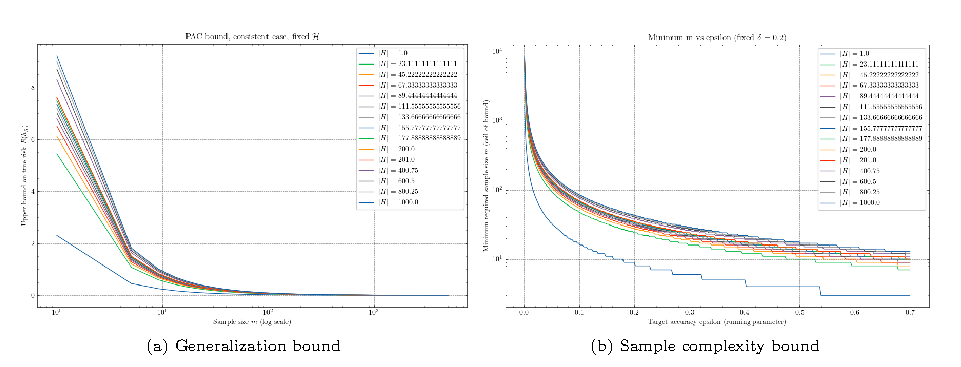
\includegraphics[width=\textwidth]{pdf/PAC_consistent.pdf}
    \caption{The learning bound, both generalization bound $R(h_{S})$ and the sample complexity bound $m$, from theorem~\ref{thm:PAC_consistent}}
\end{figure}

\begin{theorem}[Learning bound - finite $\mathcal{H}$, inconsistent case]\label{thm:theorem_inconsistent}
    Let $\mathcal{H}$ be a finite hypothesis set. Then, for any $\delta > 0$, with probability at least $1-\delta$, the following inequality holds: 
    \begin{equation}
        \forall h \in \mathcal{H}, \quad R(h) \leq \hat{R}_S (h) + \sqrt{\frac{\log{|\mathcal{H}|}+ \log{2/\delta}}{2m}}
    \end{equation}
\end{theorem}
\begin{proof}
    Appendix section.
\end{proof}


For a looser bound, we can ultimately use an $\epsilon$-consistent learner criteria in such case. PAC-learning setting raises some peculiar insight toward the problem itself. First, is the learning bound itself of which raises the importance of several factors --- the dataset size, $m$, of which is used as the \textbf{total resources required} for approximating such function. Furthermore, the set complexity $\mathcal{H}$ is also used, albeit questionably inconsistent in the term $\log{|\mathcal{H}|}$, which implies at least consideration on the cardinality of the hypothesis class. In a finite domain, we notice that PAC-learning of consistent case is exactly the case of interpolation, assuming non-smooth and noisy data, and the inconsistent case describe the wider range of approximation-based case, but does not consider an approximation-aware bound. The design of $|\mathcal{H}|$ also does not allow for certain exact hypothesis class size measurement, except for combinatorial case where $\mathcal{H}$ is indeed finite. Nevertheless, the bound indeed indicates that for $m$ increase, the hypothesis class often do much better in general. 

\subsection{VC-theory}



\clearpage

\subsection{Hypothesis}

In learning and researching of the progress and treatment of double descent, several hypotheses, most of the time observations and insights such, is formed. Hence, there are several hypotheses for what to look out for, as well as the formulation needed to interpret certain phenomena and observations. This ranges from topics of re-evaluating the statistical learning theory, estimation and refactor of assumptions (or \textit{inductive bias} when designing models), to different interpretations and representations that can better explain, model, or gives certain insights.  
\subsubsection{Stability of bias-variance measure}
Stability of bias-variance measure is questionable, as it is in literature (\cite{domingos_unifeid_2000}), loosely defined by defining a 3-dimensional vector $\lambda=(\lambda_{1},\lambda_{2},\lambda_{3})$ for such: 
\noindent 
\begin{equation*}
        \begin{split}
            \mathbb{E}_{\mathcal{D}} \left[d((f,\mathbb{E}[y\mid x])\right] & = \lambda_{1} \mathrm{Bias}(f,y) + \lambda_{2}\mathrm{Var}(f,y)+ \lambda_{3}\epsilon(\mathcal{D})\\ 
            & = \lambda_{1}\underbrace{\left\{ \mathbb{E}_{\mathcal{D}}[f(x;\mathcal{D})] , \mathbb{E}[y\mid x] \right\}}_{\text{bias term}} +\lambda_{2} \underbrace{\mathbb{E}_{\mathcal{D}} \left\{(f(x;\mathcal{D}), \mathbb{E}_{\mathcal{D}}[f(x;\mathcal{D})])\right\}}_{\text{variance term}} +\underbrace{\lambda_{3}\epsilon}_{\text{irreducible error}}
        \end{split}
\end{equation*}
where $\epsilon(\mathcal{D})$ is the irreducible error of the system, depends (theoretically) on the intrinsic imperfection of the dataset $\mathcal{D}$. Assessment on stability of such decomposition is recommended. 
\subsubsection{Alternative measures}
We believe that the bias-variance decomposition is a poor estimation and measure for controlling, validating and choosing model from, at least from the perspective of analysing missing details. Specifically, bias and variance term, as well as their supposed expression of decomposition in the standard loss measure of model effectiveness is not representative, nor expressive of the actual, underlying notion of \textit{model complexity} $C(f)$ and its effectiveness. Furthermore, bias-variance decomposition is not straight-forward of others type of loss functions, except only for some classes of loss function (loss on Bregman divergences and exponential class). This sentiment is shared in \cite{brown2024biasvariance}.

\subsubsection{Inductive bias}
Inductive bias obviously plays a role, as mentioned by some literature \footnote{Most notably, \cite{lafon_understanding_2024}, of which raised particular point about the need of learning with inductive bias as a structural presumption. Additionally, the paper also includes an analysis on the inductive bias of gradient descent, though solutions and particular application on double descent explanation is doubtful.}, though we don't know exactly how the inductive bias can be formed to play any role in the central dynamic of the model operating process. Certain assumption, for example, the \textit{convexity of the loss function} might actually affect the model as it is, and introduce unwanted patterns in the following process. 
\subsubsection{Randomness and probabilistic setting}
Random initialization of parameters, as well as the initial conditions of the model initialization process might also be taken into account. Obviously, this is not a new insight, and is rather a very old one, however, this approach still has varied potential for interpreting double descent. Scaling up/down this effect might result in new insight, as well as inspecting the uncertainty and diffusion patterns in large-scale model deployment, in which from an end-to-end perspective requires several space transformation operations in successions.
\subsubsection{Knowledge masking}
The very ambiguous idea or treatment of statistical learning, as well as machine learning, is the idea of masked. Or, paraphrased, \textit{hidden information} regarding the underlying process of estimation. Specifically, for example, we tend to assume things to not be able to grasp - either the probability $p_{X}(c)$ of the concept class, the distribution $\mathcal{D}$ specified to such input distribution, or the concept class $\mathcal{C}$, Markov properties, etc. We would like to formalize this notion as soon and as such in the most direct way, as it is one source of the many assumptions that we have in concession of theoretical results. 
\subsubsection{Intrinsic Data Factors}

The effect that data has on the model should also be taken into account, as of fact. As far as we are concerned of, the shape, practical system that the dataset gives the setting, the factors running into the dataset, the choice of the dataset being sampled, selected in partitions, and other factors must also be analysed. Without such, we leave `gaps' in which sensitive, potentially chaotic behaviours might occur frequently and would not be identified, or being classified into irreducible errors, static of the learning setting. As such, we might as well list a few potential points of interest. 
\begin{enumerate}[itemsep=1pt,topsep=0.5pt]
  \item \textbf{Data distribution}: the distribution of the dataset itself affects how the concept is represented in the space. If the representation space created by using the data is large, but sparse, then the condition would make for some behaviours to occur more easily. This is one degree of freedom of the system setting. If the dataset spread is low, yet the data is very volatile, then it will lead to inconclusive picture of the actual concept, hence introducing new behaviours on the now unknown region of the distribution. As such, the majority of those unknown spaces will treat every point there as a potential outlier instead. 
  \item \textbf{Data complexity}: The complexity of the data itself is of interest. In a controlled setting of response-inducing evaluation, identifying behaviours of the model with a glimpse on the data complexity - how the actual data works with the internal mechanics accompanied - is of specific interest, as it can affect some of the majorative effects and chaotic behaviours that occur in the learning process, especially stochastic process and probabilistic optimization patterns. 
  \item \textbf{Data partitions}: The partitioning of data in the previously mentioned sample partitioning section might give rise to previously observed behaviours, as well as explaining particular volatility when changing the test partitioning set. The ordering of the dataset also helps in such regard. 
\end{enumerate}
It is also worth to note that since we emphasize the use of dataset partitioning to replicate the empirical-generalization guarantee, it is also then indicative that such partitioning would have its separate way of calculating test error on itself. 

Intuitively, it can be illustrated as followed. Suppose of given two datasets $\mathcal{S}_{1},\mathcal{S}_{2}$, we can trace a pattern, if, for assumption, the partition is $k=10$. If the algorithm $\mathcal{A}$ attempt empirical learning optimization specifically, and best optimize on individual partition $\mathcal{S}_{1}^{(i)}$, then the path toward each and individual partition would potentially be very volatile, depends heavily on the partition randomization, and others factor leading to such. If the algorithm is justified in that sense, to `decelerate' the optimization to a not so tight fit, the generalization would be much better. This is also the reasoning for the technique of \textbf{regularization}, and generalization task. However, again, such procedure cannot help but having volatile dataset itself as a factor of uncertainty. More specifically, the result might work for $\mathcal{S}_{1}$, but for another dataset $\mathcal{S}_{2}$, assuming no intersection, that is, $\mathcal{S}_{1}\cap \mathcal{S}_{2}=\varnothing$, then optimization based on one dataset would not be optimal in another, more so can be counterproductive. This is also used of the reasoning for \textbf{cross-validation} technique, of which aims to stabilize the partitioning. However, analytical analysis suggests a wider role of such, in the wider setting of learning theory, particularly in double descent later on. 

\clearpage

\section{Analysis}

For understanding and analysing double descent and bias-variance trade-off, and furthermore in later section on identifying double descent, we would like to use several test models specifically for exhibiting bias-variance, as well as testing hypothesis and forming theoretical conjectures. This is because of the troublesome nature of the phenomena itself, which proves difficult to analyse without sufficient experimental observations. Furthermore, specific analysis on these types of model might prove useful for generalization toward more difficult and complex structure. 

Our major focus is on three types of model. First two are classical models and system, linear-polynomial models on the real space $\mathbb{R}^{n}$. Second, is the type of \textbf{support vector machine} (SVM) models to highlight the analysis toward data-based fundamental analysis. The third one is the class and collection of different \textit{neural network structures} (MLP, or variations). Our goal is then to expansively analyse, formalize, making conjectures and hypothesis and test them, to find, force double descent out, or identify it on the learning landscape. We note that structures of those models are not well-generalized, hence analysis from one might not apply or apply only in small conjunction. This approach is rather quite helpful in its own merit, as its choice and preference will gauge our parameters than we gauge the phenomena of the parameter it induces. 

\subsection{Linear function class}

Linear-linear scenario learning is one particularly well-studied case of representing double descent or not, usually through simplicity in analysis (of the similar ease of proof compared to binary classification). Models in this setting can be said to share the same \textit{parameter space} with no additional structure or scaling mask (like in monomial basis). The model that is representative of this preliminary observation is from \cite{lafon_understanding_2024}, specifically, linear regression (function approximation) with Gaussian noise, and of univariate case. Consider the family class $(\mathcal{H}_p)_{p\in\llbracket1,d\rrbracket}$ of linear functions $h:\R^d\mapsto \R$ where exactly $p$ components are non-zero ($1\leq p\leq d$), we have the following model.

\begin{definition}
For $p \in \llbracket1,d\rrbracket$, $\mathcal{H}_p$ is the set of functions $h:\R^d\mapsto \R$ of the form:
$$
h(u)=u^Tw,\quad \text{for }u \in \R^d
$$
With $w \in \R^d$ having exactly $p$ non-zero elements. The complexity here itself can be interpreted as the effective random initialization, trimming down data of hidden details instead - this is indicated by the amount of information it observes given $d$ dimension, and $p$-hypothesis dimension. \footnote{According to the \textit{manifold hypothesis}, there are chances where the actual concept can be interpreted and mimicked by seeing that it lies on a lower-dimension manifold inside its actual expressive dimensional space. }
\end{definition}
Using such model, they consider the setting of minimizing the customized mean square loss, 
\begin{equation}
\label{eq:linear_gaussian_erm}
\min_{w\in \R^d} \frac{1}{2}\norm{\bm{X} w - \bm{Y}}^2 \to \min_{w\in \R^p} \frac{1}{2}\norm{\bm{\Xp} w - y}^2
\end{equation}
of the sub-problem on $p$ cardinality, where again $p$ is the dimensionality or independent degree of freedom. This results in the following theorem that 'mimic' double descent on this linear regression model.
\begin{theorem}[Double descent on linear regression]
\label{thm:double_descent_lr}
Let $(x, \epsilon)\in \R^d\times\R$ independent random variables with $x \sim \mathcal{N}(0,I)$  and $\epsilon \sim \mathcal{N}(0,\sigma^2)$, and $w \in \R^d$. we assume that the response variable $y$ is defined as $y=x^Tw +\sigma \epsilon$. Let $(p,q) \in \llbracket 1, d\rrbracket^2$ such that $p+q=d$, $\bm{\Xp}$ the randomly selected $p$ columns sub-matrix of X. Defining $\hat w:=\phi_p(\p{\hat w},\q{\hat w})$ with $\p{\hat w}=\bm{\Xp}^+y$ and $\q{\hat w} = 0$.\\
The risk of the predictor associated to $\hat w$ is:
\begin{equation}
    \E[(y-x^T\hat w)^2] = 
\begin{cases}
(\norm{\wq}^2+\sigma^2)(1+\frac{p}{n-p-1}) &\quad\text{if } p\leq  n-2\\
+\infty &\quad\text{if }n-1 \leq p\leq  n+1\\
\norm{\wp}^2(1-\frac{n}{p}) +  (\norm{\wq}^2+\sigma^2)(1+\frac{n}{p-n-1}) &\quad\text{if }p\geq n+2\end{cases}
\end{equation}
The point $p=n$ is representative of the interpolation threshold from underparameterization to overparameterization. 
\end{theorem}

As said, this theorem is designed to mimic the double descent behaviour on the range of linear regression with Gaussian noise. While there exists a proof for this particular theorem, to rule out possible falsification, experiment to verify the claim of this particular result will have to be conducted. 

We present two parts - first are those fundamentals predicted by the theorem, and second are verifications of the theorem with our own version of testing. The first experimental setting is then conducted with fixed $d$, varying $p$ for each varying $n$ samples. Since this is a least square result, preliminary run is conducted using one-shot error-risk measure on least square closed-form approximation. Note that $p\leq d$, hence we are regarding the domain of the term underparameterized and equal parameterization setting. The result is presented in Figure~\ref{fig:theorem_double_descent_fig}

\begin{figure}[htb]
    \centering
    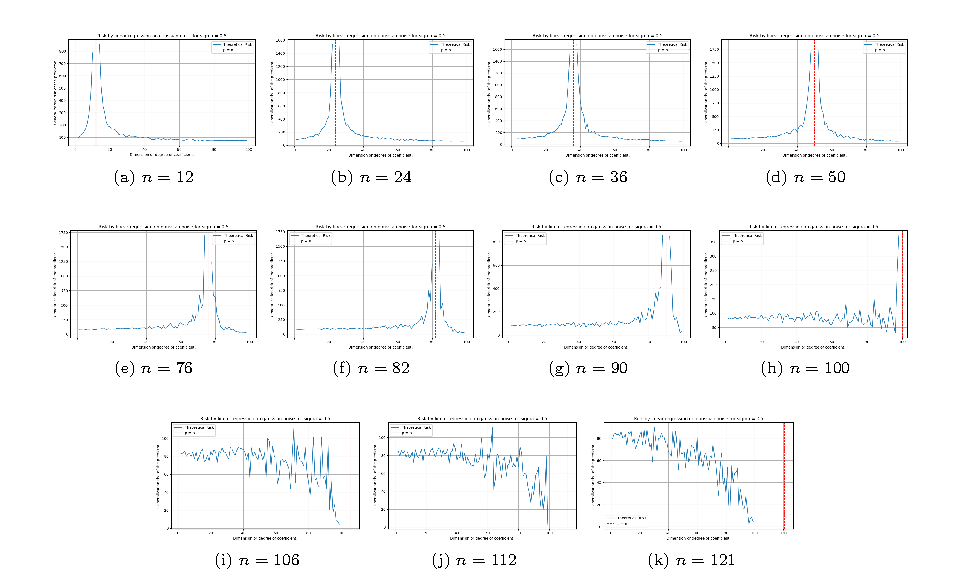
\includegraphics[width=0.8\textwidth]{pdf/theorem_1.pdf}
    \caption{Theorem~\ref{thm:double_descent_lr} behaviours on randomized setting. For this model, we have $d=100$, $\sigma = 0.5$, and variational $n$. Full test cases are for $p=[1,100]$, $n=\{12,24,36,50,76,82,90,100,106,112,121\}$ accordingly. The test function of the concept itself is the same linear model, but with different input only.}
    \label{fig:theorem_double_descent_fig}
\end{figure}

As we see from this particular experimental result, the theorem predicted a loose, left-peak absent, double descent curve estimation for a variety of test case with more and more samples in increment. There exist some fundamental conclusion that we have about the shift of the interpolation threshold upon to $p=n$, which is reflected in the piecewise prediction. However, this pattern breaks down for $n$ higher than specific constant, for this case, starting from $n\approx 100$ to beyond. From here, at least from testing scenario, the test indicates that predictions suggest a breakdown of the double descent estimation. Beyond this, a simple semi-chaotic convergences is observed, from $n=106,112, 121$. 

Interestingly, verifying this notion of easy enough to simplify it into what the statement holds under particular notion. Namely, as we find out, the above double-descent replicating formula can actually be realized by the parameter-wised error, comparing the parameter between the least-square solution and the actual concept. The formula for this is expressed by the exposed MSE on parameter function, for $\beta_{p,k}$ the coefficient value estimated for the $k$-th selected feature when the model is restricted for randomization of $p$ features, 
\begin{equation}
\mathrm{MSE}_{\mathrm{param}}=\left\lvert \hat w - w \right\rvert _{2}^{2}=
\sum_{j=1}^{d}
\left(
  \hat w_{j} - w_{j}
\right)^{2}
\end{equation}
where $\hat w_{j}$ is chosen such that it is equal $0$ for $j \notin S$, otherwise $\beta_{p,k}$ for \(S=\{i_1,\dots,i_p\}\) is the set of selected feature indices. Nevertheless, it is then found dubious why this is true, as for the original statement of \cite{lafon_understanding_2024} indicates correlation to the prediction error of the result, $x^{\top}\hat{w}$ instead. The result of evaluating $\mathrm{MSE}_{\mathrm{param}}$ is presented in Figure~\ref{fig:theorem_double_descent_fig2}.

\begin{figure}[htb]
    \centering
    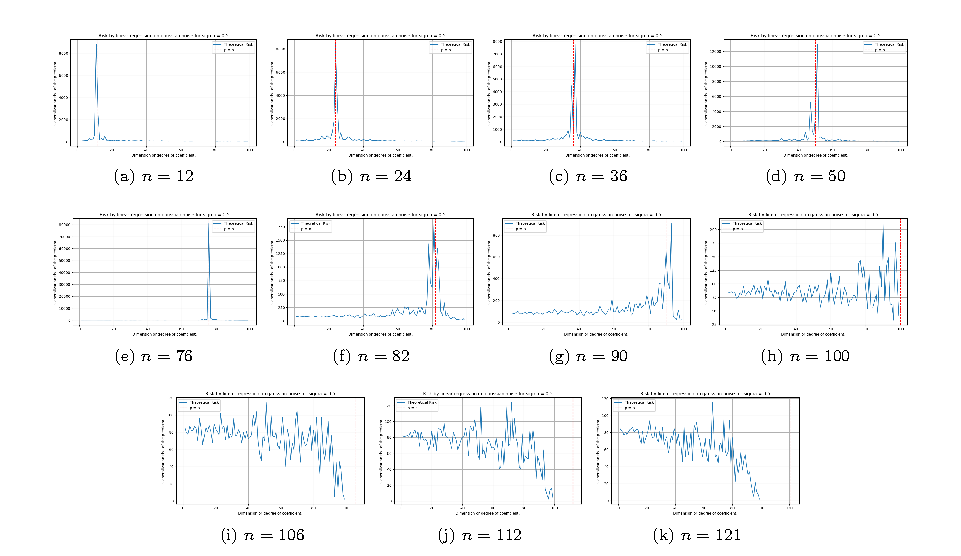
\includegraphics[width=0.8\textwidth]{pdf/theorem_2.pdf}
    \caption{Contrary to Theorem~\ref{thm:double_descent_lr}, this is the behaviours on randomized setting for standard parameter-wised mean square error measure (MSE-on-parameter). For this model, we have $d=100$, $\sigma = 0.5$, and variational $n$. Full test cases are for $p=[1,100]$, $n=\{12,24,36,50,76,82,90,100,106,112,121\}$ accordingly. The test function of the concept itself is the same linear model, but with different input only.}
    \label{fig:theorem_double_descent_fig2}
\end{figure}

If, however, we turn our attention to the statement itself, of which refers to the prediction error $\mathrm{MSE}_{\mathrm{pred}}$, defined by the equation
\begin{equation}
\mathrm{MSE}_{\mathrm{pred}}
=
\frac{1}{n}
\left\lVert
  y - X_{p}\,\hat\beta
\right\rVert_{2}^{2}
=
\frac{1}{n}
\sum_{i=1}^{n}
\left(
  y^{(i)} - x_{p}^{(i)\,T}\,\hat\beta
\right)^{2}
\end{equation}
on $h$ and $c$ accordingly, a strong case of this happens to be not following the pattern indicted by the theorem. Rather than being the interpolation point of return, $p=n$ is now the convergence point of the prediction error instead. Test result is shown in Figure~\ref{fig:theorem_double_descent_fig3}.

\begin{figure}[H]
    \centering
    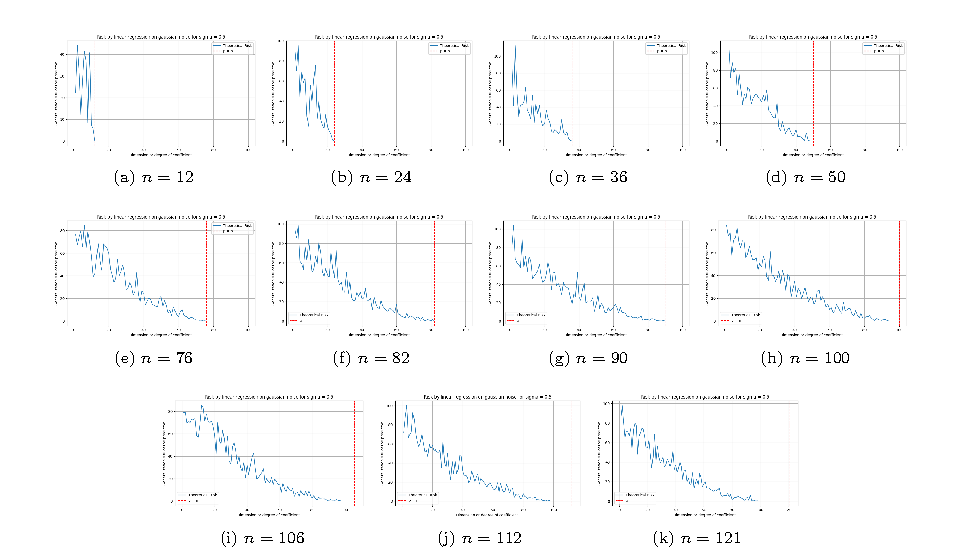
\includegraphics[width=0.8\textwidth]{pdf/theorem_3.pdf}
    \caption{Contrary to Theorem~\ref{thm:double_descent_lr} and both figure~\ref{fig:theorem_double_descent_fig2}, this is the behaviours on randomized setting for standard parameter-wised mean square error measure (MSE-on-prediction). Especially, we do not see double descent pattern in this setting, as it is. For this model, we have $d=100$, $\sigma = 0.5$, and variational $n$. Full test cases are for $p=[1,100]$, $n=\{12,24,36,50,76,82,90,100,106,112,121\}$ accordingly. The test function of the concept itself is the same linear model, but with different input only.}
    \label{fig:theorem_double_descent_fig3}
\end{figure}
\begin{figure}[H]
  \centering
  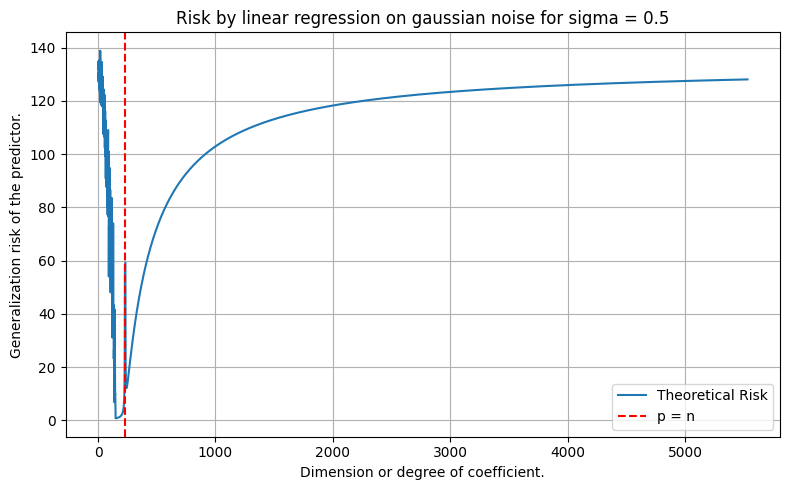
\includegraphics[width=0.6\textwidth]{media/dimensional_descent.png}
  \caption{Similar experiment according to setting and result of Theorem~\ref{eq:linear_gaussian_erm}, where $p$ is in the range [1,5523]. Here, we can see small double descent modelled exactly at the interpolation threshold, while the later region exhibit similar phenomenon as bias-variance tradeoff.}
  \label{fig:contrarian}
\end{figure}
Thence, the theorem gives us two things - the interpolation point, in this setting, refers to the parameter error for their double descent behaviour. However, on the prediction results' error measure, the interpolation point correlates to the point where the defined generalization risk in such case equals zero. These patterns hold up to certain point. However, the test case is only up to $d=p$. An unexplored test case for $p>d$ indicate the surprising fact according still, to the theorem: the generalization risk takes double descent as a region with disturbance in the middle, but bias-variance appears afterward. This is illustrated in Figure~\ref{fig:contrarian}, where the same theorem is applied but in the domain which is usually called as \textit{overparameterized region}. 
\subsection{Linear function class extension}

The current theory prompted for a more general treatment of the linear function class, as in-line with exploring reasonable existing alternatives in interpretation (\cite{nakkiran2019datahurtlinearregression}).

Let us states some hypothesis about the previous experimental cases. First, is the lack of the begin-tail of the prediction on double descent of linear random cutoff features model. This can be explained informally as to be resulted from the uniformity of the operating space. Specifically, all parameters of the $\mathbb{R}^{n}$ parameter space, with respect to the dual space on such $f:\mathbb{R}^{n}\to\mathbb{R}$ projection is defined, are of the same order of magnitude. That is, for $f_{i,k}(x),f_{j,k}(x)$ of arbitrary parameter indexing on the set $k$ of shared parameter choice, and $i\neq j$ being the distinct choice, then we say $f_{i,k}(x)=\mathcal{O}(f_{j,k}(x))$ of the growth of both function on value ranges. Approximately speaking, the choice of parameter does not dramatically growth to a point of no return, like in later examples of polynomial approximation model. Such special model of multi-variable linear projection of scalar output also reinforces the numeric growth of the numerical encoding expression on the hypothesis model. The behaviour of the MSE-on-parameter, the internal risk, is also explainable using the same notion, such is that for a black-box case approximation, such linear model does not allow for average parameter deviation per approximation to be oversaturated and skewed (for example, the degree of polynomial directly counteract this, by separating expressive complexity by growth degree). How such hypothesis can be evaluated, we will have to make it for the general extension experiment, which we will have to conduct. 

Let us define the more general class of linear model, denoted $\mathcal{H}_{L}$, in the following structure of the linear model. We also note that the previous linear class $\mathcal{H}_{p}$ only solves for the problem of underparameterized, hidden parameters $p'$.

\begin{definition}[General linear model]
    Let us define, for $p\in\llbracket1,d\rrbracket$, $\mathcal{H}_{L}$ is the set of functions $h:\mathbb{R}^{d+1}\times R^{q}\to\mathbb{R}^{q}$ of the form: 
    \begin{equation}
        h(\mathbf{u}_{1},\mathbf{u}_{2},\dots,\mathbf{u}_{k}) =  \begin{cases}
            [f_{j}(\mathbf{u}_{1},\mathbf{u}_{2},\dots,\mathbf{u}_{k})]^{\top}\mathbf{w}+b\\
            [(u_{1}u_{2}\dots u_{n})_{j}]^{\top}\mathbf{w} +b & q=1, f_{j}(\{u_{i}\}) = u_{1}\times\dots\times u_{n}\\
            [(u_{1}\odot u_{2}\odot\dots \odot  u_{n})_{j}]^{\top}\mathbf{w} +b & q > 1, f_{j}(\{u_{i}\}) = \mathbf{u}_{1}\odot\dots\odot \mathbf{u}_{n}
        \end{cases}
    \end{equation}
    where $\odot$ is the Hadamard product, and $w\in \mathbb{R}^{d}$ the weight matrix. A subset $\mathcal{H}_{L,p}$ then consists of all set of functions $h$ with $w\in \mathbb{R}^{d}$ having exactly $p$ non-zero elements. 
\end{definition}

Preliminary model learning then will relies on theorem~\ref{thm:double_descent_lr} for its initial prediction, using least square approximation results. The testing is adversarial and consistent, of which we have $c\in \mathcal{H}_{L}$ and $h\in \mathcal{H}_{l,p}$ for $p=d$, which can then further be modified. Because of their equal expressive capacity, respect to independent consideration of the parameter space $\mathbf{X}$, we define the complexity, which will be used later on, simply as \begin{equation}
    \mathbb{C}(h) = \frac{1}{||\overline{\mathbf{x}}-\underline{\mathbf{x}}||}\left[1+p + q + \underset{i\in S}{\mathbb{E}} (w_{i}x_{i})+b\right],\quad S = \{p_{i}\}
\end{equation}
Functional prediction on the classical theorem is presented below, for $n=\{1,\dots,241\}$ samples, and with $p\in[1,200]$. We set the target degree to the maximal 200, since the theorem is not defined on the overparameterized region. 

\begin{figure}[htb]
    \centering
    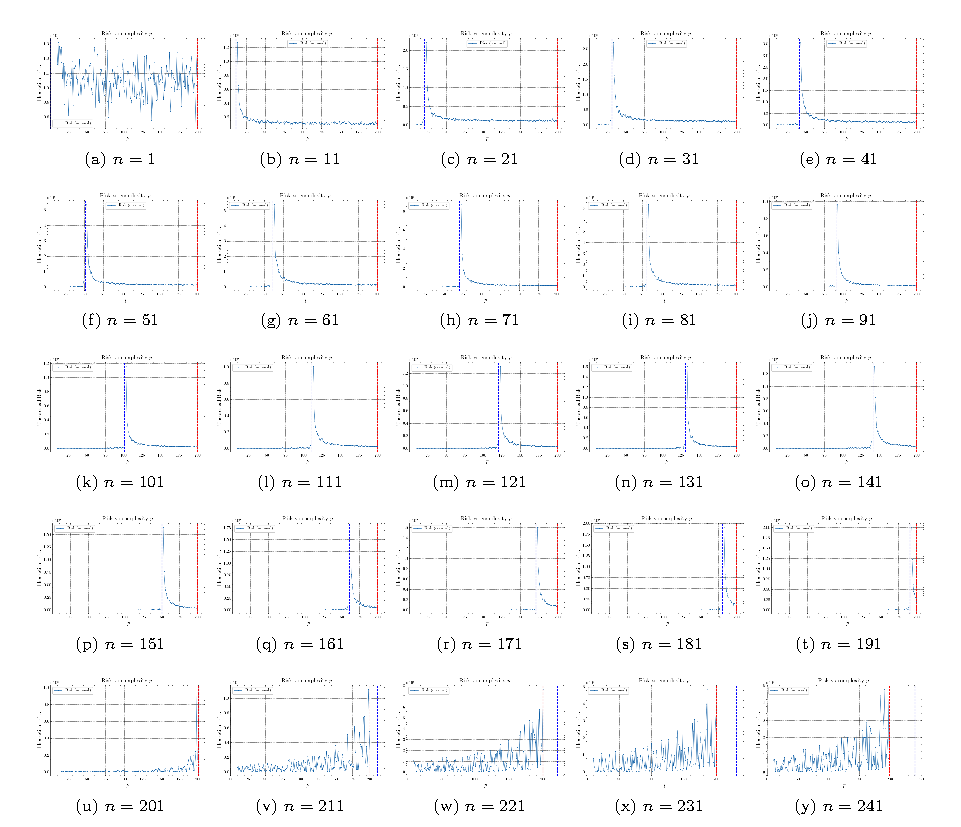
\includegraphics[width=0.8\textwidth]{pdf/linear_gen.pdf}
    \caption{Extension general experimentation, using the prediction made of theorem~\ref{thm:double_descent_lr} for verification.}
\end{figure}

\clearpage

\subsection{Polynomials}

Polynomial space is one of those famous example that is often cited of the bias-variance tradeoff, for example, in \cite{goodfellow2016deep,10.5555/2930837}. Indeed, it is considered, usually, a very effective and high-volatility construct class. Let us reiterate what we know about polynomial class. 

There exists two type of elementary polynomial classification, based on their (i) variable count or (ii) its domain range. We first define the univariate polynomial function.

\begin{definition}[Univariate polynomial]
    A function of a single variable $t$ is a polynomial on its domain if we can put it in the form 
    \begin{equation}
        a_{n}t^{n} + a_{n-1}t^{n-1} + \dots + a_{1}t + a_{0}t^{0}
    \end{equation}
    where $\{a_{i}\}$ are constants, and of a singular variable $t$.  
\end{definition}

From this, we can extend to polynomial of multiple variables. In general, a function $f(x,y)$ is a \textit{multivariate polynomial} in $x,y$ if and only if it can be represented as a finite sum of terms of the form $cx^{k}y^{m}$, where $c$ is a coefficient and $k$ an $m$ are nonnegative integers. The number $k+m$ is called the degree of the term, and the degree of the polynomial $f(x,y)$ is equal to the highest degree of its own terms. We can then generalize multivariate polynomial and univariate polynomial in the same kind. 

\begin{definition}[Polynomial, multivariate generalization]
    Let $K$ be a field. We then denote $K[x_{1},\dots,x_{n}]$ the space of all polynomials in $n$ variables, $x_{1},\dots,x_{n}$. A \textbf{multivariate monomial} is then an expression $x_{1}^{\alpha_{1}}\dots x_{n}^{\alpha_{n}}$ where $\alpha_{1},\dots,\alpha_{n}$ are integers. The degree ò such multivariate polynomial is the largest degree of terms of any monomial term.
\end{definition}
Effectively, we can see that multivariate polynomial can take on many forms, and also unconventional forms. In order to capture any reasonable details, most of the time focus are on symmetric polynomials $f(x,y)$ in which $f(x,y)=f(y,x)$, or homogeneous polynomials in which all the terms are of the same degree. 

Given such, operationally, polynomial is used for expressing other functions, due to their usefulness because of such simplicity and versatility. In fact, applications ranges, even to a polynomial basis on $n$-dimensional space, $(p_{1},\dots,p_{n})\in K[x,\dots,x_{n}]$; their growth rate being polynomial also added more to their strength of approximating fast increasing function, usually expressed and used in setting, for example, polynomial growth class $\mathcal{O}(p(x))$ in computer science. Two applications stand out for such properties: function approximation of arbitrary criteria $\ell$, or polynomial interpolation on arbitrary points. Those two are interconnected, though their objective and object of concern is much different. 

We can define the application of analytical polynomial on arbitrary function by using the criteria on approximation. Usually, this is expressed in the theory of approximation, and requires a guarantee that polynomial can indeed approximate to arbitrary accuracy, of arbitrary function on specific interval. This is the statement of Weierstrass theorem. 

\begin{theorem}[Weierstrass Approximation Theorem]
    Let $f\in C[a,b]$ of all continuously differentiable functions on the closed interval $[a,b]$. Then, for every $\epsilon > 0$, there is a polynomial $p$ such that $||f-p||< \epsilon$, for $||f-p||=\sum_{i=1}^{\infty}|(f(x_{i})-p(x_{i}))|$ \footnote{We again note the disparity between $h(x)-c(x)$ or $c(x)-h(x)$ for clarity. In essence, $c(x)-h(c)$ is looking from the perspective of the concept itself. While $h(x)-c(x)$ is comparison on difference from the perspective of the hypothesis.}
\end{theorem}
Here, $\epsilon$ is defined to be the \textit{global error} of the polynomial with respect to the arbitrary function, and with uniform approximation. Another variation works on the squared error, such that $||f-p||=\sum_{i=1}^{\infty}(f(x_{i})-p(x_{i}))^{2}$, or the mean absolute $$||f-p||=\lim_{n\to\infty}\frac{1}{n}\sum_{i=1}^{n}(f(x_{i})-p(x_{i}))$$
Weierstrass Approximation Theorem provides tighter bound for the mean absolute error, but not the square error, or the mean square case. Nevertheless, they are natural measure on the uniform metric space $C(X)$ with measure $d(f,g)=\sup_{x\in X}|f(x)-g(x)|$. If said metric also use the $L^{p}$ metric instead, which is defined by 
\begin{equation}
    d_{p}(f,g) = \left(\int_{X}|f(x)-f(g)|^{p}\:dx\right)^{1/p}
\end{equation}
we can also see that it is weaker than the bound given by Weierstrass theorem. Generalization of Weierstrass theorem can be made by Stone-Weierstrass theorem instead, of which is state in real space as followed, though generally Weierstrass theorem is sufficed.
\begin{theorem}[Stone-Weierstrass Theorem (real version)]
  Let $S$ be a locally compact Hausdorff space. Let $A$ be the subset of bounded continuous real functions on $X$, or of subalgebras $\mathcal{C}(X,\mathbb{R})$ which contains a non-zero constant function, then $A$ is uniformly dense in $\mathcal{C}(X,\mathbb{R})$ if and only if it separates points. 
\end{theorem}
The setting of polynomial interpolation is rather different from the setting of function approximation. The setting of interpolation gives an $n$ samples set $\mathcal{S}$, of which in this case we restrict to $\mathbb{R}\to\mathbb{R}$. Then, we are required to fit exactly the entire dataset, such that the following setting is sufficed. 
\begin{definition}[Interpolation]
    A function class $\mathcal{F}$ is said to \textbf{interpolate} a distinct dataset $\mathcal{S}_{n}=(x_{n},y_{n})$ of $n$ samples, if there exists $f\in \mathcal{F}$ such that $\mathbb{E}||S_{i}-|f(x_{i})||= 0$. Such $f$ is then called the \textbf{interpolating function} of $\mathcal{S}_{n}$. 
\end{definition}
Under such definition, the question is then if the polynomial class $\mathcal{P}_{n}$ of any given polynomial with the highest degree $n$ is sufficed to approximate such dataset. The answer can be found using unisolvence theorem.

\begin{theorem}[Unisolvence theorem]
    Given $n+1$ bivariate data points $(x_{0},y_{0}),(x_{1},y_{1}),\dots,(x_{n},y_{n})\in \mathcal{S}_{n}\subset \mathbb{R}^{n}$, with all $x_{i}$ distinct, there exists a unique polynomial $p_{n}(x)$ of degree at most $n$ such that $p(x_{i})=y_{i}$ for $i=0,1,\dots,n$.
\end{theorem}

In determining such problem, we can also say that there exists a unique $n$-saddle point function represented here as polynomial, such that to fit $n$ points perfectly by the definition of the saddle point. The process in obtaining such formula is difficult, however, and finding the perfect interpolation polynomial would be computationally significant, and erroneous. 

\begin{definition}[Saddle point,\cite{NieYangZhou2021}]
    Let $X\subseteq \mathbb{R}^{n}$, $Y\subseteq \mathbb{R}^{m}$ be two sets (for dimension $n,m>0$) and let $F(x,y)$ be a continuous function in $(x,y)\in X\times Y$. A pair $(x^{*},y^{*})\in X\times Y$ is said to be a saddle point of $F(x,y)$ over $X\times Y$ if \begin{equation}
        F(x^{*},y) \leq F(x^{*},y^{*})\leq F(x,y^{*}), \quad \forall x\in X, \forall y\in Y
    \end{equation}
\end{definition}

Polynomial regression is one such analytical solution to function approximation task, using Weierstrass theorem as its basis. From such, we can also observe that polynomial regression, and hence polynomial interpolation, are correlated and can be reduced to each other. Polynomial regression can be reduced to interpolation via stating the criteria such that, denoting it as $\ell$, then $\ell(f,p)=0$, and interpolation can be reduced to regression via the condition that $p(x_{i})-y_{i}\leq \epsilon$ for arbitrary $\epsilon>0$. Hence, the regression formulae lie between the two extreme: the Weierstrass setting and the interpolation setting. 

We then have to identify such extreme and what kind of extreme they represent. Fortunately, we know this as the problem of \textbf{transparency}, in the setting of approximation, which certainly correlates to the learning theory. According to such, the Stone-Weierstrass represents the total transparency case, where the function $f$ is known to the approximator with polynomial class. Interpolation represents total black box, where the goal is only to interpolate the sample point by itself. In between such interpretation, there exists a fundamental assumption, hence the structural assumption. 

\begin{assumption}[Transparency]
    For any bivariate pair $(x,y)$, we assume each pair depends on and originate from a based concept $y=f(x)$. 
\end{assumption}

Two kinds of knowledge is then available, which correlates to the degree of freedom the observation space can have. First is the knowledge of $f$. This knowledge of $f$ is encoded directly by the number of sample point and their distribution in certain case. Accordingly, the worst case is as followed. 

\begin{conjecture}
    If $\forall x$ there exists $y$ corresponding to such, and $(x,y)\in \mathcal{S}$, then we say we have total transparency to the concept $f$. If there exists only finite $x$ that we can have $y$ corresponding to, then we say we have limited transparency to the concept $f$. If we assume no knowledge of $f$, then we say the setting is called the \textbf{black-box setting}. 
\end{conjecture}

Secondly is the action on the dataset itself. One of the main assumption that is usually observed is that 

\begin{assumption}[Fallacy]
    We assume every bivariate pair $(x_{i},y_{i})\in f[\mathcal{S}_{n}]$, such that $f(x_{i})=y_{i}$. 
\end{assumption}

However, usually, this is not the case, as we have \textbf{noise} in addition from the dataset. The origin of the noise cannot be tracked. However, we can interpret what happens when such noise is introduced to the dataset. The noise transitions the transparency of the learned setting, on the field $\mathbb{R}$, by utilizing the dense property of the real space. Assuming we operate on $\mathbb{Z}$. Then, each discrete noise will introduce abnormality point such that no function on $\mathbb{Z}$ will be able to match, up to certain distance on $\mathbb{Z}$. This is because on such space, there exists no point $x_1, x_{2}$, for example, that lies between $d(x_{1},x_{2})=1$. If the noise is randomized on $\pm 1$, then there will exists no function that can approximate such disparity better than a random fluctuating function. However, on $\mathbb{R}$, the real number is inherently dense, such that there will always be certain point $x_{3}$ such that $x_{3}\in [x_{1},x_{2}]$, by the density of real number. By the distance metric on $\mathbb{R}$, we define $d(X,Y)=|X-Y|$ for distance between two data points. Noise intrinsically increases such distance, such that $d'(X,Y)> d(X,Y)$. Hence, the space in which density can appear increase, thus there then exists more fluctuation, and thus more uncertainty between such two points. This notion can be increased from local uncertainty to global uncertainty, hence the \textit{noisy dataset}. 

We then can measure or aggregate some properties of the dataset itself, including the \textbf{uncertainty} of the dataset. We define the simple uncertainty of the dataset as followed. 

\begin{definition}[Dataset uncertainty]
    Given a closed interval $[a,b]$, for the sample set $\mathcal{S}_{n}=(X,Y)\in [a,b]$, the uncertainty $\mathcal{U}(\mathcal{S}_{n})$ is defined as 
    \begin{equation}
        \mathcal{U}(\mathcal{S}_{n}) = \left[ \underset{x_{i}\in X}{\mathbb{E}}\Big( x_{i+1} - x_{i} \Big)^{2} + \underset{y_{i}\in Y}{\mathbb{E}} \Big( y_{i+1}- y_{i} \Big)^{2} \right]^{1/2}
    \end{equation}
    We assume $X,Y$ are totally ordered sets. 
\end{definition}
Hence, the assumption of fallacy assumes $\mathcal{U}(\mathcal{S}_{n})=0$, though in reality it is often $\mathcal{U}(\mathcal{S}_{n})>0$. With this, we can quantify how the dataset is behaving on the scale of the bivariate form typically seen. Noise intrinsically increases this distance, usually by the $y$-axis. This dataset uncertainty increases with multivariate dataset, for example, $(\mathbf{x},y)$ of $\mathbb{R}^{n}\to\mathbb{R}$. We call the new metric as the \textit{empirical uncertainty metric}.

Thirdly, is the treatment on such information. Even though information is known, such as from the assumption of transparency and the fallacy conjecture, it relies on the method in which the model uses that make use of such information. Polynomial interpolation effectively removes information about transparency, and thus the interpolation setting is a kind of \textbf{black-box absolute setting}. This setting is \textit{extremely brittle}, as to see that if $y_{i}$ is slightly wrong due to measurement noise, the interpolant oscillates wildly, which is explained by Runge phenomenon (\cite{Runge1901,CorlessSevyeri2018,AMC2009RungeDivergence}). Probability then arises from such setting naturally, though this particular degree of probabilistic setting must be quantified, which comes from the process that the model simulates upon. Regression is inherently not probabilistic, but treatment about the probabilistic assumption, for example, such that $(X,Y)$ inherently as random variables. We can then separate this into three parts - the data-level probabilistic layer (data uncertainty), the model-level layer, and the algorithm-layer that determines the solution solver within such model. We can define that as followed. 

\begin{definition}[Probabilistic layer]
    Given a learning setting with dataset $\mathcal{S}$ of bivariate pairs, $h\in \mathcal{H}$, $c\in \mathcal{C}$ as the hypothesis and concept, we have the following conceptual probabilistic setting:\footnote{Currently, we have no way to \textbf{quantify} the `probabilistic degree' of the system setting itself}
    \begin{enumerate}[leftmargin=2cm,itemsep=1pt,topsep=1pt]
        \item Data-level probability: Sampling assumptions (observation sample points) such that there exists the distribution $\mathcal{D}\sim (X,Y)$, intrinsic data uncertainty $\mathcal{U}(\mathcal{S}_{n})$. 
        \item Model-level probability: Structure of the dataset is controlled by the concept structure $\{\theta\}\in c$, $c$ is modelled as a target sampler $c\equiv \mathcal{D}$, knowledge about the structure of $c$, Bayesian prior-posterior assumptions, $\mathbb{P}(Y\mid X, \{\theta\})$. For Bayesian polynomial regression, the model-level probability is formulated as \begin{equation}
            \mathbb{P}(Y\mid X) = \int \mathbb{P}(Y\mid X,\theta)\mathbb{P}(\theta)\: d\theta, \quad \mathbb{P}(\theta_{j}) = \mathcal{N}(0,\sigma^{2})
        \end{equation}
        of which assumes aleatoric uncertainty and epistemic uncertainty from the weight. 
        \item Algorithm-level probability: Stochastic method, decision conditional (dropout, MCMC), ensembles criteria, Monte-Carlo initialization, variational inference. 
    \end{enumerate}
\end{definition}

Dynamically, in this paper, we would like to investigate this particular junction between uncertainties, to see what happens when the model transparency, the treatment of data, and so on, that exhibits the observations that we would receive from the model itself. The experimental details will infer such result. 

Generally, we would be entitled to see particular trajectory specifically designed around the point of interpolating match, or $n=m$ of $n$ degree of freedom, technically, and $m$ data points. After this point, there exist two possibility of dynamic - either the model dilutes, in which case result in \textit{double descent}, or the model fluctuate strongly afterward, leading to \textit{bias-variance emergence} again later on. This conclusion however, would have to be analysed within the current framework of the possible interjection to its fluctuation strength. For example, in the monomial basis $\{x^{i}\}^{n}$, any given fluctuation contributes to the entire polynomial. In such case, fluctuation of the other $[0,n-k]$ of arbitrary $k$ and large enough $n$ would be unaccounted for by the scale. Conversely, restrict them to $[1,0]$ range will reveal something about the system, however will destroy particular properties of the prediction, which is not recommended. Nevertheless, we must conduct the test before giving in any reasonable conclusion.

Previously, we said that we did indeed focus on the interpolation problem. Now, assuming we have given the interpolating algorithm $\mathcal{A}$ to approximate the interpolation, what will this look like? Firstly, solving this is \textit{very computationally expensive}, because it is a dense, $(n+1)\times(n+1)$ linear system, and even more so if we consider the overparameterized outcome. However, this can be reduced further down if we attempt to solve them using convergence bound, but will be still very expensive. That and incremental soft interpolation is somewhat out of the question since it will be kind of the same. Aside from the insight, we would still have to know what to do. Then there exists two ways - we have some version of this to optimize of simply evaluating by gradient descent optimization, or, we can use somewhat analytical fit for the case of soft interpolation modification. 

A theory on such problem can be obtained of its mechanics, as will be a fairly intuitive way in consideration of the theory of interpolation, as well as the technique of interpolation by itself. For a fixed-range interpolation threshold problem, a hard-encoded interpolation solution requires $n$-degree polynomial, of which has $n+1$ degree of fitness, to fit $n+1$ distinct points. Suppose all points are distinct of the set $S$ which is finite, then this is the case. If we switch to the problem of interpolation but induce a more forgiving bound, there exists a possibility that it induces a relative \textit{density averaging path} for the points, especially if we are considering the case where $p>n$ for $p$ saddle points or degree of fitness, and $n$ the number of point to interpolate. In a more nuanced formulation, we have

\begin{equation}\label{eq:soft_hard_interpolation_role}
\mathsf{Flatten}\left(\begin{bmatrix}
1 & x_0 & x_0^2 & \cdots & x_0^p \\
1 & x_1 & x_1^2 & \cdots & x_1^p \\
\vdots & \vdots & \vdots & \ddots & \vdots \\
1 & x_p & x_p^2 & \cdots & x_p^p \\
\vdots & \vdots & \vdots & \ddots & \vdots \\
1 & x_n & x_n^2 & \cdots & x_n^p
\end{bmatrix}_{n\times p}
\begin{bmatrix}
a_0 \\
a_1 \\
a_2 \\
\vdots \\
a_p
\end{bmatrix}
- 
\begin{bmatrix}
f(x_0) \\
f(x_1) \\
f(x_2) \\
f(x_3) \\
\vdots \\
f(x_n)
\end{bmatrix}\right)
\leq \epsilon
\end{equation}
or equivalently, $\mathsf{Flatten}(\mathbf{X}_{n\times p}\mathbf{w}_{n}-\mathbf{Y}_{n})\leq \epsilon$ where $\mathsf{Flatten}(\cdot)$ is the compression of vector to scalar, or so $\mathsf{Flatten}: \mathbb{R}^{n}\to \mathbb{R}$. This essentially is the problem of solving $n$ points approximation, toward using only $p$ saddle points available. If $\epsilon =0$, it is well known that interpolation is impossible. However, if $\epsilon\ne 0$, there are possibilities, depends on the shape of the dataset, that there will exist a data-dependent property or more that indict a particular \textit{density preference} toward those saddle points - or rather, the act of density averaging. This is reflected rather implicitly in the structure itself. In machine learning, the error measure is usually the mean average, such is to say that the criterion now would look more like $\mathbb{E}\Big[\mathsf{Flatten}(\mathbf{X}_{n\times p}\mathbf{w}_{n}-\mathbf{Y}_{n})\Big]\leq \epsilon$. Formally, we have the following hypothesis

\begin{hypothesis}[Polynomial double descent]\label{hyp:hypothesis_poly_dd}
For a polynomial $\{a_{i}x^{i}\}_{n}$ on Vandermonde basis, approximating on the set $\{(x_{k},y_{k})\}_{m}$, then
\begin{enumerate}[topsep=1pt,itemsep=1pt]
  \item For $n<m$, we expect the polynomial form factor to be \textit{inherently sparse}, such that for an iterative approximation, for each $p_{i}$ saddle point of the polynomial expansion form, there exists an $\epsilon$-ball $B_{\epsilon}$ for $\epsilon>0$ with at least one data point satisfying $(x_{k},y_{k})\in B_{\epsilon}$. 
  \item For $n=m$, we expect the polynomial to be able to fit all points, up to hard interpolation threshold such that $\hat{R}_{S}\approx 0$. 
  \item For $n>m$, we expect the polynomial form factor to be \textit{locally dense} then turning to \textit{globally dense}, over random ensembles. That is, for every point $(x_{k},y_{k})$ there exists a $\beta$-ball $B_{\beta}$ such that there is at least one saddle point of the polynomial belong to the ball. 
\end{enumerate}
\end{hypothesis}

The shift that will be hypothesized to appear here is expected to be from sparse in the polynomial term sense, out to globally dense with enough model complexity, over an iterative process. One also main point of clarity is, at certain point right now, we haven't discovered the effect of error deviation, yet. For such, I theorized the following. 

\begin{conjecture}[Double descent]
  Double descent happens, for a polynomial class model $h_{n}\in\mathcal{H}_{p}$, is upper bounded to certain error deviation $\epsilon>0$ from the mean only of the generalization (test) dataset verification. 
\end{conjecture}

\begin{figure}[htb]
    \centering
    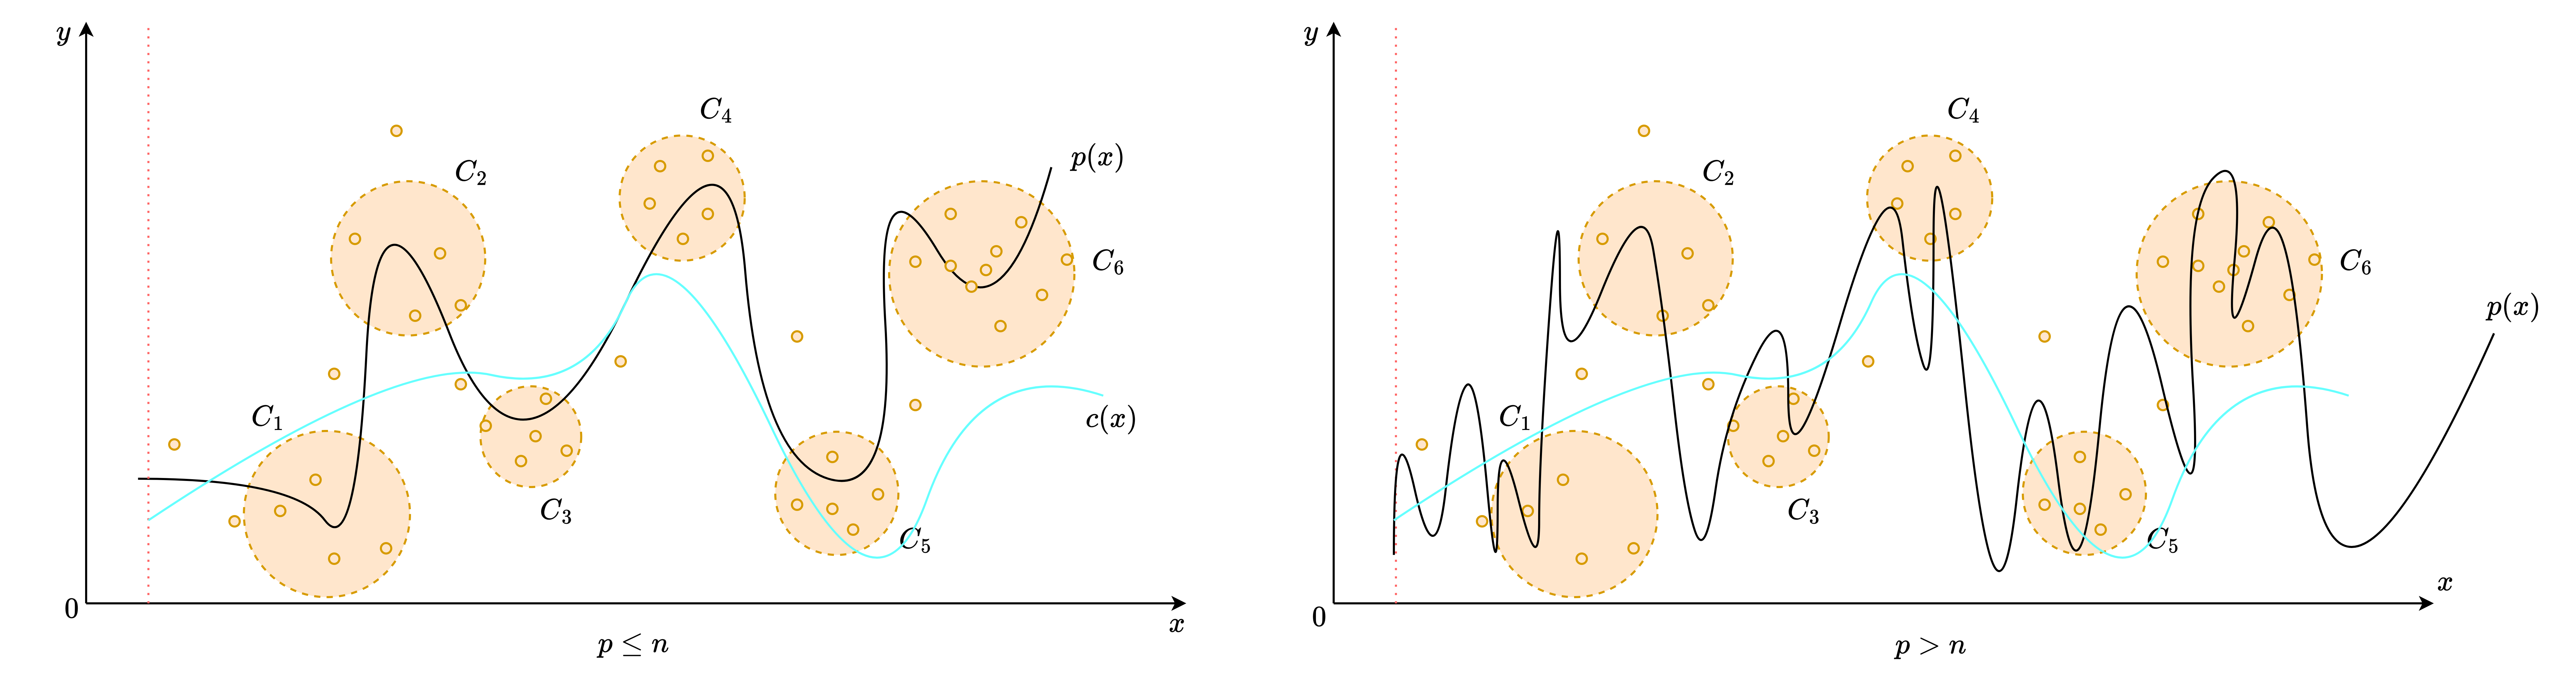
\includegraphics[width=1\textwidth]{diagram_poly_dd.png}
    \caption{Intuition of Hypothesis~\ref{hyp:hypothesis_poly_dd}. Effectively, in the overparameterized range $(p>n)$, the problem turns into soft interpolation, where the polynomial is possible to be dense enough such that relative error remains internally low. This can also happen if the dataset itself is intrinsically large.}
\end{figure}

That is, the disparity between the test and training dataset helps in such regard. If the two dataset is partitioned in the sense that their deviation is practically the same (which can be done using synthetic generation for a control group), then this will amount to not much of it. After all, it will be the consequence of the algorithm and error landscape interpretation used. 

For this, we propose another speculative observation beside such, as to consider adjourned transform of the Vandermonde basis to the Newtonian or similar basis, in which the effects and motion can be easily observed, as least easy. This is because aside from mapping down to $[-1,1]$, normal polynomial on monomial basis gives suboptimal result because of intrinsic high-degree term domination. 

This will become more relevant later on in the analysis. 

\subsubsection{Polynomial model structure} 

Now, for mathematical analysis and experimental design, we would like to state the current main structure of a polynomial model. Specifically, in such example, we are concerned of the shallow polynomial neural network, of which is stated as such in \cite{arjevani2025geometryoptimizationshallowpolynomial}. Notice that it is defined on the normal Vandermonde basis, where an expression of such polynomial model under Newtonian or Lagrangian basis is not so clear-cut of an analysis.  

\begin{definition}[Shallow polynomial neural network]\label{def:poly_structure1}
    A shallow polynomial is a neural network of one layer that are functions $f_{\mathcal W}$, defined such as:
$\mathbb R^d \rightarrow \mathbb{R}$ of the form
\begin{equation}\label{eq:network_model} f_{\mathcal W}(x) = \sum_{i=1}^r
\alpha_{i} (w_i \cdot x)^d, \qquad \mathcal W = (\alpha,w_1,\ldots,w_k) \in
\mathbb{R}^r \times (\mathbb{R}^{n})^k,
\end{equation} 
where $d \in \mathbb{N}$.
\end{definition}
A modification is then available. 
\begin{definition}[Polynomial neural network, testing]
    The polynomial network based on Model~\ref{def:poly_structure1} is modified as 
    \begin{equation}
        f_{\Theta}(x) = \sum_{i=1}^{d} \theta_i \left( \mathbf{w}^\top x \right)^i + b, \quad \Theta = (\{\theta_{i}\},\{w_{k}\},b)
    \end{equation}
\end{definition}
We then can state the model within a testing scenario listed as such, to fully capture the structural foundation of the related testing model class. For the notion of complexity, naively, we employ two kinds of complexity measure. First is the usual complexity measure via parameter counts. Second, is the expressive complexity on the basis of the linear transformation space. That is, an expressive complexity that take into account the fact that $\mathcal{O}(wx^{n})$ will always be stronger than $\mathcal{O}(wx^{n-1})$ for $x>1$. We have the following definition of such complexity in simple term. 

\begin{definition}[Polynomial expressive complexity]
    For $x>1$ or $\mathbf{x}_{i}>1$ of $\mathbf{x}\in\mathbb{R}^{n}$ as input. Denote the polynomial class as $\mathcal{P}_{n}$ of their highest degree $n$, then we define the total expressive complexity of $p\in \mathcal{P}_{n}$ as followed.
    \begin{equation}
\mathbb{C}_{E}(p)
= \mathbb{E}\!\left[
\|\alpha\|_{d} + 1
+ \frac{\sum_{i\in S\setminus\{p_{n}\}} w_i\,i}{\|p\|-p_{n}}
+ \frac{1}{||\overline{x}-\underline{x}||}\!\left(
\frac{\sum_{i\in S} i}{\|p\|} + w_{n}n
\right)
\right],
\end{equation}
    where $S=\{p_{j}\}$, $||p||$ denotes the amount of different degree separable terms and $||x_{max}-x_{min}||$ is the observable range of the dataset. 
\end{definition}
The first term is the normalized linear parameters $\theta_{i}$ fixing and controlling the shift of the polynomial inning parameter, the second term is the sum of weight-aware complexity with degree factor, and the degree factor over operating range $||x_{max}-x_{min}||$ of the dataset, for the degree complexity. The final term is the last weight-aware complexity for the dominating degree $n$ of the polynomial function. 


\subsubsection{Testing result}
The testing scenario will be as followed. The following set of parameters are required for controlling the testing case, aside from different system measures. 

\begin{table}[htb]
  \centering
  \footnotesize
  \begin{threeparttable}
    \caption{Controllable parameters and hyperparameters for polynomial class analysis}
    \label{tab:polynomial_test}
    % three columns: adaptive widths
    \begin{tabularx}{\textwidth}{@{} L{0.25\textwidth}
                                     L{0.2\textwidth}
                                     >{\RaggedRight\arraybackslash}X @{}}
      \toprule
      \textbf{Information} & \textbf{Notation} & \textbf{Details} \\
      \midrule
      Hypothesis model
        & $h[\mathcal{W}_{h},\mathbf{H}_{h}]\in \mathcal{H}$
        & Hypothesis model. For simplicity, it contains $\mathcal{W}$ as the configuration parameter set, and $\mathbf{H}$ the fixed hyperparameters \\
      \addlinespace[1pt]
      Concept model
        & $c[\mathcal{W}_{c},\mathbf{H}_{c}]\in \mathcal{C}$
        & Concept or target model. Similar configuration as the hypothesis model \\
      \addlinespace[1pt]
      Complexity measure(s)
        & $\{\mathbb{C}(\cdot)\}$
        & Set of complexity measure of choice for any arbitrary model taken in. \\
      \addlinespace[1pt]
      Sample count
        & $m$
        & The number of sample available for hypothesis model of $c$, for $m=|\mathcal{S}|$ dataset\\
      \addlinespace[1pt]
      Hypothesis dimension (hyperparameter)
        & $[d_{h}]$
        & An explicit hyperparameter contains the list of all in-testing polynomial degree for the hypothesis model. \\
      \addlinespace[1pt]
      Concept dimension (hyperparameter)
        & $d_{c}$
        & An explicit hyperparameter of the concept's true dimension. Theorized such that $d_{c}=d_{h,i}$ for arbitrary $i$ will reduce to possible low-error problem.\\
      \addlinespace[1pt]
      Data noise
        & $\epsilon_{\mathcal{S}}$
        & Dataset-wide noise with relative strength to the value of the sample point. This is to reduce vanishing noise with higher-degree polynomial sample points. \\
      \addlinespace[1pt]
      Learning parameters
        & $\mathrm{epoch}, lr, \mathrm{bs}$
        & Two main parameters for gradient-descent, iterative-based algorithm - the epoch, the learning rate, and the batch size.\\
      \bottomrule
    \end{tabularx}

    \begin{tablenotes}
      \footnotesize
      \item[] \textbf{Notes:} We output to $\{\mathbb{E}[\ell]\}$ as the expected value of the error measure on $h,c$. There are a few things possible, but under approximatio setting, we use MSE-on-parameter and MSE-on-prediction for two different insights: internal representation and external representation. 
    \end{tablenotes}
  \end{threeparttable}
\end{table}

We note a few problems with both interpolation interpretation and polynomial regression of higher-degree terms. Firstly, is the intrinsic interpolation error and numerical, software issue error. Higher degree polynomial can be represented as solving for a wide Vandermonde system of $n$ degrees for $m$ sample points. Using monomial basis for interpolation, either for soft interpolation also exhibits instability and numerical garbage within the operations, as indicated by \cite{Shen_2025}. They can also be a potential source of double descent, as the majority of models tested around this range are not coded effectively for handling large data operations as such, and artifacts from such choices might be taken as the indication of double descent in some particular cases. 

\clearpage

\subsection{Support Vector Machine}

Support vector machine, first formally originated from \cite{Vapnik1999-VAPTNO}, is a model inherently, specifically defined for pattern recognition task, and binary classification via an \textit{optimal separating hyperplane}. There are two variants for SVM, namely, for linear and nonlinear hyperplane. 

\subsubsection{Introduction}

The SV machine implements the following two precursor ideas: It maps the input vectors $x$, supposed of the setting, into a high-dimensional feature space $Z$ through some nonlinear mapping, chosen a priori. In this space, an optimal separating hyperplane is constructed. By statistical learning theory, Vapnik restricted the function class (as for infinite hypothesis it is impossible to learn) to the class of hyperplanes by 
\begin{equation}
    \langle \mathbf{w}\cdot \mathbf{x} \rangle + b = 0 ; \quad \mathbf{w}\in \mathbb{R}^{n} , b\in \mathbb{R}
\end{equation}
which $\mathbf{w}$ is the controlling weight, $\mathbf{x}$ is the input space to the space of all binary $\{-1,+1\}$ category. Hence, this basically divide the input space into two: one part containing vectors of the class $-1$ and the others being $+1$. If there exists such a thing, then it is said to be \textit{linearly separable}. To find the class of a particular vector $\mathbf{x}$, we use the following decision function 
\begin{equation}
    f(\mathbf{x}) = \mathrm{sgn}[\langle \mathbf{w}\cdot \mathbf{x}\rangle+ b]
\end{equation}
This is called the \textbf{hyperplane classifier} class. As can be understood simply from such, there exists many hyperplanes that can correctly classifies the classes. It has been then shown that the hyperplane that guarantees the best generalization problem performances is the one with the maximal margin of separation between two classes (\cite{Cristianini2000AnIT}). The above form of finding final classification can then be presented in dual form, which then depends only on dot products between vectors, as 
\begin{equation}
    f(\mathbf{x}) = \mathrm{sgn}\left(\sum^{\ell}_{i=1} y_{i}\alpha_{i} \langle \mathbf{x}\cdot \mathbf{x}_{i} \rangle+ b\right)
\end{equation} where $\alpha_{i}\in \mathbb{R}$ is a real-valued variable that can be viewed as a \textit{measure} of how much informational value $\mathbf{x}_{i}$ has (for $x_{i}$ the support vectors we get from training)\footnote{The \textit{support vector} of a particular hyperplane $\mathbf{y}$ is the collections of all points that lies closest to the hyperplane, which is specified as condition for maximization on both side of maximal margin vector machine.}

The second idea is of the \textit{kernel method}. This particular method, useful and well-known of the time SVM was created, gain a more prominent position among other techniques, including neural network. Specifically, this method is characterized by the mapping of the input vectors into a richer (usually high-dimensional) feature space where they satisfy \textit{linear separable} criteria. This prompted the possibility to solve nonlinear problem through such mapping, and indeed yields a nonlinear decision surface in the input space, which is linear in the feature space. A \textbf{kernel} (function) is then a function $k(\mathbf{x},\mathbf{y})$ that given two vectors in input space, return the dot product of their images in feature space such that $k(\mathbf{x},\mathbf{y})=\langle \phi(x), \phi(y) \rangle$ for the nonlinear mapping $\phi$. The general form of SVM is then 
\begin{equation}
    f(\mathbf{x}) = \mathrm{sgn} \left(\sum^{\ell}_{i=1} y_{i}\alpha_{i}k\langle \mathbf{x}\cdot \mathbf{x}_{i} \rangle\right)
\end{equation}
for any particular final categorization. One of the major problem for analysing SVM, is in the properties of it potentially having infinitely many parameters, depends on the size of the dataset. This makes the curve of both bias-variance and double descent not applicable in such regard - infinitely many parameters complexity, yet still finite complexity class. 

From such observation, it would seem imperative that the notion of complexity based solely on the parameter counts of certain model construction is ill-equipped for certain flavours of machine learning model, in this case support vector machine (in the same type is the Gaussian Mixture Model). No double descent has been observed by empirical reports record per the author's knowledge. 



\clearpage

\section{Axiomatic formalization}

Concurrent theories are inherently unstable and with many variations, making them ill-suited for instant application on analysis of different models without losing major information about the structural details and expressions. Hence, we propose a novel analysis on the basis of the axiomatization of the learning setting, under various structural assumptions. 

\subsection{Learning theory formalism}



\subsection{Neural network formalism}
Previously, we have been discovering, examining past results and testing on models of different types, generally classical models. While decisive, each modelling setting requires different analysis and is often not so streamline. Hence, we propose a general analysis on the structure of a feed-forward style neural network architecture, as usual, for further analysis and identification. 

A neural network (\cite{goodfellow2016deep,zhang2023mathematical}) $N$ is typically specified by the dual $(L,[S])$ where $L$ is the number of processing layer of a neuron, and $[S]$ is the list of neurons configuration per layer - for example, the number of neurons per layer, and so on. For such network, the definition can be simple as followed 

\begin{definition}[Standard multilayer network, \cite{zhang2023divedeeplearning}]
    We define a $K$-layer fully-connected deep neural network with real-valued output. Let $m^{(0)}=d$ and $m^{(K)}=1$ for $m$ the width of the network, and $d$ the shape of the input vector. We then recursively define: 
\begin{align}
    x_{j}^{(0)} &= x_{j} \quad (j=1,\dots,m^{(0)}),\\ 
    x_{j}^{(k)} &= h\left(\sum^{m^{(k-1)}}_{j'=1} \theta_{j,j'}^{(k)}x_{j'}^{(k-1)}+ b_{j}^{(k)}\right)\quad (j=1,\dots,m^{(k)}), \quad k = 1,2,\dots,K-1\\
    f(x) & = x_{1}^{(K)} = \sum^{m^{(K-1)}}_{j=1} u_{j}x_{j}^{(K-1)}
\end{align}
where the model parameters can be represented by $w=\{[u_{j}, \theta_{j,j'}^{(k)}, b_{j}^{(k)}]: j,j',k\}$ with $m^{(k)}$ being the number of hidden units at layer $k$; $\theta\in \mathbb{R}^{m}$ the weight of the neuron.
\end{definition}

\begin{figure}[htb]
    \centering
    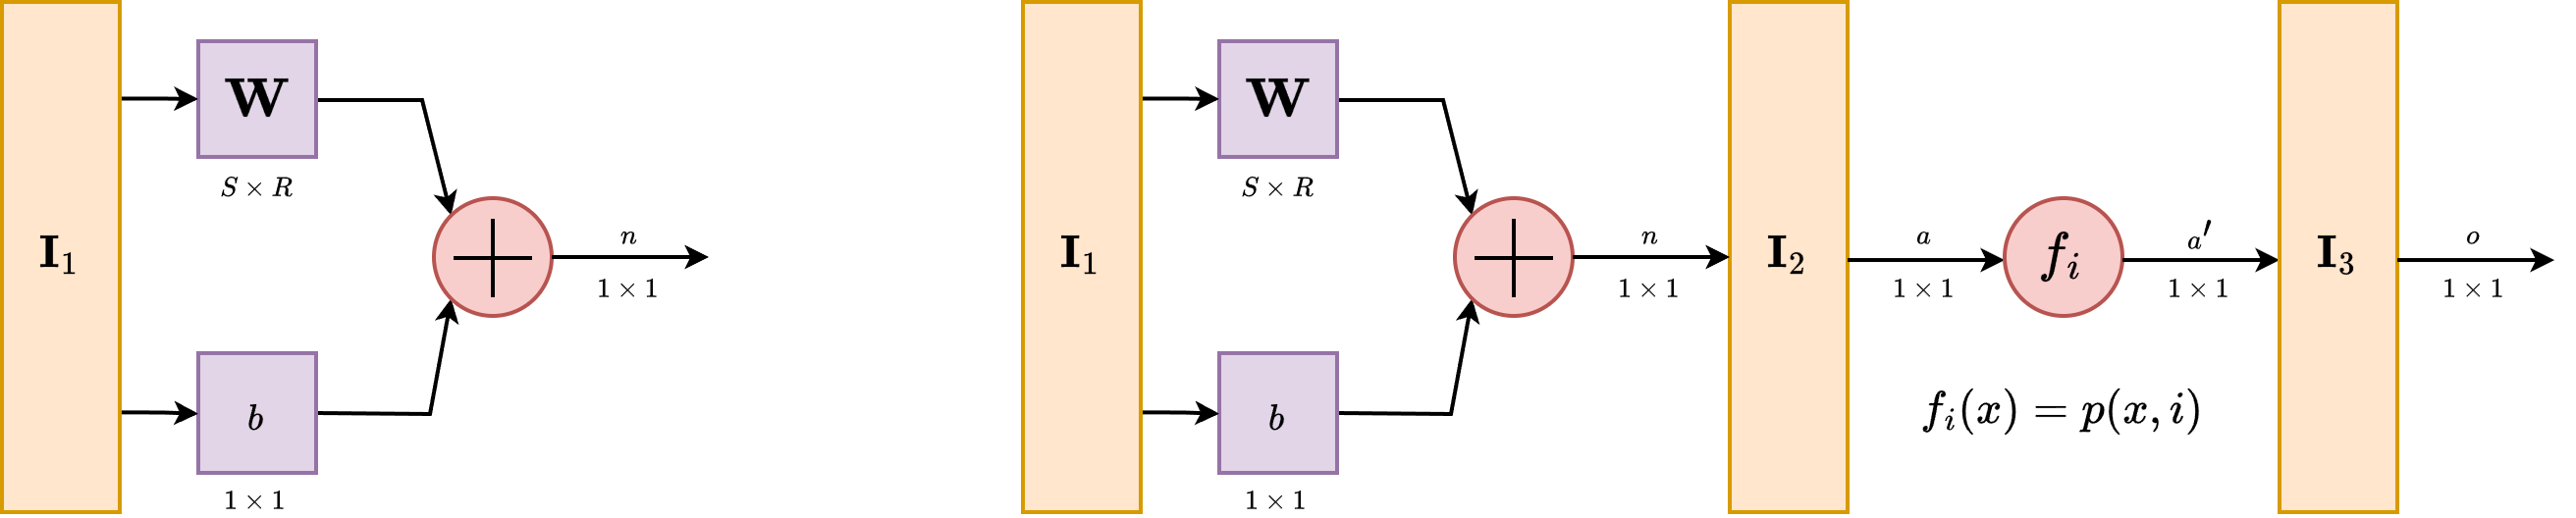
\includegraphics[width=0.9\textwidth]{structure_network_1.png}
    \caption{Flow diagram of the shallow neural network structure in linear and polynomial case, following the notation of \cite{10.5555/2721661} in \textit{Neural Network Design}. The Support Vector Machine flow diagram looks similar to the case of polynomial, except a decision function at the end of the output, and changing the function $f$ into the kernel function $K(x',x)$.}
\end{figure}

Here, each neuron is denoted by their expression as $f(\mathbf{W}^{\top}\mathbf{x}+b)$ for the activation function $f$. We can simplify a lot of those structures above into the neural network schemes. For example, the linear function class case can be simplified to a single $(2,[n,1])$ neural network, such as: 
\begin{align}
    x^{(0)}_{j} &= x_{j} \quad (j=1,\dots,n)\\
    x^{(1)} &= \sum_{j'=1}^{n} w_{j'}x_{j'}, 
\end{align}
without the activation function $h$. The polynomial neural network can be represented by 
\begin{align}
    x_{j}^{(0)} &= x_{j} \quad (j=1,\dots,m^{(0)}),\\ 
    x_{j}^{(1)} &= h\left(\sum^{m^{(0)}}_{j'=1} \theta_{j,j'}^{(1)}x_{j'}^{(0)} \right)+b_{j}^{(k)}\quad (j=1,\dots,m^{(1)}),\quad h(x_{j})=x^{j}\\
    f(x) & = x_{1}^{(2)} = \sum^{m^{(1)}}_{j=1} u_{j}x_{j}^{(1)}
\end{align}
for a neural network of shape $(3,[n,n,1])$, and of polynomial custom scaling function. For support vector machine, this is even harder to do, since its definition varies between different notion of the model itself. However, it is interesting because we can treat it as an arbitrary generation of a neural network structure. There are papers about formalizing SVM in the sense of neural network, including making it to be an infinitely-wide shallow neural network, for example, \cite{chen2021equivalence,wang2019svmdsn,zhang2014equivalence}, however, the structure that is formed from the SVM learner can be expressed as followed:
\begin{definition}[Support vector machine setting]
    For any given optimization problem on input space $x_{i}\in \mathbb{R}^{d}$, and label $y_{i}=\{\pm 1\}$, the shallow neural network resultant from the training procedure is always of the form:
    \begin{align}
        x_{j}^{(0)} &= x_{j} \quad (j=1,\dots,m^{(0)}),\\ 
        x_{j}^{(1)} &= \sum_{j'\in m^{(1)}} \theta^{(1)}x_{j'}^{(0)}K(x_{j'}^{(0)},x)\\
        f(x) & = \sign{(x_{1}^{(2)}) }
    \end{align}
    for a specific kernel $K(x,x')$. 
\end{definition}

Those three fundamental conversions to neural network raise interesting insight into the neural network formalism. For linear and polynomial shallow neural network, we design the network and then provide it with a training scenario, evaluated of the proxy generalization. SVm however can be considered an adaptive data construction, where the neural network is constructed from the dataset or observation set itself, using minimization on RKHS and with constraints. This prompts exactly as such, on one side the pre-optimization construction, and one is the post-construction optimization of a neural network architecture. This interpretation is surprisingly useful when talking about neural network's unit-like structure. Hence, from such evidence prompts us to analyse a neural network, not in only the sense of managing its layers, but also by its unit components together. 

This way of analysing unit-wise gives us much more interpretability, and also potential for a newer kind of network specification. As far as we are concerned of, a neural network can represent an active \textit{mathematical modelling system}. This then indicates, for example in adversarial learning case between the target neural network tailored to specific concept, and the learning hypothesis network, then the process of learning itself can be loosely interpreted as a concept of mathematical modelling representation learning, even in the case of black-box model, and not just simply phenomenological modelling of statistical data. To do this, we will examine the structure from the perspective of a \textbf{generator}.



\clearpage

\bibliography{references}
\bibliographystyle{iclr2025_conference}

\clearpage

\appendix
\section*{Appendix A. Verification of theorem~\ref{eq:linear_gaussian_erm}}

To verify the theorem itself, we test it with a standard setting without the theorem results. This is reflected in Figure~\ref{fig:theorem_double_descent_fig}. The result is somewhat consistent with the theorem and its latter parameter error and prediction error results, however, this time, it correlates exactly as the prediction error instead. Additionally, peculiarity occurs in the non-double descent region, with much less volatility than in the prediction of the theorem. 

\RestyleAlgo{ruled}
\SetKwComment{Comment}{}{}
\begin{algorithm}[htb]
    \caption{Linear regression with Gaussian white noise, full control.}
    \KwData{$n,p,d,\sigma,r$, fixed range $[a,b]$, $u\in [0,1]$}
    \KwResult{Threefold error measure - MSE on parameters $p,d$, MSE on prediction $Y',Y$, and theoretical risks measure by prescription.}
    \Begin
    {
    $\mathrm{Randomizer}(\cdot)\gets\mathrm{PCG64}(n\leq 100)$\Comment*[r]{Randomizing pseudo-random engine}
    $\sigma\gets 0.5$, $d\gets 150$\Comment*[r]{Common presetting for parameters}
    $nl\gets\{12,24,36,50,76,82,90,100,106,112,121,150,231,250,256,280\}$\Comment*[r]{Common full-list $n$ count of datapoints}
    $p\gets 150$\Comment*[r]{Underparameterization to equal}
    $\mathbf{p}\gets \mathrm{range}(1,p)$\; $[a,b]\gets [-100,100]$\;
    $w_{c}\sim \mathrm{PCG64}.\mathrm{Uniform}([1,d],150)$\; $b_{c}\sim \mathrm{PCG64}.\mathrm{Uniform}([1,10])$\;
    $w_{p}\sim \mathrm{PCG64}.\mathrm{Uniform}([1,p],p)$\; $b_{p}\sim \mathrm{PCG64}.\mathrm{Uniform}([1,10])$\;
    $X\sim\mathrm{PCG64}.\mathrm{Uniform}(\mathrm{range}\gets[a,b],\mathrm{size}\gets[n,d])$\Comment*[r]{$n$ samples of $d$ dimensions.}
    $\mathrm{concept}(\cdot,\cdot,\cdot)\gets (d,w_{c},b_{c})$\;
    $Y \gets \mathrm{concept}(X, w_{c},b_{c})$\;
    $\sigma_{\mathrm{scaled}} \gets \sigma \cdot \mathbb{E}\left[\lvert Y\rvert\right]$\;
    $Y \gets Y + \mathrm{PCG64}.…\mathrm{Normal}\left(\mu\gets 0,\;\sigma\gets \sigma_{\mathrm{scaled}},\;\mathrm{size}\gets\lvert Y\rvert\right)$ \Comment*[r]{Noisy featuring}

    \For{$n\in nl$}{
        $w_{p}^{*}\gets\mathrm{PCG64}.\mathrm{Permutation}(d,p)$\;
        \For{$i\gets 1$ \KwTo $\lvert w_{p}\rvert$}{
            \If{$i\neq w^{*}_{p}$}{
                $w_{p}[i]\gets 0$, fixed zero point. 
            }
        }
        $\mathrm{model}(\cdot,\cdot,\cdot)\gets (d,w_{p},b_{p})$\;
        $Y\gets \mathrm{model}(X,w_{p},b_{p})$\;
        $\mathrm{approx}\gets \mathrm{LeastSquare}(\mathrm{model},Y',X,Y)$, fixed $w_{p}$.
    }
    $\mathrm{MSE}_{\mathrm{param}}(\cdot,\cdot,\cdot)\gets \mathrm{MSE}(Y,\{\mathrm{approx}\},\mathrm{model})$\;
    $\mathrm{MSE}_{\mathrm{pred}}(\cdot,\cdot)=\mathrm{MSE}(Y,Y')$
    $\hat{R}_{\mathrm{Thm}}=\mathrm{TR}(w_{c},\sigma,p,d,n)$\;
    }
    \Return{$\mathrm{MSE}_{\mathrm{param}}$, $\mathrm{MSE}_{\mathrm{pred}}$,$\hat{R}_{\mathrm{Thm}}$}
    \label{algo:algo_reg_lin_1}
\end{algorithm}

We use the Algorithm~\ref{algo:algo_reg_lin_1} for verification, including three modes of error measure, which will then be calculated accordingly. For gradient descent, we refer to another experiment. For such algorithm, we notice that the operational space of the model is $\mathbb{R}^{n}\to \mathbb{R}$. The masking of parameters then is not well-received, since the output space is far more skewed - single dimension resultant with no scaling difference because the model in question is supposed to be linear. Regarding such, it makes sense to realize that the model itself can still attain relatively stable error, because its feature compounds on the scaling parameters

To test the stability of the model, we run for a stable section of the permutations done on $p$. The result is outlined in \ref{fig:theorem_double_descent_fig}. Interestingly, while the interpolation threshold theorized being $p=n$ does not hold, the pattern of double descent without head descent still fundamentally exists, albeit in a much more constrained region, as can see from $n=12$ to $n=150$. The pattern from then onward follows a reduced trend, without the chaotic behaviours seen. The result is shown in Figure~\ref{fig:theorem_double_descent_fig4}.

\begin{figure}[htb]
    \centering
    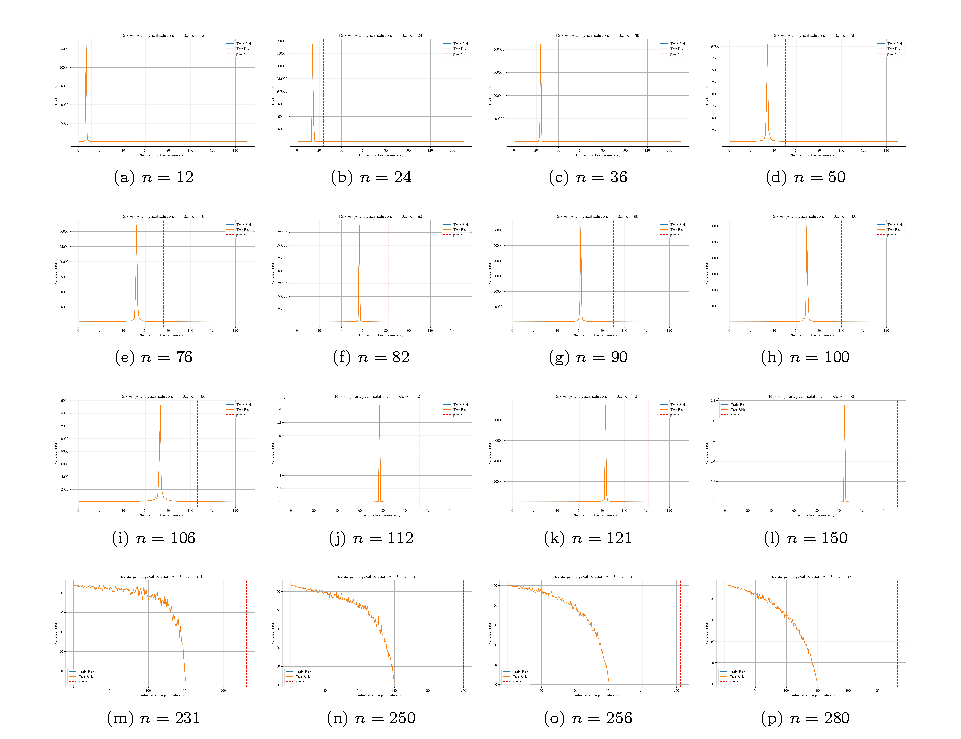
\includegraphics[width=0.8\textwidth]{pdf/theorem_4_verify.pdf}
    \caption{Risk curves for varying sample size $n$ (dimension $d=100$, noise $\sigma=0.5$). Double descent is determined in similar sequence, even though the interpolation theoretical $p=n$ is actually shifted over to the right from the actual interpolation observables, in parameterization. Afterward, correlation fails, and the theoretical $p$ is ineffective, similar to previous theorem-based test run. Sample set size range is $n\in\{12,24,36,50,76,82,90,100,106,112,121,150,231,250,256,280\}$. One additional remark is that the error landscape is relatively thin in either side, making it abnormal in comparison to actual bias-variance curvature.}
    \label{fig:theorem_double_descent_fig4}
\end{figure}

\subsubsection{Remark}

At least from this experiment, overall, results gathered using Theorem~\ref{thm:double_descent_lr} and variations of it suggests inconsistent results. The supposed interpolation threshold has different interpretation and indication in different scenario, including both parameter-wise error and prediction-only error measure. Furthermore, verification also shows inconsistency with the interpolation threshold, albeit given the fact that the margin of error from the highest peak to the interpolation point is consistent up to certain $n$. Breakdown of the result from theorem, as well as double descent behaviour starts with high $n$ counts, as well as interesting outlook of bias-variance reappearance for $p\sim 5000$, far more than what is tested in normal testing cases. Such result suggests further experiments to validate the observations, as well as statistical analysis of the entire system. 

Specifically, the interpretation of the result is not perfect. Under such setting, then for the concept of the same class, so $d=150$, any concept of $p>d$ would result in the metric taking zero value of the `truncated region' where $d$ is literally flat on the $d+1$ onward space. Hence, the error being added on top of such error measure is the component distance of $p$ to the flat sub $p-d$ space itself - which explains the curve going upward, as more and more risks are configured. Nevertheless, the amount of data provided, at least in terms of this model, does indeed have non-trivial effect on the model itself, and the least square solution of best fit which gives the potential minimal, hence the empirical best. Considering the results, we can see regions where the theorem `breaks' of its bias-variance pattern. Further experiment to verify such claim and reconfiguration is needed. Worryingly, in this particular case, there exists no saddle point that was theorized by bias-variance tradeoff, which must then be explained accordingly. Furthermore, we also notice the troublesome fact that this particular pattern works on \textit{same operational space} models, that is, linear models approximating linear models. This setting is fairly limited, and would not generalize well. However, we also do not know what kind of measure to take in such case. Conflicting notions and reports aid into the confusion of such topic more than can be normally observed, and the anomalous behaviours in some researches (for example, in \cite{shi2024homophilymodulatesdoubledescent}, we received that in GNN, there exists no trace of double descent) makes it even harder. As such, both the status of bias-variance being false, albeit in a given range only, and double descent in masking certain behaviours of the modelling process, have taken a mysterious stance in the modern machine learning community.

While discovering the double descent phenomena, it also exposes theoretical concepts that are not organized or formalized, portions of the theory and empirical observations that are within conflict of each others, issues with definitions, theorems, and interpretation of them. Those problems would then ultimately hinder further research in such direction, as well as broader theoretical requirement of the theory of machine learning, and specifically to a larger and more complex system of deep learning. 

\section*{Appendix B. A way of defining representation scheme}

Nevertheless, how to measure this complexity? We are not so sure how, but we can empirical formulate one, but will be fairly difficult to translate this to, since the representation complexity is often encoded in the sense of binary sequence or very old consideration of learning process of \cite{10.5555/200548}. Assuming abstraction of the bits/byte practical mathematical representation of numerical encoding (of which we will have to talk about later), we present the definition for the \textit{structural representation scheme} (basically a more applicable definition)

\begin{definition}[Representation scheme, structural definition]
    For a system and its object, an object's \textbf{representation scheme} $\mathcal{R}$ is a function $\bm{\mathcal{R}}: (\Sigma\cup \mathcal{G})^{*}\to \mathcal{O}$, where $\Sigma$ is the operator alphabet, or relational structure, $\mathcal{G}$ are the components, and $\mathcal{O}$ is the object. $(\Sigma \cup \mathcal{O})^{*}$ is the coupling of \textbf{all} configuration of the components and the operators. 
\end{definition}

In case where scalar numbers are presented, for example, in the axis-aligned rectangle case, we will have: $\bm{\mathcal{R}}^{2}_{\square}:(\Sigma\cup \mathcal{G}\cup\mathbb{F})^{*}\to \mathsf{Rec}$ of all rectangle using this representation scheme, so 

\begin{equation}
    \bm{\mathcal{R}}_{\square} = \begin{cases}
        \Sigma = \{\leq, \land \}\\
        \mathcal{G} = \{l_{c}, p_{c}, a\}\\
        \mathbb{F} = \mathbb{R}
    \end{cases}
\end{equation}
For example, of the formula of all concepts $c$ being axis-aligned rectangle, we can have the representation scheme in general as: 
\begin{equation}
    \sigma = \{c\} = \bm{\mathcal{R}}^{2} = \{a(x_{a},y_{a}) \mid l_{c}^{(1)} \leq x_{a}\leq p_{c}^{(1)}\land l_{c}^{(2} \leq x_{y}\leq p_{c}^{(2)}\}
\end{equation}

Generally, this is called the \textit{numerical representation scheme}, in which it is supported by a field (we do not care much about the dimension of the field, as long as we can decompose it to discrete scalar taking values), that is, $\bm{\mathcal{R}}:(\Sigma \cup \mathcal{G}\cup \mathcal{F})\to \mathcal{O}$. Any representation specification $\sigma\in (\Sigma \cup \mathcal{G}\cup \mathcal{F})$ such that $\bcal{R}(\sigma) = c$ is a representation of $c$ on $\bcal{R}$, denoted $\sigma_{c}$, and the set of all such specification $R_{c}=\{\sigma_{c}\}$ is called the \textbf{representation space} of $c$ on $\bcal{R}$.

The set of all hypotheses $h$ that is specified by certain representation scheme $\bm{\mathcal{R}}_{h}$ is called the \textit{hypothesis class} $\mathcal{H}$, and $\bm{\mathcal{R}}_{h}$ is the \textit{hypothesis class representation}. Similarly, for a concept $c$ the set of all concepts that are represented by $\bm{\mathcal{R}}_{c}$ is called the \textit{concept class} $\mathcal{C}$ for the \textit{concept representation scheme} $\bm{\mathcal{R}}_{c}$.

The necessity of the description of a field is rather natural, especially since we are working on a numerical encoding. Generally speaking, the computer at large represents a very complex binary encoding of numerical logical operations, though via abstractions, most of them are 'cancelled out' of the fundamental details. We can almost make a \textit{representation space} just similar to how we define vector space, though, it is more or less not so effective as it can.
Using this, we can specify quite a few object classes in the same way. The first one though, we can specify the representation scheme of an input-output model. Now, for this type of definition, then the class of all \textbf{linear function representation} can be designed as 
\begin{equation}
    \bm{\mathcal{R}}_{L}^{n} = \left\{ \{x_{1},\dots,x_{n}\}, y \Bigg| \sum_{i=1}^{n}w_{i}x_{i} + b \land w_{i}, x_{i}, b \in \mathbb{R} \right\}
\end{equation}
From this, we can notice that there exists the notion of \textit{size} for the object class. In one way or another, we have abstracted of the class of all objects that can be specified in such a way that their representation falls into the range of such representation class. Then, we might want to consider the concept of a \textbf{representation complexity}, and the size of the class, denoted $size(\bm{\mathcal{R}})$. Do note that this is not defining the operational complexity, but simply the structure by itself. Which is why we might want to have the definition of an object in such system that we are considering.

Two representations $\bcal{R}_{A}$ and $\mathcal{R}_{B}$, they are said to be \textbf{equivalent} if one can convert objects from the first representation to the second one, and vice versa. Then two representations are said to be \textbf{equal} if their size is the same, assume that the representation scheme is equivalent. This prompts us to define the notion of the size of the representation, but before that, a general insight will be the follow through - you have to be able to reduce one to the others, and reverse. By then, essentially, \textit{you cannot compare apple to orange}, that is. Generally, the size of a representation class is defined the smallest representation of the object in the underlying representation. So, for your example of the linear function, then 
\begin{equation}
    size(c)=\min_{\sigma \in R_{c}}\{size(\sigma)\}
\end{equation}
which again, prompt us \textit{again}, to figure out the notion for $size(\sigma)$. Before then, and defining the object's descriptions, let's try to construct a few more 'mathematical construct' of the same type. A subtle remark can be made here, that the representation only, again, specify the parameters used to represent it, and the string accompanied by such representation. The overall total repetition, for example, of a certain variable, and operation succeedingly, is totally irrelevant. I just get the formula as a shorthand for that scheme up there, as it is. Which again, means that to specify it, you need both the components and how it is connected. Abstractly speaking, and generally speaking so. 

A fundamental flaw in such configuration is that for something like \textit{data-dependent representation}, one might say that its representational complexity is infinite, which is, at least under such definition, totally true. Nevertheless, we shall then see, that even under such situation, the main mass of which is `representative' of the concept would be finite, for there are noisy and dense data in which does not add more information than not to the concept class. 

We can examine for now the representation complexity up to operation-level as defined for polynomial space. 

\section*{Appendix C - Experimental setting}

Aside from the usual setting that was settled above preliminary sections, to contain this experiment, formalism in the experimenting concept is needed. For now, loose speaking and loosely contriving such, this experiment section and further experiment sections will follow the same design template, which is illustrated in Figure~\ref{fig:vapnik_scheme}. Unless explicitly said so, we conform to this template. 
\begin{figure}[htb]
  \centering
  \includegraphics[width=0.65\textwidth]{media/Diagramatic_Modelling_View.png}
  \caption{\textbf{Diagrammatic view for the ambiance space of the modelling scenario setting.} Under classical learning theory and consideration, such scheme is used for almost every aspect possible of the learner's action. $c\in\mathcal{C}, h\in \mathcal{H}$ described by the tuple $(\mathbf{w},\mathbf{s})$ of main (weight) parameters and special parameters (for example, bias), $\mathbf{I}$ as the input space. The 3-tuple $(\omega, k,m)$ is used for controlling the partitioning (for $k=2$ is the train-test split). Others include $P(\mathbf{I},c,h,\mathcal{D}_{c})$ as the theorized action sequence (where the concept is exhibited, or the where the observational space is formed) of supposed distribution $\mathcal{D}_{c}$, the supervisor $\text{Supervisor}(\nabla, \mathcal{A}, \{\Theta_{S}\})$ for the loss class $\nabla$, algorithm $\mathcal{A}$, and $\{\Theta_{S}\}$ of special parameters for the supervisor. Additionally, we also include the supposed randomized state generation, $\mathsf{RAND}_{i}(\theta_{i,j,k})$ of distinct controlling parameters and arbitrary pseudo-random shape.}
  \label{fig:vapnik_scheme}
\end{figure}

There are certainly a lot of things to talk about of, at least in conclusion of this particular structure. Explicitly, now we can illustrate partially, where each component of the complexity measure might measure, kind of learning criteria that bounds the learning setting, depends on the cofactors it receives. Firstly, let's see the PAC-learning criteria. The PAC-learning criteria specifically target the sample set, the supervising error, and the assumed structure of the concept class. Hence, we can see that there exists three main components, indicated in Figure~\ref{fig:vapnik_scheme_1}. A lot of details are missing, which is typical of the setting by itself. 

\section*{Appendix D - Statistical learning theory perspective}

By statistical learning theory, we observed that there are plenty tradeoffs, most notably the empirical-generalization tradeoff, though we would have to clarify what those terms are. Furthermore, there is also what can be seen to be the analogue bias-variance tradeoff in such sense, is the \textit{approximation-estimation tradeoff} of statistical learning theory, though it must be clarified that they are strictly not the same, as seen from \cite{brown2024biasvariance}. 

Informally, the empirical-generalization tradeoff can be said to be the balancing act between achieving the true generalization and the empirical best. To achieve the generalization best, the empirical best, for finite hypothesis $\mathcal{H}$ (\cite{10.5555/2371238}), 
\begin{equation}
  \lim_{n\to \infty} \left[\underset{\mathcal{S}_{n}\sim \mathcal{D}^{m}}{\mathbb{E}}(\hat{R}_{\mathcal{S}(h)})\right]  = R(h), \quad h\in \mathcal{H}
\end{equation} 
This follows by the law of large number, and the statistical-probabilistic interpretation of the learning setting. However, the tradeoff is not straightforward - it is rather considered between, for example, the time-complexity, sample-space size, and generalization best's reach of the model. That is, for large the dataset is, the easier it is to get a sample space that represents more and more of the actual concept. However, in exchange, time-complexity increases, and thereby, the ergonomic aspect must be also considered. It is also concerned of the fact that the empirical best is not the same as even the generalization best, thereby, one will want their hypothesis class to extend. By doing this, they extend the outreach of the hypothesis class, however make it unstable under random, iterative process typically used to train such model to target. 

This is also noticed and formulated in the concept of approximation-estimation tradeoff. We refer to \cite{10.5555/2371238,lafon_understanding_2024} for some analysis and mentions. 

Let $\mathcal{H}$ be a family of functions mapping $\mathcal{X}\to\{1,-1\}$. This is the particular case of \textbf{binary classification}, in which can be straightforwardly extended to different tasks and loss functions. The \textit{excess error} of a hypothesis $h\in\mathcal{H}$, is the difference between its error $R(h)$ and the Bayes error $R^{*}$. This can be decomposed to be the following: 

\begin{equation}
    R(h) - R^{*} = \Big( R(h) - \inf_{h\in \mathcal{H}} R(h) \Big) + \Big( \inf_{h\in \mathcal{H}} R(h) - R^{*} \Big)
\end{equation}

The first bracket contains the \textbf{estimation error}, and the second bracket contains what is called the \textbf{approximation error}. The estimation error depends on the hypothesis $h$ selected. It measures the error of $h$ with respect to the infimum of the error achieved by hypotheses in $\mathcal{H}$, or that of the best-in-class hypothesis $h^{*}$ when that infimum is reached. The approximation error measures how well the Bayes error can be approximated using $\mathcal{H}$. It is a property of the hypothesis set $\mathcal{H}$, a measure of its richness. 

\section*{Appendix E - Observing gradient descent decomposition}

While the interpretation of what the bias-variance tradeoff, the usual training-versus-test curve, and statistical learning consideration, another interesting aspect to consider (as well for double descent), is how bias-variance decomposition acts on gradient descent and its components. This claim is perhaps reinforced by the work of \cite{adlam2020understandingdoubledescentrequires} which indicates that different bias-variance decompositions effects differently on the total system mechanism. 

\begin{figure*}[htb]
    \centering
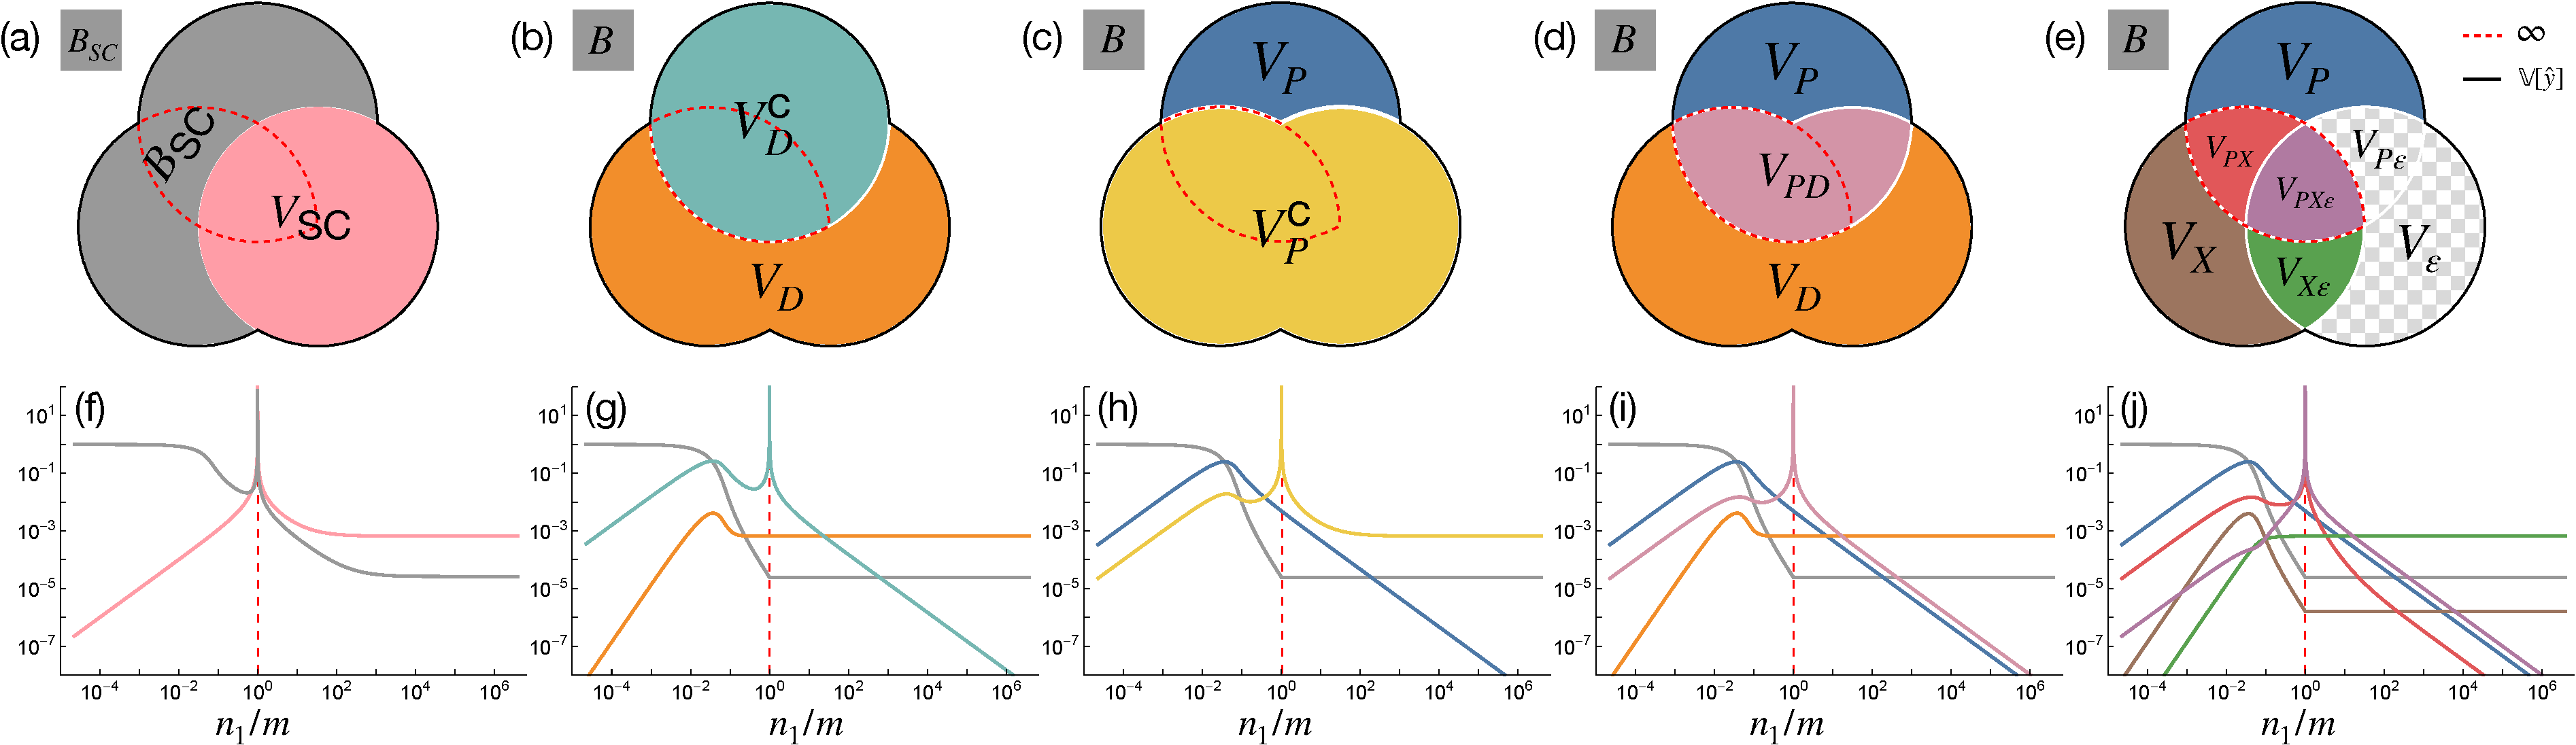
\includegraphics[width=\linewidth]{pdf/VennFig2.pdf}
\caption{(\textbf{a-e) The different bias-variance decompositions.} (f-j) Corresponding theoretical predictions for $\gamma =0$, $\phi=1/16$ and $\fs = \tanh$ with $\text{SNR} = 100$ as the model capacity varies across the interpolation threshold (dashed red). (a,f) The semi-classical decomposition of~\cite{hastie2019surprises,mei2019generalization} has a nonmonotonic and divergent bias term, conflicting with standard definitions of the bias. (b,g) The decomposition of~\cite{neal2018modern} utilizing the law of total variance interprets the diverging term $V_D^\textsc{c}$ as ``variance due to optimization''. (c,h) An alternative application of the law of total variance suggests the opposite, \emph{i.e.} the diverging term $V_P^\textsc{c}$ comes from ``variance due to sampling''. (d,i) A bivariate symmetric decomposition of the variance resolves this ambiguity and shows that the diverging term is actually $V_{PD}$, \emph{i.e.} ``the variance explained by the parameters and data together beyond what they explain individually.'' (e,j) A trivariate symmetric decomposition reveals that the divergence comes from two terms, $V_{PX}$ and $V_{PX\bfe}$ (outlined in dashed red), and shows that label noise exacerbates but does not cause double descent. Since $V_\e=V_{P\e}=0$, they are not shown in (j). Taken from \cite{adlam2020understandingdoubledescentrequires}}
\label{fig:venn_variance}
\end{figure*}

The main term of a gradient descent algorithm is the gradient of the loss function $\mathcal{L}(h(x),y)$. For the hypothesis $h$, the number of instances supplied denoted by $k$ has three main cases: $k=1$ for stochastic descent, $k\in (1,m)$ for batch gradient descent, and $k=m$ for standard gradient descent, for a given space of $m$ samples. The gradient in such case is calculated using the empirical risk on $m$ size, that is: 
\begin{equation}
    \mathcal{L}_{k}(h(x),y) = \hat{R}_{S[k]}(h) = \frac{1}{k} \sum^{k}_{i=1} \ell(h(x_{i}),y_{i})
\end{equation}
We use the classical bias-variance tradeoff at first. Since the gradient is a linear operator, we have: 
\begin{equation}
    \begin{split}
        \nabla_{k}(\mathcal{L}) &= \nabla_{k}\left(\pa{\E\hat{y}(\bfx) - \E y(\bfx)}^2 + \V\qa{\hat{y}(\bfx)} + \V\q{y(\bfx)}\right)\\
        & = \nabla_{k}\left( \E\left[\hat{y}(\bfx)\right] - \E\left[y(\bfx)\right] \right)^2 + \nabla_{k}\V\left[\hat{y}(\bfx)\right] + \nabla_{k}\V\left[y(\bfx)\right] \\
        & = \nabla_{k}\left( \E\left[\hat{y}(\bfx)\right] - \E\left[y(\bfx)\right] \right)^2 + \nabla_{k}\V\left[y(\bfx)\right]
    \end{split}
\end{equation}
This effectively decompose the gradient into three parts that influence the overall gradient calculation. Because $\nabla_{k}\V\left[y(\bfx)\right]$ calculates the gradient of irreducible error, which is supposed to be constant of the sample space, it is then equal $0$. Suppose a sample $\mathbf{x}_{k}$ of size $km$, of partition $k$. Hence, we have gradient descent based on $k$th run over the entire dataset, permuted. Then, the loss function calculates in the form 
\begin{equation}
  \nabla_{k,n}(\mathcal{L}) = \nabla_{k,n}\left[ \frac{1}{n}\sum_{i\leq n} \hat{y}(x_{kn+i})  - \frac{1}{n}\sum_{i\leq n} y(x_{kn+i}) \right]^{2} + \nabla_{k,n} \left[ \frac{1}{n}\sum_{i=1}^n y(x_i)^2 - \left( \frac{1}{n}\sum_{i=1}^n y(x_i) \right)^2 \right]
\end{equation}
The indices is now changed to $(k,n)$ for $m/k=n$ as the $i$th partitioned, ordered run, thereby $kn+i$ runs for the index. If we assume a simplified structure $\theta_{t}$ of parameters $y(x_{i})$ depends on, we can reduce it further.  
\begin{align}
\nabla_{k,n}(\mathcal{L})
&= 2\left(\frac{1}{n}\sum_{i\le n}\hat{y}(x_{kn+i}) - \frac{1}{n}\sum_{i\le n}y(x_{kn+i})\right)
   \left(\frac{1}{n}\sum_{i\le n}\nabla_k\hat{y}(x_{kn+i}) - \frac{1}{n}\sum_{i\le n}\nabla_k y(x_{kn+i})\right) \\
&+ \frac{2}{n}\sum_{i=1}^n y(x_i)\nabla_k y(x_i)
   - \frac{2}{n^2}\left(\sum_{i=1}^n y(x_i)\right)\left(\sum_{i=1}^n \nabla_k y(x_i)\right)\\
   & = = 2 \left(
   \left( \mathbb{E}_n[\hat{Y}] - \mathbb{E}_n[Y] \right)
   \left( \mathbb{E}_n[\hat{G}_k] - \mathbb{E}_n[G_k] \right)
   + \mathbb{E}_n[Y G_k] - \mathbb{E}_n[Y] \,\mathbb{E}_n[G_k]
\right)\\
&= 2 \left( 
   \left( \mathbb{E}_n[\hat{Y}] - \mathbb{E}_n[Y] \right)
   \left( \mathbb{E}_n[\nabla_k \hat{Y}] - \mathbb{E}_n[\nabla_k Y] \right)
   + \mathrm{Cov}_n\!\left(Y, \nabla_k Y\right)
\right) \\
& = 2 
   \left( \mathbb{E}_n[\hat{Y}] - \mathbb{E}_n[Y] \right)
   \left( \mathbb{E}_n[\nabla_k \hat{Y}] - \mathbb{E}_n[\nabla_k Y] \right) + 2\mathrm{Cov}_n\!\left(Y, \nabla_k Y\right)
\end{align}
for 
\begin{equation}
    \mathbb{E}_n[Z] = \frac{1}{n} \sum_{i=1}^n Z_i,
\qquad
\mathrm{Cov}_n(U,V) = \mathbb{E}_n[UV] - \mathbb{E}_n[U] \,\mathbb{E}_n[V].
\end{equation}
Here, we can see two terms multiplication, for the first one being the correlation between the expected error $\mathbb{E}_n[\hat{Y}] - \mathbb{E}_n[Y]$ and the gradient $\mathbb{E}_n[\nabla_k \hat{Y}] - \mathbb{E}_n[\nabla_k Y]$. This measures the correlation between the expected error, and the gradient measure. The second term is exactly the empirical covariance between the target $Y$ and the true gradient component. Since we are taking a fixed concept case, we can simply disregard the truth gradient hence $\mathbb{E}_n[\nabla_k Y]$, for which the term is reduced to $2\left( \mathbb{E}_n[\hat{Y}] - \mathbb{E}_n[Y] \right) \left( \mathbb{E}_n[\nabla_k \hat{Y}] \right)$. Under this same assumption applied to the covariance term, we obtain
\begin{equation}
    \nabla_{k,n}(\mathcal{L})
= \frac{2}{n}\sum_{i=1}^n \big(\hat Y_i - Y_i\big)\,\partial_k \hat Y_i = 2\left(
   \left( \mathbb{E}_n[\hat{Y}] - \mathbb{E}_n[Y] \right)
   \mathbb{E}_n[\nabla_k \hat{Y}]
\right)
\end{equation}
Looking into some particular algebraic representation, we can write this simply as
\begin{align}
    \nabla_{k,n}\mathcal{L}
    &= 2\,\mathbb{E}_n\!\left[(\hat Y - Y)\,\nabla_k \hat Y\right] \\
    &= 2\Bigg(
    \underset{\left[\mathbb{B}(\hat{Y},Y)\right]^{1/2}}{\underbrace{\bigl(\mathbb{E}_n[\hat Y] - \mathbb{E}_n[Y]\bigr)}}\,\mathbb{E}_n[\nabla_k \hat Y]
    + \underset{\mathrm{Cov}_n(\hat Y,\,\nabla_k \hat Y)}{\underbrace{\mathbb{E}_n[\hat Y\,\nabla_k \hat Y] - \mathbb{E}_n[\hat Y]\,\mathbb{E}_n[\nabla_k \hat Y]}}
     \\
    & \quad \quad \quad \quad \quad -\underset{\mathrm{Cov}_n(Y,\,\nabla_k \hat Y)}{\underbrace{\mathbb{E}_n[Y\,\nabla_k \hat Y] - \mathbb{E}_n[Y]\,\mathbb{E}_n[\nabla_k \hat Y]}}
    \Bigg)
\end{align}

The first term can be attributed to self-correct of bias-error gradient correlation, while the two covariance term suggests correlation between model randomness and its gradient, and the last one deal with the truth-gradient correlation. What those gradients mean will have to be tested in some preliminary models. Generally, we should not expect the result to be quite effective. Similar decomposition can be conducted for the other decomposition, as suggested, however, the gradient effect is particularly interesting, and will have to be resolved. 

\section*{Appendix F - Details of supervised learning structure}

In a typical machine learning setting, we obtain assume the following figure~\ref{fig:PhaseDiagram}. This includes the ground, input space (the setting of which the observations are observed), the concept $c\in\mathcal{C}$, the hypothesis $c\in \mathcal{H}$, and a supervisor $\nabla$ that `correct' the behaviours of the hypothesis to match with $c$. This is called a supervised learning setting, in which the learning part is governed by the supervisor and the observations from the concept.

\begin{figure}[!ht]
    \centering
    \captionsetup{font=small}
    \resizebox{0.7\textwidth}{!}{%
    \begin{circuitikz}
    \tikzstyle{every node}=[font=\normalsize]
    \draw  (6.25,20.5) rectangle  node {\normalsize $\mathbf{X}$} (7.5,15.5);
    \draw [->, >=Stealth, dashed] (7.5,19.25) -- (10,19.25)node[pos=0.5, fill=white]{$x\in\mathbf{X}$};
    \draw  (10,17.25) rectangle  node {\normalsize $h\in\mathcal{H}$} (13.75,16.25);
    \draw  (10,19.75) rectangle  node {\normalsize $c\in\mathcal{C}$} (13.75,18.75);
    \draw  (16.25,20.5) rectangle  node {\normalsize $\nabla(\cdot)$} (17.5,15.5);
    \draw [->, >=Stealth] (13.75,19.25) -- (16.25,19.25)node[pos=0.5, fill=white]{$c(X)$};
    \draw [->, >=Stealth] (13.75,16.75) -- (16.25,16.75)node[pos=0.5, fill=white]{$h(X)$};
    \draw [->, >=Stealth, dashed] (16.25,16.75) .. controls (14.75,15.25) and (12.25,15.25) .. (12,16.25)node[pos=0.5, fill=white]{$\mathsf{Update}$};
    \draw [->, >=Stealth, dashed] (7.5,16.75) -- (10,16.75)node[pos=0.5, fill=white]{$x$$\in$$\mathbf{X}$};
    %\draw [dashed] (5.5,21) rectangle  (9,15) node[below=2pt, pos=0.5] {\normalsize $I$};
    %\draw [dashed] (9.5,21) rectangle  (14.25,15) node[below=2pt, pos=0.5] {\normalsize $II$};
    %\draw [dashed] (14.75,21) rectangle  (18.5,15) node[below=2pt, pos=0.5] {\normalsize $III$};
    \draw [dashed] (5.5,21) rectangle (9,15);
    \node at ($(5.5,15)!0.5!(9,15) + (0,-7pt)$) {\normalsize $\mathrm{I}$};
    
    \draw [dashed] (9.5,21) rectangle (14.25,15);
    \node at ($(9.5,15)!0.5!(14.25,15) + (0,-7pt)$) {\normalsize $\mathrm{II}$};
    
    \draw [dashed] (14.75,21) rectangle (18.5,15);
    \node at ($(14.75,15)!0.5!(18.5,15) + (0,-7pt)$) {\normalsize $\mathrm{III}$};
    \end{circuitikz}
    }%
    \caption{An illustration of the (supervised) statistical process. Phase III contains two parts: First is the evaluation $\nabla(h,c)$ according to the data $\mathcal{D}$, and second is the $\mathsf{Update}$ process to re-align $c$ to the actual target.}
    \label{fig:PhaseDiagram}
\end{figure}
\subsection*{Phase 1.}
Begin with the construction and initialization of the feature space $\mathcal{X}^{\infty}$. By the assumption of a probabilistic process, $\mathcal{X}_{m}$ or simply $\mathcal{X}$ representing the dataset is assumed to be sampled, or appeared from the distribution $\mathcal{D}(p,\cdot)$ for $p$ an arbitrary probabilistic system. 

The \textit{ground space}, or in literature generally called \textbf{feature space}, is created. This results in the first component of the tuple $D$, being $\mathcal{X}\subseteq \mathbb{R}^{m\times k}$, where $\lvert \mathcal{X} \rvert=m$, but $size(x)=k$, for $x\in\mathcal{X}$. We assume there exists the random variable $x$ of a given distribution $\mathcal{D}$, such that the set $\mathcal{X}\sim \mathcal{D}$ of all observation is given by an underlying distribution. A well-known assumption in this case is that $x\in\mathcal{X}$ has no dependent components. That is, for example, there does not exist any function $\psi_{x}: \{ x_{i} \}\to \{ x_{j} \}$, for $i\neq j$. (Thought, this only helps in Bayesian priori analysis). Furthermore, by specifying that $\mathcal{X}$ belongs to a specific distribution, we argue of the assumption that $x\in\mathcal{X}$ is \textit{independently and identically distributed} (i.i.d.), that is, for a given random sampling interpretation $S\subset\mathcal{X}\sim \mathcal{D}$, all data is sampled with the events space governed by the distribution $\mathcal{D}$ for every instance, and the existence of $x_{i}$ to $x_{j}$ for $i\neq j$ is none. 

The \textbf{role} of the distribution configuration is important. If $\mathcal{D}$ is uniform, that is, $D\sim \mathcal{U}(a,b)$, then we can disregard the aspect of $\mathcal{X}$ with random variables. For $[a,b]$ to be $(-\infty,+\infty)$, the problem changed to a \textit{regression problem}. If $\mathcal{D}$ is some other distribution function, then the problem of \textit{representative data} and \textit{population size} becomes apparent, which requires statistical analysis to be taken into consideration. 
\subsection*{Phase 2.}
For the constructed feature space $\mathcal{X}$, let $EX(c,\mathcal{D})$ be a procedure (or \textit{oracle}) acting on $\mathcal{C}$ and $\mathcal{X}$ to output $\langle x,c(x)\rangle$. The hypothesis then contains a similar procedure $EX_{\mathcal{H}}(h,\mathcal{D})$, such that to output $\langle x,h(x)\rangle$. We call this the \textit{inference phase}. 
    
The feature space $\mathcal{X}$ is provided to $h$. We assume $c$ is processed of the same process, resulted in $\mathcal{Y}_{c}$. Then, $h(\mathcal{X})$ outputs the set of hypothesis' target $\mathcal{Y}_{h}$. Thereby, we are approximating the \textit{process} $c$ itself. We can approach this in two main ways\footnote{Note that, in some aspect, this is similar to the usage of mathematical simulation of certain dynamical system, or \textit{any} system that has certain patterns or relations observable.}: either \textit{deterministic} or \textit{probabilistic}\footnote{The model itself can be entirely deterministic, while the learning process is not. in fact, one of the very first assumption and axiomatic view of the learning problem is that learning occurs in a \textit{probabilistic setting}.}. We define such as followed. 
For the constructed feature space $\mathcal{X}$, let $EX(c,\mathcal{D})$ be a procedure (or \textit{orcale}) acting on $\mathcal{C}$ and $\mathcal{X}$ to output $\langle x,c(x)\rangle$. The hypothesis then contains a similar procedure $EX_{\mathcal{H}}(h,\mathcal{D})$, such that to output $\langle x,h(x)\rangle$. We call this the \textit{inference phase}. 
    

\begin{definition}[Deterministic - \textit{discriminative modelling}]
    A \textbf{deterministic model} $h_{d}$ assumes its internal space as followed. For any $h\in\mathcal{H}_{d}$ of deterministic model, $h$ is characterized by the mapping $h_{d}:\mathcal{X}\to \mathcal{Y}_{h}$, such that $h\in C^{n}$ of $n$-differential space. 
\end{definition}

Similarly, if the interpretation of the model is \textit{probabilistic}, we have the following definition of probabilistic-based model. 
\begin{definition}[Probabilistic - \textit{generative modelling}]
    A \textbf{probabilistic model} $h_{p}$ assumes its internal space as followed. For any $h\in\mathcal{H}_{p}$ of all probabilistic hypothesis, $h$ is characterized by the probability distribution $\Gamma(p_{X}(X))$, where $\Gamma$ is the discrete decision process outside the probabilistic interpretation. \footnote{The discrete decision process $\Gamma$ is very simple to argue. For example, given a Naive Bayes model with $p(C_{k}\mid D[i])$ of the dataset, the probability distribution is regarded as the argument $$Y^{*}=\underset{c_{k}\in C}{\mathrm{arg\:max}}\:P_{\theta}(c_{k}\mid x)=\underset{c_{k}\in C}{\mathrm{arg\:max}}P_{\theta}(x\mid c_{k})\cdot P(c_{k})$$}
\end{definition}
Notice that the process and the learning setting is probabilistic, however, the interpretation of the hypothesis $h$ can be either deterministic or probabilistic, or anything else. This puts the flexibility into the setting of the model, and permits us to consider various representation of the model structure. Furthermore, the hypothesis for the learning process is evaluated relative to the same probabilistic setting, in which the training takes place, and we allow hypotheses that are only approximation of the target concept \cite{10.5555/2930837,10.5555/200548}. 

The similarity between both of the two general types is that the model is characterized by their \textbf{parameters}, both \textbf{model-specific parameters} and \textbf{hyperparameters}. 
\subsection*{Phase 3.}
There exists an evaluator (or \textit{supervisor}) $\nabla (h,c)$ that evaluates specific \textit{loss framework} $\ell\{h(x),c(x)\}$ based on available information, and a \textit{update modifier} $U(\ell,\mathcal{A})$ of certain objective to algorithm $\mathcal{A}$. 
    
    In this step of the procedural setting, the \textit{supervisor} includes a loss function, $\ell$, which takes discrete arguments, and `binarily' evaluate the discrete result between $h$ and $c$. This loss function is supposed to have a global minimum, or at least a certain region of minimal approximation. We have the following definition. 

    \begin{definition}[Loss function]
        A loss function is a non-negative function $\ell :\mathcal{Y}\times\mathcal{Y}\to [0,+\infty)$. 
    \end{definition}
    
    In general, the following is supposed of the loss function: 
    \begin{conjecture}[Loss function convexity]
    For any supervisor $\nabla$ of a learner framework $\mathcal{L}(\mathcal{H},\mathcal{A})$, the loss function $\ell$ is assumed to be a $p$-converging function, or as a convex function. That is, for $\ell: \mathbb{R}^{n}\to \mathbb{R}$, then $\ell$ is convex on its domain, or is locally convex on $[a,b]\subset \mathbb{R}^{n}$, if, for $x,y\in\mathbb{R}^{n}$ of such interval, and for $\lambda \in [0,1]$, it satisfies \begin{equation}
        f(\lambda x + (1-\lambda)y) \leq \lambda f(x) + (1-\lambda) f(y)
    \end{equation}
    \end{conjecture}
Under a single structure, that is, for example, a class of mapping $\mathbb{R}^{n}\to\mathbb{R}$, there can exist many loss functions to be considered. Take for example the setting of regression analysis. Then, $\ell$ can be either the absolute error, $\lvert h(x)-c(x)\rvert$, or the $L^{2}$ norm, $\lvert\lvert h(x), c(x)\rvert\rvert_{2}$. Different loss function provides different path and landscape, though they still share somewhat similar interpolation patterns, or either some might be subjected to, under the consideration of a loss landscape, local minima than others. Furthermore, the form and representation of loss functions is not discrete - but rather based of its interpretation and the supposition of the underlying notion required for the loss function to operate in. For example, if the setting is \textit{generative}, the loss function would take the form of a \textit{divergence measure} between two probability distribution. Notice however, that the action potential provided by the model in their operation dissapears, or rather, is not considered, when using the loss function. 

Using such loss function, for the case of no noises or interference uncertainty, if the goal is to minimize the empirical risk on such dataset, then we call this the method of \textit{empirical risk minimization}, or ERM. This is born out of the consideration that in practice, the oracle $EX(c,\mathcal{D})$, and the actual generalization error $R(h)$ is not obtainable. 
\section*{Appendix F - Geman's derivation in \cite{6797087}}

\begin{proof}
    We present the original derivation of bias-variance tradeoff and its analysis from \cite{6797087}. Geman's paper is, by his own word, concerned of \textit{parametric models}, i.e. hypothesis class without strong assumption of parameters defined, though the definition of bias-variance tradeoff afterward and its justification is made in the sense of parametric model. We partially clarify\footnote{Generally, there is no definite definition on what would be considered non-parametric. Though, an example might be drawn from the (vanilla) neural network and Gaussian Process Regression (GPR)} this with the following definition as customary. 

    \begin{definition}[Parameterization]
        A \textbf{parametric model} is one that can be parameterized by a finite number of parameters. In general, for a hypothesis class $\mathcal{H}$of all parametric hypothesis is then expressed as:
        \begin{equation}
            \mathcal{H} = \{f(x;\theta): \theta \in \Theta \subset \mathbb{R}^{d}\}
        \end{equation} where $\Theta$ is called the \textit{parameter space}. A \textbf{nonparametric model} is one which cannot be parameterized by a fix number of parameters.   
    \end{definition}
    Suppose of a training dataset $\mathcal{D}$ of $N$ 2-tuples $(\mathbf{x}_{i},y_{i})$, that is: \begin{equation}
        \mathcal{D} = \{(\mathbf{x}_{1},y_{1}),\dots,(\mathbf{x}_{N},y_{N})\} \quad \lvert \mathcal{D} \rvert = N, \mathbf{x}\in \mathbb{R}^{d}, y \in \mathbb{R}
    \end{equation}
    The regression problem is to construct a function $f(\mathbf{x})\to y$ based on $\mathcal{D}$, which is denoted $f(\mathbf{x};\mathcal{D})$ to show this dependency. Then, 
    \begin{equation}
        \begin{split}
            \mathbb{E}\left[ (y-f(\mathbf{x};\mathcal{D}))^{2}\mid \mathbf{x},\mathcal{D}\right] & = \mathbb{E}\Big[\big( (y-\mathbb{E}[y\mid \mathbf{x}]+ (\mathbb{E}[y\mid \mathbf{x}]-f(\mathbf{x};\mathcal{D}))) \big)^{2}\mid \mathbf{x},\mathcal{D}\Big]\\
            & = \begin{multlined}
                \mathbb{E} \Big[ (y- \mathbb{E}[y\mid \mathbf{x}])^{2}\mid \mathbf{x},\mathcal{D} \Big] + \Big(\mathbb{E}[y\mid \mathbf{x}-f(\mathbf{x};\mathcal{D})]\Big)^{2} \\ + 2\mathbb{E} \big[(y-\mathbb{E}[y\mid \mathbf{x}])\mid \mathbf{x},\mathcal{D}\big]\cdot \big(\mathbb{E}[y\mid \mathbf{x}]-f(\mathbf{x;\mathcal{D}})\big)^{2} 
            \end{multlined} \\
            & = \mathbb{E} \Big[(y-\mathbb{E}[y\mid \mathbf{x}])\mid \mathbf{x},\mathcal{D}\Big] + \big(\mathbb{E}[y\mid \mathbf{x}]-f(\mathbf{x};\mathcal{D})\big)^{2}\\
            & \geq \mathbb{E} \big[(y-\mathbb{E}[y\mid \mathbf{x}])^{2}\mid \mathbf{x},\mathcal{D}\big]
        \end{split}
    \end{equation}
    Hence, we decompose it to: 
    \begin{equation}
        \mathbb{E} \left[((y-f(\mathbf{x};\mathcal{D})))^{2}\mid \mathbf{x}, \mathcal{D}\right] = \mathbb{E}\left[(y-\mathbb{E}[y\mid \mathbf{x}])^{2}\mid \mathbf{x},\mathcal{D}\right] + (f(\mathbf{x};\mathcal{D})-\mathbb{E}[y\mid \mathbf{x}])^{2}
    \end{equation}
    Where $\mathbb{E}\left[(y-\mathbb{E}[y\mid \mathbf{x}])^{2}\mid \mathbf{x},\mathcal{D}\right]$ is regarded to be a relative constant of variance on $y$ given $\mathbf{x}$. Taking the expectation on $\mathcal{D}$, we gain: 
    \begin{equation}
        \begin{split}
            \mathbb{E}_{\mathcal{D}} \Big\{ \mathbb{E} \left[((y-f(\mathbf{x};\mathcal{D})))^{2}\mid \mathbf{x}, \mathcal{D}\right]\Big\} & = \mathbb{E}_{\mathcal{D}} \Big\{\mathbb{E}\left[(y-\mathbb{E}[y\mid \mathbf{x}])^{2}\mid \mathbf{x},\mathcal{D}\right] + (f(\mathbf{x};\mathcal{D})-\mathbb{E}[y\mid \mathbf{x}])^{2}\Big\}\\
            & = \begin{multlined}
                \mathbb{E}_{\mathcal{D}} \Big\{ \mathbb{E}\left[(y-\mathbb{E}[y\mid \mathbf{x}])^{2}\mid \mathbf{x},\mathcal{D}\right]\Big\} \: + \\ \mathbb{E}_{\mathcal{D}} \Big\{ (f(\mathbf{x};\mathcal{D})-\mathbb{E}[y\mid \mathbf{x}])^{2}\Big\}
            \end{multlined}
        \end{split}
    \end{equation}
    The second term is of importance, and is further decomposed to: 
    \begin{equation}
        \begin{split}
            & \mathbb{E}_{\mathcal{D}} \Big\{ (f(\mathbf{x};\mathcal{D})-\mathbb{E}[y\mid \mathbf{x}])^{2}\Big\} \\ 
            & = \mathbb{E}_{\mathcal{D}} \Big\{ (f(\mathbf{x};\mathcal{D})- \mathbb{E}_{\mathcal{D}}[f(\mathbf{x};\mathcal{D})] + \mathbb{E}_{\mathcal{D}}[f(\mathbf{x};\mathcal{D})] -\mathbb{E}[y\mid \mathbf{x}])^{2}\Big\} \\
            & = \begin{multlined}
                \mathbb{E}_{\mathcal{D}} \Big[(f(\mathbf{x};\mathcal{D})-\mathbb{E}_{\mathcal{D}}[f(\mathbf{x};\mathcal{D})])^{2}\Big] + \mathbb{E}_{\mathcal{D}} \Big[ (\mathbb{E}_{\mathcal{D}} [f(\mathbf{x};\mathcal{D})] - \mathbb{E}[y\mid \mathbf{x}])^{2} \Big] + \\2\mathbb{E}_{\mathcal{D}}\Big[f(\mathbf{x};\mathcal{D})-\mathbb{E}_{\mathcal{D}}[f(\mathbf{x};\mathcal{D})]\Big]\cdot (\mathbb{E}_{\mathcal{D}}[f(\mathbf{x};\mathcal{D})]-\mathbb{E}[y\mid \mathbf{x}])
            \end{multlined} \\
            & = \underbrace{\left\{ \mathbb{E}_{\mathcal{D}}[f(x;\mathcal{D})] - \mathbb{E}[y\mid x] \right\}}_{\text{bias term}} + \underbrace{\mathbb{E}_{\mathcal{D}} \left\{(f(x;\mathcal{D})- \mathbb{E}_{\mathcal{D}}[f(x;\mathcal{D})])^{2}\right\}}_{\text{variance term}}
        \end{split}
    \end{equation}
    which yields the desired bias-variance tradeoff. 
\end{proof}


\end{document}
